\documentclass[12pt,a4paper]{report}

\usepackage{amsmath}
\usepackage{amsfonts}
%\usepackage{amssymb}
\usepackage{graphicx}
\usepackage{float}
\usepackage[autostyle]{csquotes}
\usepackage{acronym}
\usepackage{babel}
\usepackage{url}
\usepackage{algorithm}
\usepackage[noend]{algpseudocode}
\usepackage{tikz}
\usepackage{tabularx}
\usepackage{array}
%\usepackage{subfig}
\usepackage{titlesec}
\usepackage{caption}
\usepackage{subcaption}
\usepackage{mdframed}
\usepackage[legacy]{csvsimple}
\usepackage{siunitx}
\usepackage{url}

\usepackage[left=2cm,right=2cm,top=2.5cm,bottom=2.5cm]{geometry}

\usepackage[style=nature]{biblatex}
\addbibresource{sources.bib}

\newcolumntype{L}{>{\raggedright\arraybackslash}p}
\newcommand{\re}[1]{\textbf{\textcolor{orange}{#1}}}
\newcommand{\add}[1]{\textbf{\textcolor{blue}{#1}}}

\DeclareMathOperator*{\argmax}{argmax}

%\titleformat{\chapter}[display]
%{\normalfont\bfseries}{}{0pt}{\Large}


\title{
	A Sociable Virus? \\
	A Comparison and Investigation of Reproducibility of Methods for Analysing COVID-19 Transmission Chains Using Graph Networks
}


\author{Simon Westfechtel}

\begin{document}
	\emergencystretch 3em
	%\maketitle
	\begin{titlepage}
		\begin{center}
			\vspace*{1cm}
			
			\Huge
			\textbf{A Sociable Virus?}
			
			\vspace{0.5cm}
			\LARGE
			A Comparison and Investigation of Reproducibility of Methods for Analysing COVID-19 Transmission Chains Using Graph Networks
			
			\vspace{1cm}
			\large
			\textcolor{gray}{\textbf{Ein geselliges Virus?}}
			
			\vspace{0.5cm}
			\normalsize
			\textcolor{gray}{Ein Vergleich und eine Untersuchung der Reproduzierbarkeit von Methoden zur Analyse von COVID-19 Übertragungsketten mit Graphnetzwerken}
			
			\vfill
			
			\LARGE
			Master Thesis
			
			\large
			\textcolor{gray}{Masterarbeit}
			
			\vspace{0.4cm}
			
			\LARGE
			Computational Social Systems
			
			\vspace{0.8cm}
			
			\large
			Simon Westfechtel\\
			Matr.-Nr. 353822\\
			Aachen, \today
			\vfill
			
			\Large
			RWTH Aachen University\\
			Chair for Computational Social Sciences and Humanities\\
			
			\vfill
			\begin{flushleft}
				\normalsize
				Primary Supervisor / Erstprüfer: Priv.-Doz. Dr. Jürgen Lerner\\
				Secondary Supervisor / Zweitprüferin: Dr. Nazmiye Gizem Bacaksizlar Turbic\\
			\end{flushleft}
			
		\end{center}
	\end{titlepage}
	\begin{abstract}
		Scientific work on epidemics and pandemics mostly focuses on virology and potential treatments, while the societal aspect is often overlooked. The results are incoherent and often unfounded containment methods. The field of Computational Social Science offers a wide array of tools to analyse pandemic situations on a societal level. This work seeks to investigate and compare the usage of Social Network Analysis (SNA), Relational Event Models (REM) and Relational Hyperevent Models (RHEM) for this task. These methods are used to analyse six case contact networks from Europe and China. Results are compared to original reports where applicable to investigate reproducibility, and further compared horizontally (i.e. inter-regional) and vertically (i.e. inter-methodological). Results show a significant impact of age and sex on contact nomination likelihood, and a tendency for named contacts to become infected at later stages and interact with other contacts. Furthermore, Social Network Analysis and Relational (Hyper-)event Models should be used for different tasks. While no definitive answer can be given as to whether REM or RHEM are the preferable choice, findings justify the usage of RHEM over REM.  
	\end{abstract}
	\tableofcontents
	\chapter{1\quad Introduction}
\label{ch:Introduction}

When rumours of a novel respiratory virus, which would later be dubbed coronavirus disease 2019, or short COVID-19, first emerged from the People's Republic of China in late 2019, there was a lot of uncertainty regarding its danger potential. Authorities were hesitant to acknowledge the threat of a possible epidemic, and people were discouraged from stocking up on equipment such as protective face masks. When the virus spread to other countries across the globe and its impact could no longer be ignored, governments reversed course and imposed various restrictions on their respective populations, even going as far as sending a whole country into lockdown, in order to halt, or at least slow the spread of the virus. However, the sheer number of cases soon threatened to overwhelm healthcare systems worldwide.

In order to prevent this worst-case scenario, it became paramount to identify sources of infection and interrupt transmission chains. The efficient tracing of infected individuals' social contacts plays an integral part in preventing the spreading of a disease, and had been a well-established procedure well before the emergence of COVID-19, where for instance a verified case of tuberculosis requires a notification of the health departments \cite{enwiki_1097839709}. This is done to isolate persons who might have been infected by or have themselves been the source of infection of the individual, and therefore interrupt the transmission chain early, comparable to removing a domino piece to stop the fall of subsequent ones.

Most attention regarding science during the pandemic has focused on the medical field, especially the research of effective vaccines and treatments against the virus, but also virological factors (e.g. which individual features would predispose someone to infection and/or a severe course of illness, how the virus is transmitted from person to person, etc.). Now that the pandemic has mostly passed, a retrospective view suggests that there were no comprehensive insights into infection dynamics on a societal level, as evidenced by the at times incoherent measures taken in order to combat the spread of the virus.

It is therefore necessary to establish a set of methods to effectively and efficiently analyse the social aspects of viral transmission and spread in order to be better prepared for a similar situation in the future. In the recent months, more work tackling this topic has emerged, and the field of computational social sciences offers a wide array of tools to address this problem.

Computational Social Science (CSS) is an interdisciplinary field that uses advanced computa-tional methods to investigate social phenomena and human behavior. It combines elements of social sciences, such as sociology, economics, and psychology, with data science, computer science, and statistics. The aim is to glean insights into the complex dynamics of human societies through analysis of big data, modeling, and simulations, typically drawing from data sources like social media, web pages, or even administrative records.

The essence of CSS is the quantification and analysis of social phenomena, facilitating a deeper understanding of individual and group behaviors, social structures, and societal trends. By leveraging computational tools such as machine learning, network analysis, natural language processing, and agent-based modeling, CSS allows researchers to explore questions that were previously inaccessible due to the sheer complexity of the social systems involved. This often involves handling large and complex datasets, managing issues of privacy and ethics, and interpreting results in a meaningful social context.

\section{Contact Tracing}
\label{sec:contact_tracing}

Many contact tracing initiatives were established during the course of the pandemic in most developed countries, e.g. automatic tracing via mobile apps; although they differ in the level of detail that was (or still is) being recorded, data collected at least included the source of infection, i.e. a symptomatic or, once tests had become widely available, positively tested patient, and said patient's social contacts, i.e. the people who had come into contact with them, and who thus could have been infected themselves and possibly spread the virus further. More rigorous systems also recorded covariates such as age, job or co-morbidities, which may play a role in transmission. 

A dataset consisting of records of the form (source, contact) can be modelled as a social network, a concept derived from graph theory, where individuals constitute a set of vertices, and contacts between individuals are represented by edges between the respective vertices; for an illustration, refer to figure \ref{fig:example_case_network}. These networks can be efficiently analysed using methods stemming from the field of computer science; thus, it becomes possible to identify dynamics in the spread of the virus on a social level, which are traditionally overlooked in virology. Common network effects include betweenness centrality, a measure for how instrumental a person is in facilitating the viral spread, or community detection and shortest paths lengths to determine whether infections emerge in clusters. Additionally, if further covariates like age, pre-existing illness or profession were also collected during the contact tracing procedure, methods from the field of data science can reliably discover patterns in the data and thus identify covariates that influence transmission, e.g. whether younger people are more likely to get infected and/or infect others compared to other age groups.

\begin{figure}
	\begin{mdframed}
		\centering
		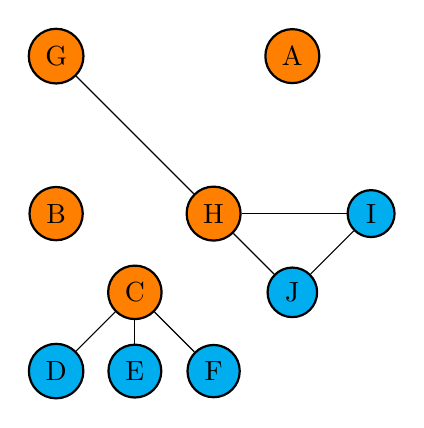
\begin{tikzpicture}
		\begin{scope}[every node/.style={circle,thick,draw,fill=orange}]
			\node (A) at (2,2) {A};
			\node (B) at (-1,0) {B};
			\node (G) at (-1,2) {G};
			\node (C) at (0,-1) {C};
			\node (H) at (1,0) {H};
		\end{scope}
		
		\begin{scope}[every node/.style={circle,thick,draw,fill=cyan}]
			\node (D) at (-1,-2) {D};
			\node (E) at (0,-2) {E};
			\node (F) at (1,-2) {F};
			\node (I) at (3,0) {I};
			\node (J) at (2,-1) {J};
		\end{scope}
		
		\begin{scope}
			\path (C) edge node {} (D);
			\path (C) edge node {} (E);
			\path (C) edge node {} (F);
			\path (G) edge node {} (H);
			\path (H) edge node {} (I);
			\path (H) edge node {} (J);
			\path (I) edge node {} (J);
		\end{scope}
	\end{tikzpicture}
	\caption{Exemplary case contact network. Confirmed cases are coloured orange, and reported contacts are coloured cyan. This network contains four connected components: $\{\{A\},\{B\},\{C,D,E,F\},\{G,H,I,J\}\}$}
	\label{fig:example_case_network}
	\end{mdframed}
\end{figure}

\section{Relational Event Models}
\label{sec:intro_rem}

These static networks, however, can only give a partial representation of reality, since temporal information is omitted; thus, it is assumed that all infections and contact nominations happen simultaneously, whereas in reality, events occur sequentially. Therefore, infected patient $A$ might name person $B$ as a contact at time $t_1$, and $B$ might himself be recorded as a patient at a later time $t_2$, nominate persons $C,D$ as contacts, and so on. Obviously, this temporal aspect leads to a range of additional possible effects. Do dyads (pairs of source, contact) appear repeatedly (repetition), is a person $B$ who gets nominated as a contact by $A$ at time $t_n$ more likely to become a patient, and nominate $A$ in return at a later time $t_{n+m}$ (reciprocation), or is there a tendency for cyclic closure, where $A$ nominates $B$, $B$ then nominates $C$, and $C$ nominates $A$?

A common method for modelling time-stamped relational data of the form (time, source, target) are Relational Event Models, short REM, which were first proposed by \cite{butts20084}. They will be discussed further in chapter \ref{ch:methods}.

\section{Relational Hyperevent Models}
\label{sec:intro_rhem}

An obvious shortcoming of relational event models is their dyadic nature, i.e. their inherent assumption that all interactions only involve two people at a time. Of course, this is not an accurate representation of reality. Think, for example, of John sending an email addressed at multiple of his colleagues, or in the context of COVID, Jane testing positive after attending a party and naming all the other guests as contacts. Some workarounds have been proposed to tackle this problem, like treating all interactions separately, or grouping all receiver nodes (email recipients and party attendees in our examples, respectively) into a single node. Refer to figure \ref{fig:polyadic_interactions} for an illustration. The problem with the former method is the fact that is treats the interactions as independent, while the latter may be unfeasible or even intractable for large datasets.

\begin{figure}
	\begin{mdframed}
		\centering
		\begin{subfigure}[t]{0.45\linewidth}
			\vskip 0pt
			\centering
			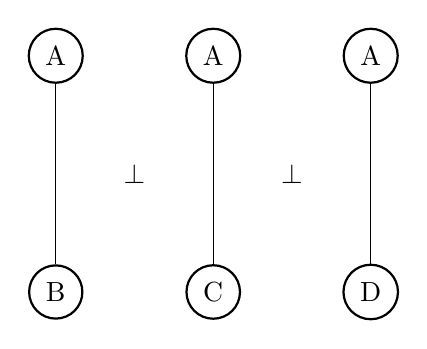
\begin{tikzpicture}
				\begin{scope}[every node/.style={circle,thick,draw}]
					\node (A1) at (0,0) {A};
					\node (A2) at (2,0) {A};
					\node (A3) at (4,0) {A};
					\node (B) at (0,-3) {B};
					\node (C) at (2,-3) {C};
					\node (D) at (4,-3) {D};
				\end{scope}
				
				\begin{scope}
					\node[draw=none] (A1A2) at (1,0) {};
					\node[draw=none] (BC) at (1,-3) {};
					\node[draw=none] (A2A3) at (3,0) {};
					\node[draw=none] (CD) at (3,-3) {};
				\end{scope}
				
				\begin{scope}
					\path (A1) edge node {} (B);
					\path (A2) edge node {} (C);
					\path (A3) edge node {} (D);
					\path (A1A2) edge[draw=none] node {$\perp$} (BC);
					\path (A2A3) edge[draw=none] node {$\perp$} (CD);
				\end{scope}
			\end{tikzpicture}
			\caption{Method 1: Model one edge for each node of the receiver set. Edges are assumed to be independent.}
		\end{subfigure}
		\hfill
		\begin{subfigure}[t]{0.45\linewidth}
			\vskip 0pt
			\centering
			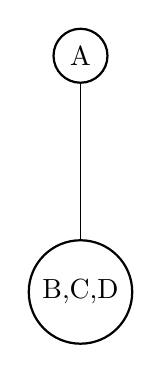
\begin{tikzpicture}
				\begin{scope}[every node/.style={circle,thick,draw}]
					\node (A) at (0,0) {A};
					\node (B) at (0,-3) {B,C,D};
				\end{scope}
				
				\begin{scope}
					\path (A) edge node {} (B);
				\end{scope}
			\end{tikzpicture}
			\caption{Method 2: Model receiver set as a single node}
		\end{subfigure}
	\caption{Two ways to approximate polydiadic interactions. In this example, $A$ has an interaction with $B, C,$ and $D$ at the same time (e.g. They meet for a drink at the pub and $A$ subsequently falls ill with Coronavirus).}
	\label{fig:polyadic_interactions}
	\end{mdframed}
\end{figure}

To address these issues, an extension to REM, named Relational Hyperevent Models, short RHEM, has been proposed by \cite{lerner2019rem}. These models use hyperedges instead of the regular, dyadic edges known from graph theory; each hyperedge consists of a sender (e.g. a positively tested patient) and a set of receivers (e.g. attendees of a birthday party). These models can be used to discover effects in a fashion similar to REM, but with additional effects specific to polyadic interactions like partial repetition, where the receiver set is only partially the same in a repeated interaction (e.g. John plays tennis with Jane and Max, gets ill and nominates Max and Jane at time $t_n$, and again gets sick after grabbing coffee with Jane and Peter at time $t_{n+m}$ and thereafter nominates them), or unordered repetition, where an interaction is repeated involving the same actors, but the direction is not the same (e.g. reaching back to the previous example, John, Jane and Max again meet for tennis, whereafter Jane tests positive and nominates John and Max as contacts at time $t_{n+m}$). These RHEM will likewise be discussed in chapter \ref{ch:methods} in more detail.

\section{Goal}
\label{sec:intro_goal}

This work's primary aim is to review three different methods that have been proposed for analysing COVID-19 case contact networks, namely Social Network Analysis (SNA), Relational Event Models (REM) and Relational Hyperevent Models (RHEM). This review process will consist of an investigation of reproducibility of previously reported results through the usage of equivalent methodology, and a comparison of results between these three methods. To this end, SNA, REM and RHEM will be used to analyse five distinct case contact networks. Results of these analyses are then compared horizontally, i.e. between datasets, and vertically, i.e. between methods. Chapter two will present and briefly discuss the research and data upon which this work relies and builds. Chapter three will recapitulate the theoretical fundamentals of SNA, REM and RHEM and outline how these methods are applied to the data. Analysis results will be presented and discussed in chapter 4. Finally, chapter 5 will give an outlook on possible future extensions of this work.
	\chapter{2\quad Previous Work and Data Exploration}
\label{ch:previous_work_data}

This work seeks to compare methods proposed and corresponding results presented by Yang et al. \cite{shaanxi_publication,hainan_publication} and Hâncean et al. \cite{hancean2022occupations}. As alluded to in chapter \ref{ch:Introduction}, static network modelling, relational event modelling and relational hyperevent modelling will be compared against each other. These three methods will be applied to five different datasets. One is from Bucharest, Romania, which has already been analysed using relational hyperevent models by Hâncean et al. \cite{hancean2022occupations}; three are from Yunnan, Hainan and Shanxi, China, which have all been analysed using static network models by Yang et al. \cite{hainan_publication,shaanxi_publication}; the final dataset comprises records from all of China, and has, to the knowledge of the author, not been analysed at the time of writing this.

All the Chinese datasets are structures in the same basic manner, where records name the person who is being registered as a positively tested case, henceforth also referred to as referee; the person who is being nominated as a contact (if any), henceforth also referred to as referral; as well as covariates for referee and referral. Thus, one row equals one case contact nomination. Refer to table \ref{tab:china_data_structure} for an example. For these datasets, referees and referrals have all been tested positive for the virus.

The Romanian dataset, in contrast, consists of two tables, where one table contains all contact nominations akin to the Chinese ones, and one table contains information on positively tested patients. The patient information table contains all referees, but not all referrals, meaning that not all registered individuals were tested positive. 
To express this formally, let $A$ be the set of referees, $B$ be the set of referrals, and $P$ be the set of positively tested patients. For the Yunnan, Hainan, Shanxi and China dataset, it is $P = A \cup B$; for the Bucharest dataset, it is $A \subset P$, $B \not\subset P$, $P = A \cup X$, where $X = B_1 \cup B_2; B_1 \subset P, B_2 \not\subset P$.

\begin{table}
	\begin{tabularx}{\linewidth}{XXXXX}
		\hline
		\textbf{Timestamp} & \textbf{Referee} & \textbf{Referral} & \textbf{Referee covars [...]} & \textbf{Referral covars [...]} \\
		\hline
		2020-06-01 & p10 & p14 & ... & ... \\
		2020-06-01 & p10 & p17 & ... & ... \\
		2020-06-03 & p12 & - & ... & ... \\
		$\cdots$ & & & & \\
	\end{tabularx}
	\caption{General structure of the Chinese datasets. One row is equal to one contact nomination. Rows where the referral is empty mean there was no person nominated as contact by the referee. In this example, patient p10 nominated persons p14 and p17 as contacts, who themselves have also been tested positive. Patient p12, meanwhile, has not named anyone as a social contact.}
	\label{tab:china_data_structure}
\end{table}

\section{Yunnan Dataset}
\label{sec:yunnan_data}

\paragraph{Dataset overview} This dataset contains COVID case information from the province of Yunnan in southern China \cite{hainan_data}. There are 171 entries, with dates ranging from 2020-01-17 to 2020-02-16, i.e. this dataset is from the very early stages of the pandemic. The patient covariates deemed to be relevant are age, gender, and whether they are relatives of other confirmed cases listed in the dataset. All covariates are also listed in table \ref{tab:yunnan_covariates}.

Of the 171 individuals who have been confirmed positive, 114 cases have named no contacts at all, 25 have named one contact, eleven have named two contacts, and 21 have named three contacts or more. 58 and 62 cases are female and male, respectively; this information has not been recorded for the remaining 51 patients. This suggests neither sex is more susceptible to the virus. The average age of patients is $41\pm18$, with a 25 percentile of 26 and a 75 percentile of 54, meaning patients are mostly younger or middle-aged. From the 60 cases where this information is available, 31 are family members of other patients present in the dataset. 

\begin{table}
	\begin{tabularx}{\linewidth}{XXX}
		\hline
		\textbf{Covariate} & \textbf{Description} & \textbf{Mean / Ratio / Range}\\
		\hline
		Date & Date when the case was confirmed/reported & 20/01/17 - 20/02/16\\
		Gender & Male/Female & $51.6\%$ \\
		Age & In years & $41\pm18$ \\
		Relatives & Whether the patient is a relative of previously recorded cases & $51.6\%$ \\
		\hline
	\end{tabularx}
	\caption{Relevant covariates for the Yunnan dataset}
	\label{tab:yunnan_covariates}
\end{table}

\paragraph{Network analysis}
As previously mentioned, this dataset was analysed by Yang et al. using network modelling \cite{hainan_publication}. In their work, they determined the effect of the aforementioned patient covariates like age and gender, as well as the following network effects:
\begin{itemize}
	\item degree centrality: a node-specific centrality measure, which is equal to the number of edges connected to a node $i$. Higher-degree nodes are therefore deemed more central, i.e. important, in the network \cite{golbeck}. In the context of case contact networks, these are the patients who nominate more contacts than average.
	\item betweenness centrality: a node-specific centrality measure, which for three nodes $i,j,k$ measures the ratio of the number of shortest paths from $j$ to $k$ that go through $i$ to the total number of shortest paths from $j$ to $k$. Nodes with a high betweenness centrality are nodes that facilitate the flow of information in the network, and are therefore deemed more central, i.e. important \cite{golbeck}. In the context of case context networks, these are the patients who are likely to have transmitted the virus from one cluster of patients to another.
	\item pagerank centrality: a node-specific centrality measure based on eigenvector centrality. It is computed by performing random walks on the network and measuring the likelihood to arrive at a node $p_i$ for all nodes. Nodes with a high pagerank centrality are frequently pointed at, and are therefore deemed more central, i.e. important \cite{gleich_pagerank}. In the context of case contact networks, these are patients who have been nominated as contacts more often than average.
	\item component size: connected components are sets of nodes in a network which are strongly connected, but have no outside connected, i.e. form a coherent and isolated community. In the context of case contact networks, these represent infection clusters, and the investigation of the size of these clusters can yield insights into how the virus tends to spread.
\end{itemize} They report an average degree centrality of $1.3\pm3.2$, an average betweenness centrality of $0\pm0$, and an average pagerank centrality of $0.0058\pm0.0055$. Furthermore, three of 18 connected components comprise of more than three nodes \cite{hainan_publication}. 

According to Yang et al., the zero value for betweenness centrality indicates that transmission of the virus from patient to patient happened near-simultaneously and in clusters, rather than in long transmission chains; A maximum pagerank score of 0.0221 compared to the mean value of $0.0058\pm0.0055$ means that ties are distributed unequally among patients, with a small number of patients being associated with most contact nominations. Furthermore, they write that the large fraction of nodes without ties is due to those patients hailing from another state, which made tracing of their contacts difficult; however, it isn't exactly stated why contact tracing was not possible for this group. The development of the case contact network over time was also analysed, albeit on a coarse level, where states of the network at three distinct points in time (start, middle and end point of the time period) were compared. Findings suggest that early cases were mostly imported from other provinces, since those mostly had no associated contacts, while local infection clusters only emerged in the later stages \cite{hainan_publication}. 

\section{Hainan Dataset}
\label{sec:hainan_data}

\paragraph{Dataset overview} This dataset contains COVID case information from the province of Hainan \cite{hainan_data}, which is the southernmost province of China. It was released in tandem with the Yunnan dataset, and therefore patient covariates are the same. There are 162 entries, with dates ranging from 2020-01-22 to 2020-02-14, i.e. this dataset is also from the early stages of the pandemic. Of the 162 confirmed cases, 71 have named no contacts, 27 have named one contact, 21 have named two contacts, and 43 have named three contacts or more. 

84 and 78 cases are female and male, respectively. An average age of $48\pm17$, a 25 percentile of 36 and a 75 percentile of 62 mean that the patients in this dataset are from an older age group compared to the Yunnan data. 75 out of 162 patients are family members of previously recorded cases.

\begin{table}
	\begin{tabularx}{\linewidth}{XXX}
		\hline
		\textbf{Covariate} & \textbf{Description} & \textbf{Mean / Ratio / Range}\\
		\hline
		Date & Date when the case was confirmed/reported & 20/01/22 - 20/02/14\\
		Gender & Male/Female & $48.2\%$ \\
		Age & In years & $48\pm17$ \\
		Relatives & Whether the patient is a relative of previously recorded cases & $46.3\%$ \\
		\hline
	\end{tabularx}
	\caption{Relevant covariates for the Hainan dataset}
	\label{tab:hainan_covariates}
\end{table}

\paragraph{Network analysis} This dataset was analysed by Yang et al. using the same methodology outlined in section \ref{sec:yunnan_data}. They report an average degree centrality of $1.51\pm1.79$, an average betweenness centrality of $0\pm0$, and an average pagerank centrality of $0.0062\pm0.0043$. Ten out of 27 connected components are comprised of more than three nodes \cite{hainan_publication}. 

Interpretation of these numbers is similar to the Yunnan network. The zero value for betweenness centrality again indicated transmission happening in clusters rather than chains, and a maximum pagerank score of 0.0189 compared to the mean $0.0062\pm0.0043$ suggests an uneven distribution of ties. However, the larger fraction of patients with contacts (57\% here vs. just 33\% in the Yunnan dataset), paired with the larger number of connected components (27 vs. 18) means that less cases were imported from other states and/or containment measures might not have been as effective (the authors state that imposed measures were largely the same for both Yunnan and Hainan provinces). Accordingly, the temporal development of the case contact network shows an earlier emergence of infection clusters \cite{hainan_publication}.

\section{Shaanxi Dataset}
\label{sec:shaanxi_data}

\paragraph{Dataset overview} This dataset contains COVID case information from the province of Shaanxi in northern China \cite{shaanxi_data}. There are 237 entries, with dates ranging from 2020-01-23 to 2020-02-16, so this dataset too is from the early stages. Relevant covariates are mostly equivalent to those of the previous two discussed sets, with the addition of the place of residence; covariates are listed in table \ref{tab:shanxi_covariates}. 

Of the 237 positively tested patients, 108 cases have named no contacts at all, 68 have named one contact, 36 have named two contacts, and 25 have named three contacts or more.  With 129 versus 108, there are slightly more men in this dataset compared to the near-equal distribution found in the previous two discussed datasets. The average age of patients is $46\pm17$, the 25 percentile is 35, and the 75 percentile is 59. Only 87 of the 237 patients are family members of previously recorded cases, suggesting that the majority of infections were transmitted from stranger to stranger rather than between family members; this is a contrast to the near-equal distribution found in the Yunnan and Hainan datasets (36.7\% vs. 51.6\% and 46.2\%, respectively). The three most common places of residence are \emph{Xian}, \emph{Ankang} and \emph{Hanzhong}.

\begin{table}
	\begin{tabularx}{\linewidth}{XXX}
		\hline
		\textbf{Covariate} & \textbf{Description} & \textbf{Mean / Ratio / Range}\\
		\hline
		Date & Date when the case was confirmed/reported & 20/01/23 - 20/02/16\\
		Gender & Male/Female & $54.4\%$ \\
		Age & In years & $46\pm17$ \\
		Relatives & Whether the patient is a relative of previously recorded cases & $36.7\%$\\
		Hukou & Place of residence & -\\
		\hline
	\end{tabularx}
	\caption{Relevant covariates for the Shanxi dataset}
	\label{tab:shanxi_covariates}
\end{table}

\paragraph{Network analysis} This dataset, too, was analysed by Yang. In addition to the previously discussed network statistics, closeness centrality was also included in the analysis. Closeness centrality a node-specific centrality measure, which is defined as the reciprocal of the sum of all shortest paths for a node $i$. Nodes with a high closeness centrality are nodes that are only a few edges away from other nodes, and are therefore deemed more central, i.e. important \cite{sabidussi1966centrality}. 

Reported were an average degree centrality of $.99\pm1.3$, an average closeness centrality of $0.45\pm0.44$, and average betweenness centrality of $0\pm0$, and an average pagerank centrality of $0.0042\pm0.0035$. 12 out of 40 connected components are comprised of more than three nodes. Interpretations are analogous to the other datasets; a tie to no-tie ratio of 54\% paired with the highest number of connected components yet suggest a tendency for cluster outbreaks similar to Hainan province, a fact which the author claims is corroborated by the average closeness centrality value \cite{shaanxi_publication}.

\section{Xi'an Dataset}
\label{sec:xian_data}

\paragraph{Dataset overview} This dataset contains COVID case information from the city of Xi'an, which is located in the Shaanxi province in northern China \cite{xian_data}. There are 2050 entries; unfortunately, despite being present in the corresponding research paper, neither dates nor patient covariates were included in the referenced dataset \cite{xian_publication,xian_data}. It's important to note that the article is merely a preprint version and its status is currently under major revision. Still, this dataset may provide interesting insights in the comparison of different regions. It is stated in the paper that dates range from 2021-12-09 to 2022-01-18, i.e. this network is the first to depict a mid-pandemic time period. 

Out of the 2050 positively tested patients, 965 cases have named no contacts at all, 871 have named one contact, 132 have named two contacts, and 82 have named three contacts or more. The average age of patients is $36\pm18$, and the male-to-female ratio is 55.5\% (1118 men vs. 932 women). There is no information regarding the 25 and 75 percentiles of patient age. 

\paragraph{Network analysis} Network statistics used by Yang are degree centrality, pagerank centrality, closeness centrality, betweenness centrality, component size and triadic census; the author explains that this means the count of possible triadic structures (ref. \ref{fig:triadic_structures}) present in the graph. They report those counts to be 545,154 for the 003 configuration, 1,550,928 for the 102 configuration, 1,752 for the 201 configuration, and 0 for the 300 configuration. Yang claims that triadic census can be used to analyse the spread pattern of the virus, but unfortunately does not elaborate further on this.

Values for degree centrality, pagerank centrality, closeness centrality and betweenness centrality are $0.7\pm1.4$, $0.0005\pm0.0006$, $0.4\pm0.4$, and $3.4\pm50.6$, respectively. The value for betweenness centrality is especially interesting since it was always zero up until now. This suggests that there were more transmission chains and/or different clusters connected by a single individual, as opposed to the isolated infection clusters that can be seen in the other datasets. The author provides no interpretation for the other statistics.

There are 1291 connected components, and 82 out of those consist of more than three nodes. Since this dataset is significantly larger than the ones discussed previously, these numbers are not directly comparable. This is addressed by computing the modularity score of the networks; a reported value of 0.95 for this network vs. 0.99 for the Shaanxi network suggests these are similarly structured. This notion is further supported by the tie to no-tie ratio of 53\%.

\begin{figure}
	\centering
	\begin{subfigure}[b]{0.2\linewidth}
		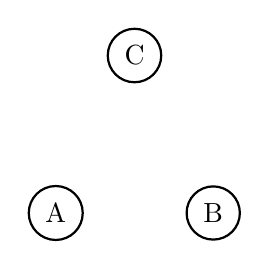
\begin{tikzpicture}
			\begin{scope}[every node/.style={circle,thick,draw}]
				\node (A) at (0,0) {A};
				\node (B) at (2,0) {B};
				\node (C) at (1,2) {C};
			\end{scope}
			
			\begin{scope}
				%\path (A) edge node {} (B);
				%\path (B) edge node {} (C);
				%\path (C) edge node {} (A);
			\end{scope}
		\end{tikzpicture}
		\caption{003 configuration}
	\end{subfigure}
	\hfill
	\begin{subfigure}[b]{0.2\linewidth}
		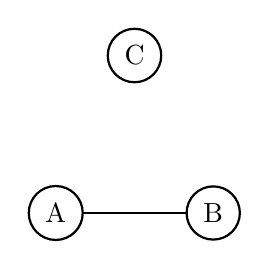
\begin{tikzpicture}
			\begin{scope}[every node/.style={circle,thick,draw}]
				\node (A) at (0,0) {A};
				\node (B) at (2,0) {B};
				\node (C) at (1,2) {C};
			\end{scope}
			
			\begin{scope}
				\path (A) edge node {} (B);
				%\path (B) edge node {} (C);
				%\path (C) edge node {} (A);
			\end{scope}
		\end{tikzpicture}
		\caption{102 configuration}
	\end{subfigure}
	\hfill
	\begin{subfigure}[b]{0.2\linewidth}
		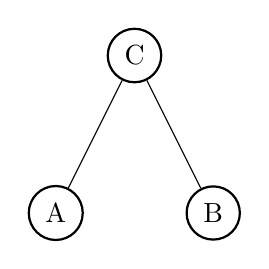
\begin{tikzpicture}
			\begin{scope}[every node/.style={circle,thick,draw}]
				\node (A) at (0,0) {A};
				\node (B) at (2,0) {B};
				\node (C) at (1,2) {C};
			\end{scope}
			
			\begin{scope}
				%\path (A) edge node {} (B);
				\path (B) edge node {} (C);
				\path (C) edge node {} (A);
			\end{scope}
		\end{tikzpicture}
		\caption{201 configuration}
	\end{subfigure}
	\hfill
	\begin{subfigure}[b]{0.2\linewidth}
		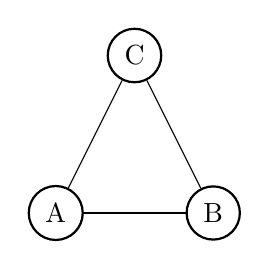
\begin{tikzpicture}
			\begin{scope}[every node/.style={circle,thick,draw}]
				\node (A) at (0,0) {A};
				\node (B) at (2,0) {B};
				\node (C) at (1,2) {C};
			\end{scope}
			
			\begin{scope}
				\path (A) edge node {} (B);
				\path (B) edge node {} (C);
				\path (C) edge node {} (A);
			\end{scope}
		\end{tikzpicture}
		\caption{300 configuration}
	\end{subfigure}
	\label{fig:triadic_structures}
	\caption{Possible triadic structures for any three nodes $A,B,C$.}
\end{figure}

\begin{table}
	\begin{tabularx}{\linewidth}{XXXXX}
		\hline
		\textbf{Dataset} & \textbf{Degree centrality} & \textbf{Betweenness centrality} & \textbf{Pagerank centrality} & \textbf{Connected components} \\
		\hline
		Yunnan & $1.3\pm3.2$ & $0\pm0$ & $0.0058\pm0.0055$ & $3/18$ \\
		Hainan & $1.5\pm1.8$ & $0\pm0$ & $0.0062\pm0.0043$ & $10/27$ \\
		Shaanxi & $0.99\pm1.3$ & $0\pm$ & $0.0042\pm0.0035$ & $12/40$ \\
		Xi'an & $0.7\pm1.4$ & $3.4\pm50.6$ & $0.0005\pm0.0006$ & $82/1291$\\
		\hline
	\end{tabularx}
	\caption{Network statistics for the Yunnan, Hainan, Shaanxi and Xi'an datasets. Values for centrality measures are mean value and standard deviation. Values for connected components are the number of connected components that are comprised of more than three nodes, and the total number of connected components.}
	\label{tab:network_stats}
\end{table}

\section{China Dataset}
\label{sec:china_data}

\paragraph{Dataset overview} This dataset contains COVID case information from all of China \cite{china_publication,china_data}. After preprocessing, there are 25,877 entries, with dates ranging from 2020-01-01 to 2022-08-14; therefore, this set is significantly larger than the ones discussed previously, and covers most of the pandemic. Relevant patient covariates are age, gender, residence, the location and/or activity where the patient was most likely infected, the patient's symptoms, the severity of the symptoms, and where the patient was registered by health authorities; covariates are also listed in \ref{tab:china_covariates}. The number of recorded covariates makes this dataset stand out among the others.

Out of the 25,877 confirmed cases, 20,577 have named no contacts at all, 2,995 have named one contact, 1,045 have named two contacts, and 1,260 have named three contacts or more. The mean age of patients is $42\pm18$ (information missing for 6,206 entries), with a 25 percentile of 30 and a 75 percentile of 54, meaning this dataset contains members of all age groups. 9,070 women versus 11,182 men shows a slight bias towards men (information missing for 5,625 entries). The three most common places of residence are \emph{Xi'an} (1,947), \emph{Wuhan} (1,671), and \emph{Shijiazhuang} (888) (information missing for 9,077 entries). The three most common occasions where patients were most likely infected are \emph{travel to Wuhan} (596), \emph{dinner} (360), and \emph{residence in Wuhan} (337) (information missing for 18,167 entries). The three most common symptoms are \emph{somatosensory related} (1,904), \emph{respiratory system/somatosensory related} (640), and \emph{respiratory system related} (495) (information missing for 20,142 entries). Out of the 7,061 cases where this information is available, 3,979 are classified as stable, 2,545 have mild symptoms, 405 have light symptoms, and 132 have severe symptoms. The three most common places of admission, i.e. where the patient was registered/admitted to hospital are \emph{Xi'an} (2292), \emph{Shanghai} (2079), and \emph{Guangzhou} (1398).

\begin{table}
	\begin{tabularx}{\linewidth}{XXX}
		\hline
		\textbf{Covariate} & \textbf{Description} & \textbf{Mean / Ratio / Range}\\
		\hline
		Date & Date when the case was confirmed/reported & 20/01/01 - 22/08/14\\
		Gender & Male/Female & $55.2\%$ \\
		Age & In years & $42\pm18$ \\
		Place of residence & - & -\\
		Place and event & Activity where infection might have happened & - \\
		Symptom & The patient's symptoms & - \\
		Symptom severity & - & - \\
		Place of admission & Where the patient was recorded by health authorities & - \\
		\hline
	\end{tabularx}
	\caption{Relevant covariates for the China dataset}
	\label{tab:china_covariates}
\end{table}

\paragraph{Network analysis} To the knowledge of the author, this dataset had not been analysed yet at the time of writing this.

\paragraph{A note on data quality} This dataset was compiled from 291 different data sources and although Liu et al. did a splendid job in standardising and coding the included variables, it's likely there are still some inconsistencies present in the data even after preprocessing, e.g. city names being written slightly different (Xi'an, Xian) and thus producing two unique values instead of one. Still, this should only be true for a negligible fraction of data entries, and thus not impact results in a significant manner.

\section{Bucharest Dataset}
\label{sec:bucharest_dataset}

\paragraph{Dataset overview} This dataset contains COVID case information from Bucharest, the capital of Romania \cite{bucharest_data}. It consists of 46,269 positively tested patients, of which 6,895 named at least one other person as a possible contact. Out of the 13,272 individuals nominated as contacts, 1,811 were themselves recorded as patients; therefore, this dataset differs from the others in the sense that not all named contacts were tested positive. Dates range from 2020-03-07 to 2020-11-11. Patient covariates deemed relevant are age, sex, the patient's field of work and whether the patient is active in the medical field; these are also listed in table \add{table, reference}. Out of the 46,269 positive cases and the additional 11,461 individuals who were nominated as contacts but were not themselves recorded as patients, 38,122 individuals have named no contacts at all, 15,856 have nominated one contact, 2,130 have nominated two contacts, and 1,727 patients have named three contacts or more \add{numbers don't add up, not sure why}. 

The average age of patients is $41\pm19$, with a 25 percentile of 29 and a 75 percentile of 53, meaning most are on the younger side. 21,665 males versus 24,604 females shows a slight bias towards females. Of the 6,964 patients where this information was recorded, only 186 are active in the medical field. Furthermore, a majority of patients for whom job information was recorded are not active in the labour market (6,298 out of 9,806). 

\begin{table}
	\begin{tabularx}{\linewidth}{XXX}
		\hline
		\textbf{Covariate} & \textbf{Description} & \textbf{Mean / Ratio / Range}\\
		\hline
		Date & Date when the case was confirmed/reported & 20/03/07 - 20/11/11\\
		Gender & Male/Female & $46.8\%$ \\
		Age & In years & $41\pm19$ \\
		Medical field & Whether the individual works in the medical sector & $2.7\%$ \\
		Active & Whether the individual is active in the labour market & $64.2\%$ \\
		\hline
	\end{tabularx}
	\caption{Relevant covariates for the Bucharest dataset}
	\label{tab:bucharest_covariates}
\end{table}

\paragraph{Network analysis} This dataset was analysed by H\^ancean et al. in two separate papers, with the first focusing on the role of age \cite{hancean2021role}, and the second addressing the impact of occupations on the spread of COVID-19 \cite{hancean2022occupations}.

\bigskip

In the first article, the authors combined patient covariates and certain network statistics into a relational hyperevent model (discussed in detail in section \ref{ch:methods}), which was then used to determine the impact of these variables on the likelihood of contact nominations. Specifically, they investigated age homophily, i.e. the average age difference between contact nominator (called \emph{referee} in the original paper) and nominees (called \emph{referrals} in the original paper); the average age of nominated contacts; sex homophily, i.e. the average sex difference between contact nominator and nominees; the average sex of nominated contacts; individual contact popularity, i.e. how often an individual is named as a contact; joint contact popularity, i.e. how often a pair of individuals have been named as contacts together; reciprocation, i.e. for any possible case contact nomination, where $i$ names $\{j,k,...,n\}$ as contacts at time $t_x$, how many individuals from $\{i,j,...,k\}$ have themselves named $i$ as a contact at a previous time $t_{x-y}$; contact activity, i.e. the number of contacts an individual has nominated before; nominations among contacts, i.e. for any possible case contact nomination, where $i$ names $\{j,k,...,n\}$ as contacts at time $t_x$, how many pairs of individuals $(j,k) \in \{j,k,...,n\}$ were involved in a contact nomination, where $j$ names $k$ as a contact, at a previous time $t_{x-y}$; and shared referee, i.e. for any possible case contact nomination, where $i$ names $\{j,k,...,n\}$ as contacts at time $t_x$, how many individuals from $\{j,k,...,n\}$ were named as contacts together with $i$ at a previous time $t_{x-y}$.

H\^ancean et al. reported the following results. The age difference between nominator and nominees is negatively associated with contact nomination likelihood, i.e. for any possible case contact nomination, where $i$ names $\{j,k,...,n\}$ as contacts, the likelihood of that contact nomination decreases with an increasing age discrepancy between nominator $i$ and nominees $\{j,k,...,n\}$; thus, there is age homophily, meaning that patients are likely to nominate contacts with an age similar to themselves. The average age of nominees is negatively associated with contact nomination likelihood, i.e. for any possible case contact nomination, where $i$ names $\{j,k,...,n\}$ as contacts, the likelihood of that contact nomination decreases with an increasing average age of the nominees $\{j,k,...,n\}$; this means that younger people are more likely to be nominated as contacts. The sex difference between nominator and nominees is positively associated with contact nomination likelihood, i.e. for any possible case contact nomination, where $i$ names $\{j,k,...,n\}$ as contacts, the likelihood of that contact nomination increases with an increasing degree of sex discrepancy between nominator $i$ and nominees $\{j,k,...,n\}$; thus, there is sex heterophily, meaning that patients are likely to nominate contacts of the opposite sex. Finally, the average sex of nominees is positively associated with contact nomination likelihood, i.e. for any possible case contact nomination, where $i$ names $\{j,k,...,n\}$ as contacts, the likelihood of that contact nomination increases with an increasing ratio of women in the nominee set $\{j,k,...,n\}$ (this is because sex was coded as male = 1 and female = 2; therefore, a higher average value across the nominee set means a higher fraction of nominees is female, while a lower average value would mean there are more males); this means that women are more likely to be nominated as contacts.

As for the network effects, the authors report these results. Individual contact popularity is negatively associated with contact nomination likelihood, i.e. for any possible case contact nomination, where $i$ names $\{j,k,...,n\}$ as contacts at time $t_x$, the likelihood of that contact nomination decreases with an increasing number of times individuals $\in \{j,k,...,n\}$ have already been named as contacts at previous times $t_{x-y}$; this means that individuals are unlikely to be named as a contact multiple times, although the authors note this is due to the nature of the dataset, where actors are very unlikely to appear more than once. Joint contact popularity is positively associated with contact nomination likelihood, i.e. for any possible case contact nomination, where $i$ names $\{j,k,...,n\}$ as contacts at time $t_x$, the likelihood of that contact nomination increases with an increasing number of pairs $(j,k) \in \{j,k,...,n\}$ who have been co-named as contacts in a previous contact nomination at time $t_{x-y}$; this means that people who are socially close are more likely to be nominated as contacts. Reciprocation is positively associated with contact nomination likelihood, i.e. for any possible case contact nomination, where $i$ names $\{j,k,...,n\}$ as contacts at time $t_{x}$, the likelihood of that contact nomination increases with an increasing number of individuals $\in \{j,k,...,n\}$ who have themselves nominated $i$ as a contact in a previous contact nomination at time $t_{x-y}$. This means nominated contacts tend to "return the favour". Contact activity is negatively associated with contact nomination likelihood, i.e. for any possible case contact nomination, where $i$ names $\{j,k,...,n\}$ as contacts at time $t_x$, the likelihood of that contact nomination decreases with an increasing number of contacts nominated by individuals $\in \{j,k,...,n\}$ in previous contact nominations at times $t_{x-y}$; this means that individuals who have previously acted as nominators are less likely to be named as contacts themselves later, which is again attributed to the nature of the dataset (see individual contact popularity). Nominations among contacts is positively associated with contact nomination likelihood, i.e. for any possible case contact nomination, where $i$ names $\{j,k,...,n\}$ as contacts at time $t_x$, the likelihood of that contact nomination increases with an increasing number of pairs $(j,k) \in \{j,k,...,n\}$ who were involved in a previous contact nomination at time $t_{x-y}$, where $j$ was the nominator and $k$ one of the nominees. This means that socially close individuals are more likely to be nominated as contacts together, in a similar fashion to joint contact popularity. Finally, shared referee is positively associated with contact nomination likelihood, i.e. for any possible case contact nomination, where $i$ names $\{j,k,...,n\}$ as contacts at time $t_x$, the likelihood of that contact nomination increases with an increasing number of individuals $j \in \{j,k,...,n\}$ who have been involved in a previous contact nomination at time $t_{x-y}$, where $i$ and $j$ were named as contacts together. This again hints at the influence of social closeness \cite{hancean2021role}.

\bigskip

In the second article, H\^ancean et al. analysed the dataset again, in a similar fashion, this time placing the focus on the role of occupations in the spread of COVID-19. For this, they added the following patient covariates to the model. Whether the individual was unemployed at the time of registration; whether the individual was employed in the private or public sector; whether the individual was employed in the medical sector; whether the individual was active in the labour market, i.e. either employed or employable; and the individual's age group, i.e. minor, adult, or pensioner.

Specifically, the authors investigated age homophily; the average age of nominated contacts; the age of the nominator; sex homophily; the average sex of nominated contacts; the sex of the nominator; the fraction of nominees active in the public sector; whether the nominator is active in the public sector; the fraction of nominees active in the medical sector; whether the nominator is active in the medical sector; active working force difference, i.e. the fraction of nominees who are either employed or employable, compared to whether the nominator is active in the workforce or not; the fraction of active nominees; whether the nominator is active in the workforce; individual contact popularity; joint contact popularity; reciprocation; in-degree of the nominator, i.e. for any possible contact nomination, where $i$ names $\{j,k,...,n\}$ as contacts at time $t_x$, how many times the nominator has himself been named as a contact at a previous time $t_{x-y}$; out-degree of the nominees, i.e. for any possible contact nomination, where $i$ names $\{j,k,...,n\}$ as contacts at time $t_x$, how many times contacts $j \in {j,k,...,n}$ have themselves acted as contact nominators at a previous time $t_{x-y}$; nominations among contacts; and shared referee;

The following results were reported regarding patient covariates. Nominator age is positively associated with contact nomination likelihood, i.e. for any possible contact nomination, where $i$ names $\{j,k,...,n\}$ as contacts, the likelihood of that contact nomination increases with an increasing age of $i$; this means that older people are more likely to contract COVID-19 and appear as nominators. There is no significant effect of the average age of nominees on contact nomination likelihood, i.e. for any possible contact nomination, where $i$ names $\{j,k,...,n\}$ as contacts, the average age of $\{j,k,...,n\}$ does not influence the likelihood of that contact nomination. The age difference between nominator and nominees is negatively associated with contact nomination likelihood, i.e. for any possible contact nomination, where $i$ names $\{j,k,...,n\}$ as contacts, the likelihood of that contact nomination decreases with an increasing age discrepancy between nominator $i$ and nominees $\{j,k,...,n\}$; thus, there is age homophily, as was found in the first paper. Nominator sex is positively associated with contact nomination likelihood when not controlling for network effects, i.e. for any possible contact nomination, where $i$ names $\{j,k,...,n\}$ as contacts, the likelihood of that contact nomination increases with if $i$ is female. The average sex of nominees is positively associated with contact nomination likelihood, i.e. for any possible contact nomination, where $i$ names $\{j,k,...,n\}$ as contacts, the likelihood of that contact nomination increases with an increasing ratio of women in the nominee set $\{j,k,...,n\}$ (again, sex was coded as male = 1 and female = 2); this means that women are more likely to be nominated as contacts, corroborating the authors' previous findings. The sex difference between nominator and nominees is positively associated with contact nomination likelihood, i.e. for any possible contact nomination, where $i$ names $\{j,k,...,n\}$ as contacts, the likelihood of that contact nomination increases with an increasing degree of sex discrepancy between nominator $i$ and nominees $\{j,k,...,n\}$; thus, there is sex heterophily, as was in the preceding article. Whether the nominator is working in the public sector is negatively associated with contact nomination likelihood, i.e. for any possible contact nomination, where $i$ names $\{j,k,...,n\}$ as contacts, the likelihood of that contact nomination decreases if the nominator $i$ works in the public sector; this means that people active in the public sector are less likely to contract COVID-19 and appear as nominators. The fraction of nominees working in the public sector is negatively associated with contact nomination likelihood, i.e. for any possible contact nomination, where $i$ names $\{j,k,...,n\}$ as contacts, the likelihood of that contact nomination decreases with an increasing number of nominees who are active in the public sector; this means that people who work in the public sector are also less likely to be named as contacts. Whether the nominator is active in the medical sector has no significant effect on contact nomination likelihood. The fraction of nominees active in the medical sector is negatively associated with contact nomination likelihood, i.e. for any possible contact nomination, where $i$ names $\{j,k,...,n\}$ as contacts, the likelihood of that contact nomination decreases with an increasing number of nominees who are active in the medical sector; this means that people who work in the medical sector are less likely to be named as contacts.  Whether the nominator is active in the workforce is positively associated with contact nomination likelihood, while the fraction of nominees who are active in the workforce is negatively associated with contact nomination likelihood, i.e. for any possible contact nomination, where $i$ names $\{j,k,...,n\}$ as contacts, the likelihood of that contact nomination increases if the nominator $i$ is active in the workforce, and decreases with an increasing number of nominees $\{i,j,...,k\}$ who are active in the workforce; this means that being either employed or employable increases the chance to contract COVID-19 and appear as a nominator, and decreases the chance to be named as contact. Accordingly, the active working force difference is positively associated with contact nomination likelihood, i.e. for any possible contact nomination, where $i$ names $\{j,k,...,n\}$ as contacts, the likelihood of that contact nomination increases with an increasing discrepancy of being active in the workforce between nominator $i$ and nominees $\{j,k,...,n\}$; this means that active people are more likely to nominate non-active individuals as contacts, and thus, there is an anti-homophily. 

As for the network effects, results were the following. Individual contact popularity is negatively associated with contact nomination likelihood; joint contact popularity is positively associated with contact nomination likelihood; reciprocation is positively associated with contact nomination likelihood; nominations among contacts is positively associated with contact nomination likelihood; shared referee is positively associated with contact nomination likelihood. These results corroborate findings from the previous article, and thus, interpretations are equivalent. Both the in-degree of the nominator and the out-degree of the nominees are negatively associated with contact nomination likelihood, i.e. for any possible contact nomination, where $i$ names $\{j,k,...,n\}$ as contacts at time $t_x$, the likelihood of that contact nomination decreases with an increasing number of previous contact nominations at a time $t_{x-y}$, where $i$ was named as a contact, and also decreases with an increasing number of previous contact nominations at a time $t_{x-y}$, where an individual $j \in \{j,k,...,n\}$ acted as a nominator \cite{hancean2021role,hancean2022occupations}. 

%\paragraph{A note on data availability and ethical considerations} Although a fair number of research on the topic of contact tracing data have been published (e.g. \add{CITE}), general data availability was rather restricted at the time of writing this. Many datasets were either only available upon request to the respective author or outright unavailable, presumably due to privacy considerations. Some were even behind paywalls. Due to this, four of the five datasets used in this work originate from China, where such data is widely available and was regularly published by local health authorities during the pandemic. Since all data records have been pseudonymised, there should be no ethical concern regarding privacy violation.
	\chapter{4\quad Methodology}
\label{ch:methods}

\section{Social Networks}
\label{sec:social_networks}

\subsection{Fundamentals}
\label{sec:social_networks_fundamentals}

In sociological terms, a social network is a social structure that maps out the relationships or interactions among various entities such as individuals, groups, organizations, or even entire societies. These entities, often referred to as nodes or vertices, are connected by one or multiple types of interdependencies, such as friendship, kinship, common interest, financial exchange, likes, dislikes, knowledge, prestige, or any other meaningful interactions or relationships.

Social networks are often visualized as graphs, where nodes represent the entities, and the edges or links represent the relationships or interactions between them. The patterns of these links often provide meaningful insights into the nature of relationships, social behaviours, group dynamics, organizational structures, and much more. For example, these structures may reveal who influences whom within a group or which entities act as gatekeepers or bridges in the flow of information or resources.

The size and complexity of social networks can vary greatly. They can be as small and simple as a family network or as vast and complex as the network of internet users across the globe. It's crucial to note that in a social network, the emphasis is on the relationships between entities, not just the entities themselves.

Graph theory, a fundamental area of mathematics, has found significant application in the study of social networks. In the context of social networks, graph theory provides a robust mathematical structure and a rich toolkit for understanding and analysing these networks.

A graph in mathematics is a structure that encapsulates the idea of pairwise relationships between objects. A graph comprises vertices (or nodes) and edges (or links). An edge connects a pair of vertices, indicating a relationship between them. This simple but powerful concept fits perfectly with the idea of a social network where entities (vertices) and their relationships (edges) form the fabric of the network. To make a formal definition, a basic social network can be defined as a tuple $G = (V,E)$, where $V$ is the set of vertices, and $E \subseteq V \times V$ is the set of edges.

\bigskip
\noindent Social network analysis (SNA) often leverages graph theory in multiple ways:

\begin{itemize}
	\item Visualisation: Graph theory aids in visually representing social networks, enabling a clear understanding of the complex web of relationships.
	\item Measurement and Analysis: Graph theory provides various measures and metrics such as centrality, clustering coefficient, diameter, etc., which can quantify important aspects of social networks like prominence of entities, propensity of clustering, reachability, etc.
	\item Modelling and Prediction: Graph models can mimic the behaviour of real-world social networks, helping in predicting future trends, understanding the spread of information or epidemics, or identifying influential entities in the network.
	\item Community Detection: Algorithms derived from graph theory help to discover communities or clusters within networks, revealing groups of entities with densely packed relationships.
\end{itemize}

\noindent In summary, a social network is a social structure that portrays interactions or relationships among entities. These networks can be effectively represented, measured, analysed, and modelled using the concepts and tools provided by graph theory, which provides a powerful mathematical lens to understand the complex dynamics of social networks. 

\subsection{Application to COVID-19 case contact data}
\label{sec:social_networks_application}

As mentioned earlier, social networks can be used to model the social dynamics of pandemic situations. Recall the definition of a social network as a tuple $G = (V,E)$. All datasets analysed in this work adhere to the basic form (time, source, target), and additional covariates depending on the dataset in question. The time component can be discarded for now, as it becomes relevant only when working with relational (hyper)event models later on. In the context of case contact networks, $V$ therefore is the set of cases/contacts, and $E$ is the set of contact nominations between cases. One might make a case for using bipartite (also known as two-mode networks), where vertices are divided into two classes, and edges only exist between vertices of different class \cite{borgatti1997network,latapy2008basic}. Although it may seem sensible to do this here, where, in principle, there are indeed two classes (nominators and nominees), in practice, this only holds true for the data from Bucharest, where a large fraction of nominated contacts were never registered as positive cases. However, it is not clear if this is only due to missing information, i.e. they might have contracted the virus and health authorities were just not aware of it, or due to them indeed not having been infected. Therefore, and to ensure comparability of results, two-mode networks were not used to model the case contact networks here. 

Also, there is the question of directionality. Networks can be either directed or undirected, meaning that edges between nodes $u$ and $v$ are either one- or bidirectional. Directed networks usually carry a different semantic meaning compared to undirected ones, and also differ in the computation of network effects. For example, in a directed network, nodes have an in-degree and an out-degree, i.e. the number of incoming and outgoing edges, respectively; therefore, there also need to be two measures for degree centrality, one accounting for in-degree, and one for out-degree. Although it might seem sensible to use directed networks here, since contact nominations are of a (source, target) form, the actual semantic meaning of the connection is often not clear (i.e. whether the source node is naming possible contacts who might have infected him, or if the source node is naming contacts whom he himself might have infected) \cite{kojaku2021effectiveness}, except for the Bucharest dataset, where it is explicitly stated that authorities employed backward contact tracing, i.e. patients name individuals who might be the source of their infection \cite{hancean2021role}.

\subsection{Network analysis}
\label{sec:social_networks_analysis}

As mentioned in section \ref{sec:social_networks_fundamentals}, graph theory offers a wide array of methods to extract useful information from social networks. In the context of pandemics, key interests include the identification of influential individuals (e.g. "super-spreaders") and the overall dynamic of infections, i.e. in which patterns a virus tends to spread; insights into these factors help understanding, and therefore combatting the respective pandemic, e.g. by putting a particular focus on individuals who are similar to those found to be especially prone to spread the virus to others \add{cite}.

For all networks derived from the different datasets, the following network statistics were computed:

\begin{itemize}
	\item Degree centrality: For any node $v \in V$, the degree centrality is defined as $C_D(v) = \text{deg}(v)$, i.e. the degree centrality of a node is equal to the number of edges connected to that node. This measure can be used to identify individuals who hold an important position in the network (in this context, those who nominate many contacts), and also as an indicator for overall network density.
	\item Betweenness centrality: For any node $v \in V$, the betweenness centrality is defined as $C_B(v) = \sum_{s\neq v\neq t\in V}\frac{\sigma_{st}(v)}{\sigma_{st}}$, where $\sigma_{st}$ is the total number of shortest paths from $s$ to $t$, and $\sigma_{st}(v)$ is the number of shortest paths from $s$ to $t$ that go through $v$. This measure can be used to identify individuals who facilitate information flow (in this context, those who might have spread the virus from one individual to another).
	\item Pagerank centrality: This is an iterative algorithm originally proposed to rank websites according to importance, where importance is defined by the number of hyperlinks that point to that website. For any node $v \in V$, the pagerank centrality is defined as $C_P(v) = \sum_{u \in B_v}\frac{C_P(u)}{\text{deg}(u)}$, where $B_v$ is the set of all nodes connected to $v$. Pagerank is computed iteratively; at time 0, it is
	\begin{equation*}
		PR(v_i;0) = \frac{1}{N} \forall v_i \in V
	\end{equation*}
	where $N = \lvert V \rvert$. At time $t$, it is
	\begin{equation*}
		PR(v_i;t+1) = \frac{1 - d}{N} + d \sum_{v_j \in B_{v_i}} \frac{PR(v_j;t)}{deg(v_j)} \forall v_i \in V
	\end{equation*}
	where $d = 0.85$ is the damping parameter. This measure is another way to identify important individuals in the network.
	\item Component size: The task of community detection is the division of a network into a set of sub-networks according to specific criteria; in general, a community is a set of nodes with a strong cohesion, i.e. a high degree of inter-connectedness, while connections to other groups are sparse or even non-existent. Here, the latter is the case, i.e. a connected component is a set of nodes $C = \{v_1,...,v_n\} \in V$, where for each pair of nodes $v_i,v_j \in C$, there exists an edge $(v_i,v_j) \in E$, and for each pair $v_i,n_j;\: v_i \in C, n_j \in V \setminus C$, there is no edge, i.e. $(v_i,n_j) \notin E$. This division can be achieved e.g. by \emph{Markov clustering algorithm} \cite{community_detection,markov_clustering}. In the context of pandemics, community detection can be used to identify infection clusters. Therefore, connected components are computed for all networks, and component size is determined for all nodes.
	\item Average shortest path length: In general, the shortest path between any two nodes $v_x,v_y \in V$ is a sequence of vertices $S = (v_x,...,v_y)$ such that 
	\begin{enumerate}
		\item for all $v_i,v_j \in S, i < j$, there is an edge $(v_i,v_j) \in E$
		\item out of all possible paths between $v_x$ and $v_y$, $S$ has the smallest cost
	\end{enumerate}
	where cost is the sum of weights associated with the edges. Since the graphs here are unweighted, i.e. all edges have a weight value of 1, the shortest path amounts to that sequence $S$ that contains the lowest amount of nodes out of all possible sequences. Shortest paths can be computed for example by the Dijkstra or A* algorithm \add{cite dijsktra, a* and shortest path definition}. In the context of case contact networks, shortest paths yield interesting insights into transmission chains, and the average shortest path length of a network might be used as a measure for how effective containment methods (e.g. lockdowns, social distancing etc.) have been.
\end{itemize}  
\bigskip

\noindent Based on these statistics, the data was analysed both in qualitative and quantitative manner. Specifically, examples are given for how epidemiological insights can be gained from contact tracing data (qualitative), and the statistics computed for the different datasets are statistically compared to investigate whether there are significant differences between the different regions (quantitative). Results are presented in section \ref{ch:results_discussion}.

\section{Relational Event Models}
\label{sec:rem}

\subsection{Fundamentals}
\label{sec:rem_fundamentals}

Relational event models (REMs) are a class of statistical models used for analysing ordered sequences of social interactions among actors. They offer a means to explain the timing and sequencing of events in a social network context, often focusing on patterns of communication, relationships, and interactions between network actors over time. 

In the realm of social networks, an event signifies an action that happens at a specific point in time from one actor to another. For instance, in a network of email communications among a group of people, an email sent by person A to person B would be considered an event. REMs are concerned with the study of these actions or events, their timing, and the dependencies between them.

The main idea behind REMs is to treat social interactions as events that happen in continuous time, rather than at discrete, predetermined intervals. Each event in the sequence is an interaction between pairs of actors, and the time between consecutive events is explicitly modelled and analysed. 

\noindent REMs take into consideration two key factors:

\begin{enumerate}
	\item Order of events: The order in which events occur can have significant implications. For example, an email conversation would make little sense if the emails are not read in the sequence they were sent and received.
	\item Timing of events: The time between consecutive events can reveal crucial information. For example, the length of time between receiving an email and replying to it could indicate the importance or urgency of the conversation.
\end{enumerate}

REMs use the order and timing information to make inferences about the underlying social process that generated the observed sequence of events. They allow for the analysis of dynamic network data in ways that conventional social network analysis tools, which often assume static networks, can not. 

Applications of REMs include studying patterns of communication in social media, organisational behaviour, group dynamics, online collaboration, animal social behaviour, and many other fields where understanding the sequence and timing of interactions can provide valuable insights.

In essence, relational event models specify the probability of a possible event sequence $E$ happening up to a point in time $t_n$, given a sequence of past events $E_{<t_n}$; formally, it is
\begin{equation*}
	P(E) = \prod_{i=1}^{n}P(e_i|E_{<t_i})
\end{equation*}
where $E = (e_1,...,e_n)$ is a sequence of events, and $E_{<t_i} = \{e_j \in E;\: t_j < t_i\}$ is the sequence of past events before $t_i$.

The partial likelihood for a specific event $e_i = (u_i,v_i,t_i)$, which is an interaction from $u_i$ to $v_i$ ($u_i,v_i \in A$, i.e. $A = U \cup V$ is the set of all actors; $U$ and $V$ are the not necessarily disjoint sets of sources and targets) is expressed in terms of hazard functions. It is
\begin{equation*}
	P(e_i|E_{<t_i};\theta) = \frac{\lambda(u_i,v_i,t_i;\theta)}{\sum_{uv\in R_{t_i}}\lambda(u,v,t_i;\theta)}
\end{equation*}
where $\lambda(u,v,t_i;\theta)$ is the hazard rate of the dyad $(u,v)$, i.e. the expected number of events on $(u,v)$ per time unit, and $R_{t_i}$ is the set of all events that could potentially happen at time $t_i$, aka the risk set. The rate function $\lambda$ depends on source ($u$), target ($v$), event type, past event history ($E_{<t_i}$), and exogenous variables. It is given by
\begin{align*}
	\lambda(u,v,t_i;\theta) = \lambda_0(t_i) \cdot \lambda_1(u,v,t_i;\theta)
\end{align*}
i.e. it is decomposed into an arbitrary baseline rate $\lambda_0$ and a parametrised relative rate $\lambda_1$:
\begin{align*}
	\lambda_1(u,v,t_i;\theta) &= \exp(\theta^T s(u,v;E_{<t_i}))\\
	&= \exp(\sum_h \theta_h \cdot s_h(u,v;E_{<t_i}))&&
\end{align*}
This is expressed by a vector of statistics $s$, which is parametrised by a vector of unknown parameters ($\theta$, estimated from the data), which determine the influence of each individual factor on the overall incidence rate. To summarise, the probability for a particular event $e_i$ occurring is the hazard rate of $e_i$ divided by the sum of the hazard rates of all events which could potentially occur at time $t_i$ \cite{butts20084}.

The statistics expressed by $s$ may be broadly categorised into endogenous and exogenous factors; endogenous factors are derived from past events involving $u$ and $v$, and possibly common third actors, while exogenous factors are given by covariates specific to the actors, e.g. personal characteristics like age or sex. 

Given a set of sufficient statistics $s$, the model parameters $\theta$ can be determined through maximum likelihood estimation (MLE), such that \[\hat{\theta} = \argmax_{\theta} P(E|\theta)\]

A potential issue in this MLE is the computation of the risk set $R$; this is because the number of potential events occurring at time $t_i$ rises quadratically with the number of actors (with $N$ actors, for each time step $t_i$, there are $N \cdot (N - 1)$ possible events) \cite{butts20084}. This can be alleviated by replacing the full risk set $R_{t_i}$ by a sampled risk set $\tilde{R_{t_i}}$, which contains an arbitrary number of potential events per observed event (e.g. 100 potential, but unobserved events per every one event seen in the data), which are sampled uniformly at random \cite{eventnet_rem}.

\subsection{Application to COVID-19 case contact data}
\label{sec:rem_application}

Recall that all case contact datasets conform to the basic format (timestamp, source, target). Therefore, they are, in essence, sequences of events, where the social interaction between the actors is a contact nomination. Conventional social network analysis, as described in section \ref{sec:social_networks}, neglects the time component of the data entirely. Therefore, it seems prudent to also analyse the data using relational event modelling. It is worthy to note that, in contrast to static network modelling, REM necessitates an assumption of directionality, i.e. events have a source and a target; in this case, the source would be the nominator, and the target the nominee. However, the fact remains that it is difficult to determine the actual semantic of a particular interaction, i.e. whether the source infected the target, or vice versa.

As mentioned before, there are essentially two steps, which are 1) the computation of statistics $s$, and 2) the estimation of model parameters $\theta$. Therefore, it is necessary to specify a set of statistics which may potentially influence the incidence rate of events. Based on previous work (\cite{butts20084,brandes2009networks,stadtfeld2017interactions}), the following effects were analysed:

\begin{figure}
	\centering
	\begin{subfigure}[t]{0.2\linewidth}
		\vskip 0pt
		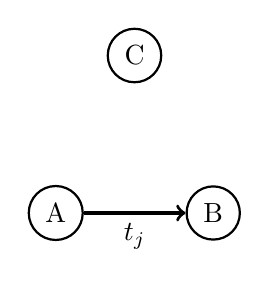
\begin{tikzpicture}
			\begin{scope}[every node/.style={circle,thick,draw}]
				\node (A) at (0,0) {A};
				\node (B) at (2,0) {B};
				\node (C) at (1,2) {C};
			\end{scope}
			
			\begin{scope}[every edge/.style={draw=black,very thick}]
				\path [->] (A) edge node [below] {$t_j$} (B);
				%\path (B) edge node {} (C);
				%\path (C) edge node {} (A);
			\end{scope}
		\end{tikzpicture}
		\caption{Event $(A,B,t_j)$}
	\end{subfigure}
	\hfill
	\begin{subfigure}[t]{0.2\linewidth}
		\vskip 0pt
		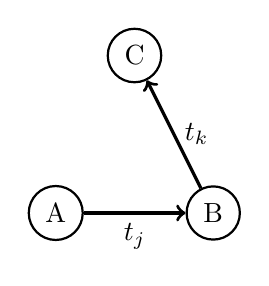
\begin{tikzpicture}
			\begin{scope}[every node/.style={circle,thick,draw}]
				\node (A) at (0,0) {A};
				\node (B) at (2,0) {B};
				\node (C) at (1,2) {C};
			\end{scope}
			
			\begin{scope}[every edge/.style={draw=black,very thick}]
				\path [->] (A) edge node [below] {$t_j$} (B);
				\path [->] (B) edge node [right] {$t_k$} (C);
				%\path (C) edge node {} (A);
			\end{scope}
		\end{tikzpicture}
		\caption{Event $(B,C,t_k)$}
	\end{subfigure}
	\hfill
	\begin{subfigure}[t]{0.2\linewidth}
		\vskip 0pt
		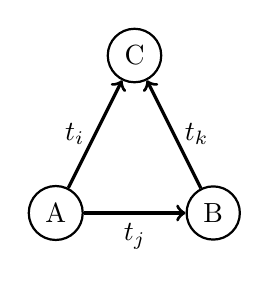
\begin{tikzpicture}
			\begin{scope}[every node/.style={circle,thick,draw}]
				\node (A) at (0,0) {A};
				\node (B) at (2,0) {B};
				\node (C) at (1,2) {C};
			\end{scope}
			
			\begin{scope}[every edge/.style={draw=black,very thick}]
				\path [->] (A) edge node [below] {$t_j$} (B);
				\path [->] (B) edge node [right] {$t_k$} (C);
				\path [->] (A) edge node [left] {$t_i$} (C);
			\end{scope}
		\end{tikzpicture}
		\caption{Transitive closure through event $(A,C,t_i)$}
	\end{subfigure}
	\hfill
	\begin{subfigure}[t]{0.2\linewidth}
		\vskip 0pt
		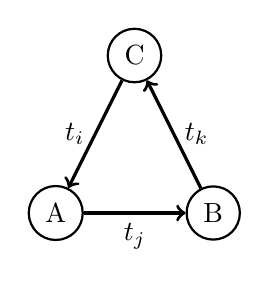
\begin{tikzpicture}
			\begin{scope}[every node/.style={circle,thick,draw}]
				\node (A) at (0,0) {A};
				\node (B) at (2,0) {B};
				\node (C) at (1,2) {C};
			\end{scope}
			
			\begin{scope}[every edge/.style={draw=black,very thick}]
				\path [->] (A) edge node [below] {$t_j$} (B);
				\path [->] (B) edge node [right] {$t_k$} (C);
				\path [->] (C) edge node [left] {$t_i$} (A);
			\end{scope}
		\end{tikzpicture}
		\caption{Cyclical closure through event $(C,A,t_i)$}
	\end{subfigure}
	\caption{Illustration of transitive and cyclical closure in relational event models. Time ordering is $t_j < t_k < t_i$.}
	\label{fig:rem_closure}
\end{figure}

\begin{itemize}
	\item Effects depending on past events:
	\begin{itemize}
		\item Nomination activity, i.e. the influence of the number of past events at times $<t_i$ involving actor $u$ as a source on the likelihood a possible event $(u,v,t_i)$ $\rightarrow$ is the nomination activity of $u$ associated with the likelihood of a future event on the dyad $(u,v)$?
		\begin{align*}
			&nomination.activity(e(u,v,t_i)) = \sum_{v' \in V} e(u,v',<t_i)&&\\
			&nomination.activity(e(u,v,t_i)) = \lvert E' \rvert; E' = \{e(u,v',t_j) \forall v' \in V \land t_j < t_i\}
		\end{align*}
		\item Exact repetition, i.e. the influence of the number of past events $(u,v,<t_i)$ on the likelihood of a possible event $(u,v,t_i)$ $\rightarrow$ is the likelihood of a future event on the dyad $(u,v)$ associated with the number of past observed events on the same dyad?
		\begin{align*}
			exact.repetition(e(u,v,t_i)) = \sum e(u,v,<t_i)
		\end{align*}
		\item Reciprocation, i.e. the influence of the number of past events $(x,u,<t_i)$ on the likelihood of a possible event $(u,v,t_i)$ $\rightarrow$ is the number of times $u$ has been named as a contact in the past associated with the likelihood of a future event on the dyad $(u,v)$, i.e. $u$ now acting as a nominator himself?
		\begin{align*}
			reciprocation(e(u,v,t_i)) = \sum_{u' \in U} e(u',u,<t_i)
		\end{align*}
		\item Exact reciprocation, i.e. the influence of the number of past events $(v,u,<t_i)$ on the likelihood of a possible event $(u,v,t_i)$ $\rightarrow$ is the number of past events on the dyad $(v,u)$ associated with the likelihood of a future event involving the same actors, but with roles reversed?
		\begin{align*}
			exact.reciprocation(e(u,v,t_i)) = \sum e(v,u,<t_i)
		\end{align*}
		\item Transitive tie, i.e. the influence of past events $(u,x,t_j)$ and $(x,v,t_k)$, $j < k < i$ on the likelihood of a possible event $(u,v,t_i)$ $\rightarrow$ is there a tendency for transitive closure?
		\begin{align*}
			transitive.tie(e(u,v,t_i)) = \sum_{x=1}^{\lvert \mathcal{R} \rvert} \min [d(u,x,A_{t_i}), d(x,v,A_{t_i})]
		\end{align*}
		($\mathcal{R}$ is the set of potential targets; $d(x,y,A_{t_i})$ is the accumulated volume of interactions from $x$ to $y$ by the time $t_i$)
		\item Cyclical tie, i.e. the influence of past events $(u,x,t_j)$ and $(x,v,t_k)$, $j < k < i$ on the likelihood of a possible event $(v,u,t_i)$ $\rightarrow$ is there a tendency for cyclical closure? (for an illustration, refer to figure \ref{fig:rem_closure})
		\begin{align*}
			cyclical.tie(e(u,v,t_i)) = \sum_{x=1}^{\lvert \mathcal{R} \rvert} \min [d(v,x,A_{t_i}), d(x,u,A_{t_i})]
		\end{align*}
		\item Shared source, i.e. the influence of the number of past events $(x,u,t_j)$ and $(x,v,t_k)$, $j \leq k < i$ on the likelihood of a possible event $(u,v,t_i)$ or $(v,u,t_i)$ $\rightarrow$ is there a tendency for actors who have been nominated as contacts by the same individual to name each other as contacts at a later time? (for an illustration, refer to figure \ref{fig:rem_triangle_children})
		\begin{align*}
			shared.source(e(u,v,t_i)) = \sum_{x=1}^{\lvert \mathcal{R} \rvert} \min [d(x,u,A_{t_i}), d(x,v,A_{t_i})]
		\end{align*}
		\item Shared target, i.e. the influence of the number of past events $(u,x,t_j)$ and $(v,x,t_k)$, $j \leq k < i$ on the likelihood of a possible event $(u,v,t_i)$ or $(v,u,t_i)$ $\rightarrow$ is there a tendency for actors who have nominated the same individual as a contact to name each other as contacts at a later time? (for an illustration, refer to figure \ref{fig:rem_triangle_parents})
		\begin{align*}
			shared.sender(e(u,v,t_i)) = \sum_{x=1}^{\lvert \mathcal{R} \rvert} \min [d(u,x,A_{t_i}), d(v,x,A_{t_i})]
		\end{align*}
	\end{itemize}
	\item Effects depending on actor attributes:
	\begin{itemize}
		\item Nominator age
		\item Nominee age
		\item Age difference between nominator and nominee (age homophily)
		\item Nominator sex
		\item Nominee sex
		\item Sex difference between nominator and nominee (sex homophily)
		\item Other covariates specific to the individual datasets, which are listed in section \ref{ch:previous_work_data}. In general, there are three statistics for each covariate: the value of the nominator, the value of the nominee, and the difference between the values.
	\end{itemize}
\end{itemize}

\begin{figure}
	\centering
	\begin{subfigure}[t]{0.3\linewidth}
		\vskip 0pt
		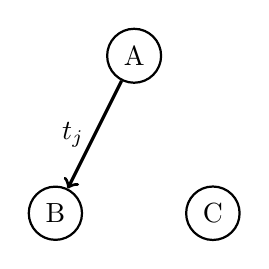
\begin{tikzpicture}
			\begin{scope}[every node/.style={circle,thick,draw}]
				\node (A) at (1,2) {A};
				\node (B) at (0,0) {B};
				\node (C) at (2,0) {C};
			\end{scope}
			
			\begin{scope}[every edge/.style={draw=black,very thick}]
				\path [->] (A) edge node [left] {$t_j$} (B);
				%\path (B) edge node {} (C);
				%\path (C) edge node {} (A);
			\end{scope}
		\end{tikzpicture}
		\caption{Event $(A,B,t_j)$}
	\end{subfigure}
	\hfill
	\begin{subfigure}[t]{0.3\linewidth}
		\vskip 0pt
		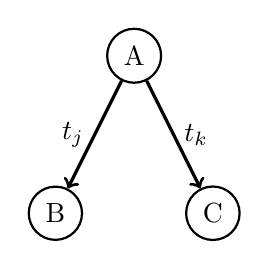
\begin{tikzpicture}
			\begin{scope}[every node/.style={circle,thick,draw}]
				\node (A) at (1,2) {A};
				\node (B) at (0,0) {B};
				\node (C) at (2,0) {C};
			\end{scope}
			
			\begin{scope}[every edge/.style={draw=black,very thick}]
				\path [->] (A) edge node [left] {$t_j$} (B);
				\path [->] (A) edge node [right] {$t_k$} (C);
				%\path (C) edge node {} (A);
			\end{scope}
		\end{tikzpicture}
		\caption{Event $(B,C,t_k)$}
	\end{subfigure}
	\hfill
	\begin{subfigure}[t]{0.3\linewidth}
		\vskip 0pt
		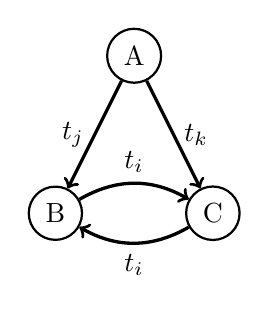
\begin{tikzpicture}
			\begin{scope}[every node/.style={circle,thick,draw}]
				\node (A) at (1,2) {A};
				\node (B) at (0,0) {B};
				\node (C) at (2,0) {C};
			\end{scope}
			
			\begin{scope}[every edge/.style={draw=black,very thick}]
				\path [->] (A) edge node [left] {$t_j$} (B);
				\path [->] (A) edge node [right] {$t_k$} (C);
				\path [->] (B) edge [bend left] node [above] {$t_i$} (C);
				\path [->] (C) edge [bend left] node [below] {$t_i$} (B);
			\end{scope}
		\end{tikzpicture}
		\caption{Shared source through event $(A,C,t_i)$}
	\end{subfigure}
	\hfill
	\caption{Illustration of shared source in relational event models. Time ordering is $t_j \leq t_k < t_i$.}
	\label{fig:rem_triangle_children}
\end{figure} 

\begin{figure}
	\centering
	\begin{subfigure}[t]{0.3\linewidth}
		\vskip 0pt
		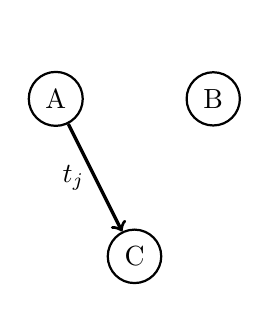
\begin{tikzpicture}
			\begin{scope}[every node/.style={circle,thick,draw}]
				\node (A) at (0,2) {A};
				\node (B) at (2,2) {B};
				\node (C) at (1,0) {C};
			\end{scope}
		
			\begin{scope}[every edge/.style={very thick}]
				\path [->] (A) edge [bend left] node [above,style={text opacity=0}] {$t_i$} (B);
				\path [->] (B) edge [bend left] node [below] {} (A);
			\end{scope}
			
			\begin{scope}[every edge/.style={draw=black,very thick}]
				\path [->] (A) edge node [left] {$t_j$} (C);
				%\path (B) edge node {} (C);
				%\path (C) edge node {} (A);
			\end{scope}
		\end{tikzpicture}
		\caption{Event $(A,B,t_j)$}
	\end{subfigure}
	\hfill
	\begin{subfigure}[t]{0.3\linewidth}
		\vskip 0pt
		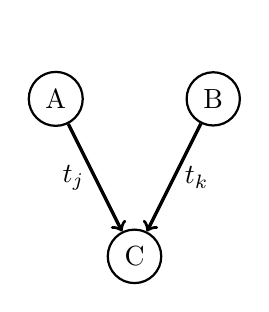
\begin{tikzpicture}
			\begin{scope}[every node/.style={circle,thick,draw}]
				\node (A) at (0,2) {A};
				\node (B) at (2,2) {B};
				\node (C) at (1,0) {C};
			\end{scope}
		
			\begin{scope}[every edge/.style={very thick}]
				\path [->] (A) edge [bend left] node [above,style={text opacity=0}] {$t_i$} (B);
				\path [->] (B) edge [bend left] node [below] {} (A);
			\end{scope}
			
			\begin{scope}[every edge/.style={draw=black,very thick}]
				\path [->] (A) edge node [left] {$t_j$} (C);
				\path [->] (B) edge node [right] {$t_k$} (C);
				%\path (C) edge node {} (A);
			\end{scope}
		\end{tikzpicture}
		\caption{Event $(B,C,t_k)$}
	\end{subfigure}
	\hfill
	\begin{subfigure}[t]{0.3\linewidth}
		\vskip 0pt
		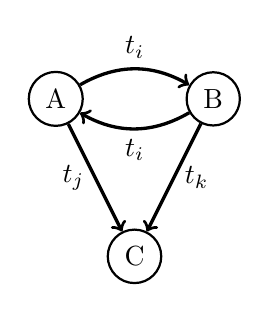
\begin{tikzpicture}
			\begin{scope}[every node/.style={circle,thick,draw}]
				\node (A) at (0,2) {A};
				\node (B) at (2,2) {B};
				\node (C) at (1,0) {C};
			\end{scope}
			
			\begin{scope}[every edge/.style={draw=black,very thick}]
				\path [->] (A) edge node [left] {$t_j$} (C);
				\path [->] (B) edge node [right] {$t_k$} (C);
				\path [->] (A) edge [bend left] node [above] {$t_i$} (B);
				\path [->] (B) edge [bend left] node [below] {$t_i$} (A);
			\end{scope}
		\end{tikzpicture}
		\caption{Shared target through event $(A,C,t_i)$}
	\end{subfigure}
	\hfill
	\caption{Illustration of shared target in relational event models. Time ordering is $t_j \leq t_k < t_i$.}
	\label{fig:rem_triangle_parents}
\end{figure}

These statistics were calculated using the \emph{eventnet} software \cite{eventnet_rem,eventnet_rhem} (step 1). Using the \emph{R} package \emph{survival} \cite{survival-package}, a Cox proportional hazards model was fitted on the result tables in order to estimate the model parameters $\theta$, and therefore draw conclusions regarding significance and effect of the individual statistics (step 2). Results are presented and discussed in chapter \ref{ch:results_discussion}.

\section{Relational Hyperevent Models}
\label{sec:rhem}

\subsection{Fundamentals}
\label{sec:rhem_fundamentals}

A limiting factor for relational event modelling is the restriction to dyadic interactions; while many events involve not only two but multiple actors (e.g. an email sent to a mailing list containing multiple recipients), these events are treated independently of one another in REM. This negligence of possible dependencies between targets may lead to erroneous parameter estimations. For example, take a possible event $(A,B,t_i)$, where Alice sends an email to Bob at time $t_i$. There is also a history of past interactions $(A,B,t_j)$ and $(A,C,t_j); t_i < t_j$, where Alice sent an email addressing both Bob and Charlie. A relational event model containing a \emph{repetition} statistic would find a positive effect for this interaction, while in reality, Alice might always send emails addressed to both Bob and Charlie, but never to Bob alone, so an event $(A,B,t_i)$ would actually be a novelty instead of a repetition. 

Perry and Wolfe \cite{perry2013point} propose an adjusted formula for the intensity rate
\begin{align*}
	&\lambda(u,J,t_i;\theta) = \lambda_0(t_i) \cdot \lambda_1(u,J,t_i;\theta)&&\\
	&\lambda_1(u,J,t_i;\theta) = \exp(\theta^T \sum_{j\in J} s(u,j;E_{<t_i})) \prod_{j\in J} \mathbf{1}\{j \in \mathcal{J}_{t_i} (u)\} \add{what is meant by last part?}&&
\end{align*}
where $u$ is the source of the interaction, $J$ is the set of targets of the interaction, and $\mathcal{J}_{t_i} (u)$ is the set of all possible targets of $u$ at time $t_i$. This model therefore assumes that covariate vectors $s$ of recipients $j \in J$ influence the intensity rate for an event $(u,J,t_i)$ independently of one another, since intensity of a multicast interaction is expressed through a decomposition into dyadic interactions \cite{perry2013point,lerner2021relational}.

Other approaches include the creation of artificial nodes that contain the receiver set (refer to figure \ref{fig:polyadic_interactions}) and the employment of hyperedge or latent variable models; issues with these are a possibly intractable amount of receiver set nodes in the first case, and limitation to dyadic functions in the latter two cases \cite{lerner2021relational}. 
\bigskip

\noindent Lerner et al \cite{lerner2019rem} propose a generalisation of relational event models based on hypergraphs. Hypergraphs are an extension of traditional graphs, where edges can not only connect two, but any number of nodes; formally, a hypergraph is defined by a tuple $H = (V, E)$, where $V$ is the set of vertices, and $E \subseteq 2^V$ is a set of non-empty subsets of $V$, i.e. the hyperedges. A directed hypergraph is defined by a triplet $H = (U,V,E)$, where $U$ (= sources) and $V$ (= targets) are sets of vertices, and $E \subseteq 2^U \times 2^V$ is a set of tuples $h = (u,v)$, where $u \in U$ is a non-empty set of source vertices, and $v \in V$ is a non-empty set of target vertices \cite{wang2018development,lerner2019rem}. Henceforth, only the directed case shall be considered.

Based on the concepts of REM, a directed hyperevent is given by $e_i = (h_i, t_i, x_i)$, where $h_i$ is a directed hyperedge, $t_i$ is a point in time when the event takes place, and $x_i$ is the type of the event (e.g. sending an email); the latter component will be neglected as it is not relevant to this work. Similarly, the hazard rate is given by
\begin{align*}
	&\lambda(h,t_i,\theta) = \theta_0(t_i) \cdot \lambda_1(h,t_i;\theta)&&\\
	&\lambda_1(h,t_i;\theta) = \exp(\theta^T s(h;E_{<t_i}))
\end{align*}
and the partial likelihood of an event sequence is given by 
\begin{align*}
	L(\theta) = \prod_{e \in E_{<t_i}} \frac{\lambda_1(h_e,t_e;\theta)}{\sum_{h\in R_{t_e}} \lambda_1(h,t_e;\theta)}
\end{align*}
Compared to the approach by Perry and Wolfe, the only difference is the substitution of the decomposition of statistic vectors $\sum_{j} s(u,j;E_{<t_i})$ for a hyperedge vector $s(h;E_{<t_i})$ \cite{lerner2019rem,lerner2021relational}. Apart from that, the computation of the risk set $R$ poses an even greater problem than it does for relational event models. This is because all possible hyperedges need to be considered, the number of which rises exponentially with the number of nodes. Like before, case-control sampling is used to reduce the risk set to a tractable size \cite{lerner2019rem,lerner2021relational}.
\bigskip

\noindent The main novelty, therefore, is the definition of the statistics $s$.

\subsection{Application to COVID-19 case contact data}
\label{sec:rhem_application}

Obviously, most contact nomination events are not dyadic, but polyadic, i.e. multiple actors are involved; think, for example, of a birthday party, after which one of the attendees tests positive and names all other guests as contacts. Therefore, conventional relational event models may fail to identify dynamics due to their dyadic nature. As stated in the previous section, a directed hyperevent generally consists of a non-empty set of source actors $u$ and target actors $v$; since in all datasets used in this work there is always a single COVID-19 patient nominating one or more contacts, it is $\lvert u \rvert$ for all hyperevents, i.e. there is only one source actor. For this reason, directed RHEM were chosen instead of undirected.

The statistics included in the models are in part similar to the ones used in REM, but differ in their definition. Once again, they can be divided into endogenous and exogenous effects, i.e. statistics depending on prior events, and statistics depending on actor covariates. Based on previous work (\cite{lerner2019rem,lerner2021relational,hancean2021role,hancean2022occupations}), the following were analysed:

\begin{itemize}
	\item Effects depending on past events:
	\begin{itemize}
		\item Nominee set size, i.e. the influence of the size of the target set of a hyperedge $h$ involved in past events $e(h,<t_i)$ at times $<t_i$ on the likelihood of a possible event $e(h,t_i)$ $\rightarrow$ is the number of named contacts associated with the likelihood of future events?
		\begin{align*}
			nominee.size(e(h,t_i)) = \lvert v \rvert; \: h = (u,v)
		\end{align*}
		\item Exact repetition, i.e. the influence of the number of past events $e(h,<t_i)$ on the likelihood of a possible event $e(h,t_i$) $\rightarrow$ is the number of past events on a hyperedge $h$ associated with the likelihood of a future event on the exact same hyperedge?
		\begin{align*}
			exact.repetition(e(h,t_i)) = \sum e(h,<t_i)
		\end{align*}
		\item Unordered repetition, i.e. the influence of the number of past events $e(h',<t_i)$ on the likelihood of a possible event $e(h,t_i)$, where $h' = (u',v'); \: h = (u,v); \: u',v' \in u \cup v$ $\rightarrow$ is the likelihood of a future event $e(h,t_i)$ associated with the number of past events on hyperedges which contain the same actors, but not necessarily in the same roles?
		\begin{align*}
			unordered.repetition(e(h,t_i)) = \sum e(h',<t_i); \: h.source \cup h.targets = h'.source \cup h'.targets
		\end{align*}
		\begin{figure}
			\begin{mdframed}
				\centering
				\begin{subfigure}[t]{0.45\linewidth}
					\vskip 0pt
					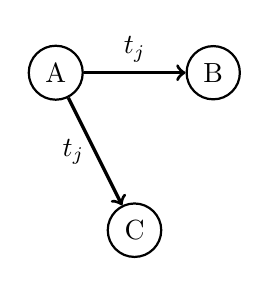
\begin{tikzpicture}
						\begin{scope}[every node/.style={circle,thick,draw}]
							\node (A) at (0,2) {A};
							\node (B) at (2,2) {B};
							\node (C) at (1,0) {C};
						\end{scope}
						
						\begin{scope}[every edge/.style={draw=black,very thick}]
							\path [->] (A) edge node [above] {$t_j$} (B);
							\path [->] (A) edge node [left] {$t_j$} (C);
						\end{scope}
					\end{tikzpicture}
					\caption{Event $(A,\{B,C\},t_j)$}
				\end{subfigure}
				\hfill
				\begin{subfigure}[t]{0.45\linewidth}
					\vskip 0pt
					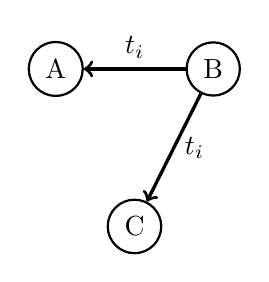
\begin{tikzpicture}
						\begin{scope}[every node/.style={circle,thick,draw}]
							\node (A) at (0,2) {A};
							\node (B) at (2,2) {B};
							\node (C) at (1,0) {C};
						\end{scope}
						
						\begin{scope}[every edge/.style={draw=black,very thick}]
							\path [->] (B) edge node [above] {$t_i$} (A);
							\path [->] (B) edge node [right] {$t_i$} (C);
						\end{scope}
					\end{tikzpicture}
					\caption{Event $(B,\{A,C\},t_i)$}
				\end{subfigure}
				\caption{Illustration of unordered repetition in relational hypereventevent models. Time ordering is $t_j < t_i$.}
				\label{fig:rhem_unordered_repetition}
			\end{mdframed}
		\end{figure}
	
		\item Partial repetition, i.e. the influence of the number of past events $e(h',<t_i)$ on the likelihood of a possible event $e(h,t_i)$, where $h' = (u,v'); \: h = (u,v); \: v \cap v' \neq \emptyset$ $\rightarrow$ is the likelihood of a future event $e(h,t_i)$ associated with the number of past events for which the target sets contain common actors? 
		\begin{align*}
			partial.repetition(e(h,t_i)) = \sum e(h',<t_i); \: h.source = h'.source \land h.targets \cap h'.targets \neq \emptyset
		\end{align*}
		\begin{figure}
			\begin{mdframed}
				\centering
				\begin{subfigure}[t]{0.45\linewidth}
					\vskip 0pt
					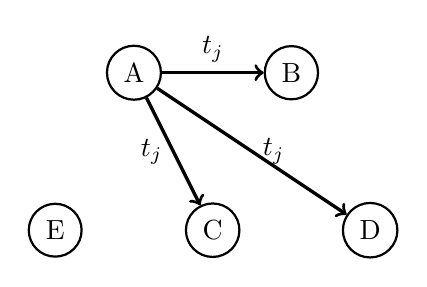
\begin{tikzpicture}
						\begin{scope}[every node/.style={circle,thick,draw}]
							\node (A) at (0,2) {A};
							\node (B) at (2,2) {B};
							\node (C) at (1,0) {C};
							\node (D) at (3,0) {D};
							\node (E) at (-1,0) {E};
						\end{scope}
						
						\begin{scope}[every edge/.style={draw=black,very thick}]
							\path [->] (A) edge node [above] {$t_j$} (B);
							\path [->] (A) edge node [left] {$t_j$} (C);
							\path [->] (A) edge node [right] {$t_j$} (D);
						\end{scope}
					\end{tikzpicture}
					\caption{Event $(A,\{B,C,D\},t_j)$}
				\end{subfigure}
				\hfill
				\begin{subfigure}[t]{0.45\linewidth}
					\vskip 0pt
					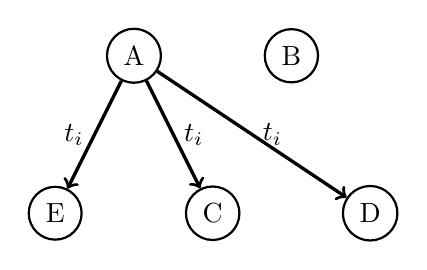
\begin{tikzpicture}
						\begin{scope}[every node/.style={circle,thick,draw}]
							\node (A) at (0,2) {A};
							\node (B) at (2,2) {B};
							\node (C) at (1,0) {C};
							\node (D) at (3,0) {D};
							\node (E) at (-1,0) {E};
						\end{scope}
						
						\begin{scope}[every edge/.style={draw=black,very thick}]
							\path [->] (A) edge node [right] {$t_i$} (C);
							\path [->] (A) edge node [right] {$t_i$} (D);
							\path [->] (A) edge node [left] {$t_i$} (E);
						\end{scope}
					\end{tikzpicture}
					\caption{Event $(A,\{C,D,E\},t_i)$}
				\end{subfigure}
				\caption{Illustration of partial repetition in relational hypereventevent models. Time ordering is $t_j < t_i$.}
				\label{fig:rhem_partial_repetition}
			\end{mdframed}
		\end{figure}
		
		\item Unordered partial repetition, i.e. the influence of past events $e(h',<t_i)$ on the likelihood of a possible event $e(h,t_i)$, where $h' \cap h \neq \emptyset$ $\rightarrow$ is the likelihood of a future event $e(h,t_i)$ associated with the number of past events on hyperedges which contain at least a subset of the same actors, but not necessarily in the same roles?
		\begin{align*}
			unordered.partial.repetition(e(h,t_i)) = \sum e(h',<t_i); \: h \cap h' \neq \emptyset
		\end{align*}
		\begin{figure}
			\begin{mdframed}
				\centering
				\begin{subfigure}[t]{0.45\linewidth}
					\vskip 0pt
					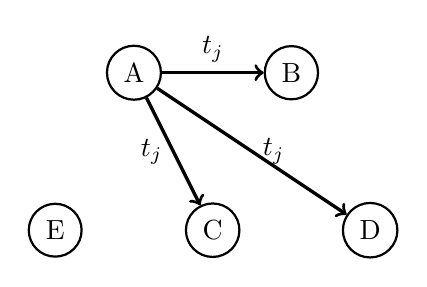
\begin{tikzpicture}
						\begin{scope}[every node/.style={circle,thick,draw}]
							\node (A) at (0,2) {A};
							\node (B) at (2,2) {B};
							\node (C) at (1,0) {C};
							\node (D) at (3,0) {D};
							\node (E) at (-1,0) {E};
						\end{scope}
						
						\begin{scope}[every edge/.style={draw=black,very thick}]
							\path [->] (A) edge node [above] {$t_j$} (B);
							\path [->] (A) edge node [left] {$t_j$} (C);
							\path [->] (A) edge node [right] {$t_j$} (D);
						\end{scope}
					\end{tikzpicture}
					\caption{Event $(A,\{B,C,D\},t_j)$}
				\end{subfigure}
				\hfill
				\begin{subfigure}[t]{0.45\linewidth}
					\vskip 0pt
					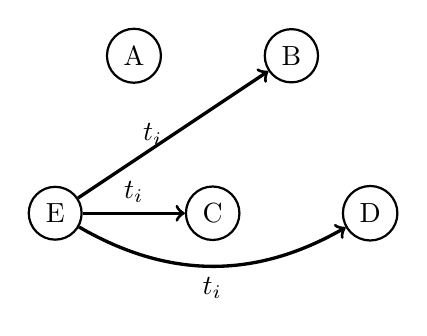
\begin{tikzpicture}
						\begin{scope}[every node/.style={circle,thick,draw}]
							\node (A) at (0,2) {A};
							\node (B) at (2,2) {B};
							\node (C) at (1,0) {C};
							\node (D) at (3,0) {D};
							\node (E) at (-1,0) {E};
						\end{scope}
						
						\begin{scope}[every edge/.style={draw=black,very thick}]
							\path [->] (E) edge node [left] {$t_i$} (B);
							\path [->] (E) edge node [above] {$t_i$} (C);
							\path [->] (E) edge [bend right] node [below] {$t_i$} (D);
						\end{scope}
					\end{tikzpicture}
					\caption{Event $(E,\{B,C,D\},t_i)$}
				\end{subfigure}
				\caption{Illustration of unordered partial repetition in relational hypereventevent models. Time ordering is $t_j < t_i$.}
				\label{fig:rhem_unordered_partial_repetition}
			\end{mdframed}
		\end{figure}
	
		\item Reciprocation, i.e. the influence of past events $e(h',<t_i)$ on the likelihood of a possible event $e(h,t_i)$, where $h' = (u',v'); \: h = (u,v); \: u \subset v' \land v \cap u' \neq \emptyset$ $\rightarrow$ is the likelihood of a future event $e(h,t_i)$ associated with the number of past events where the source of $e$ was part of the target set, and one of the targets of $e$ was the source?
		\begin{align*}
			reciprocation(e(h,t_i)) = \sum e(h',<t_i); \: h.source \subset h'.targets \land h'.source \subset h.targets
		\end{align*}
		\begin{figure}
			\begin{mdframed}
				\centering
				\begin{subfigure}[t]{0.45\linewidth}
					\vskip 0pt
					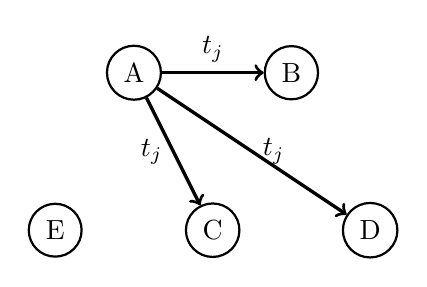
\begin{tikzpicture}
						\begin{scope}[every node/.style={circle,thick,draw}]
							\node (A) at (0,2) {A};
							\node (B) at (2,2) {B};
							\node (C) at (1,0) {C};
							\node (D) at (3,0) {D};
							\node (E) at (-1,0) {E};
						\end{scope}
						
						\begin{scope}[every edge/.style={draw=black,very thick}]
							\path [->] (A) edge node [above] {$t_j$} (B);
							\path [->] (A) edge node [left] {$t_j$} (C);
							\path [->] (A) edge node [right] {$t_j$} (D);
						\end{scope}
					\end{tikzpicture}
					\caption{Event $(A,\{B,C,D\},t_j)$}
				\end{subfigure}
				\hfill
				\begin{subfigure}[t]{0.45\linewidth}
					\vskip 0pt
					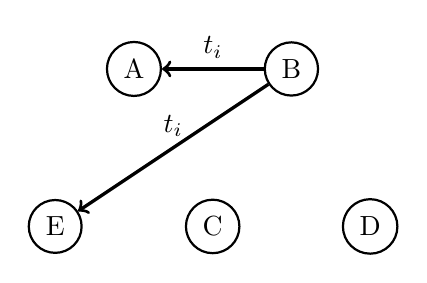
\begin{tikzpicture}
						\begin{scope}[every node/.style={circle,thick,draw}]
							\node (A) at (0,2) {A};
							\node (B) at (2,2) {B};
							\node (C) at (1,0) {C};
							\node (D) at (3,0) {D};
							\node (E) at (-1,0) {E};
						\end{scope}
						
						\begin{scope}[every edge/.style={draw=black,very thick}]
							\path [->] (B) edge node [above] {$t_i$} (A);
							\path [->] (B) edge node [above] {$t_i$} (E);
						\end{scope}
					\end{tikzpicture}
					\caption{Event $(B,\{A,E\},t_i)$}
				\end{subfigure}
				\caption{Illustration of reciprocation in relational hypereventevent models. Time ordering is $t_j < t_i$.}
				\label{fig:rhem_reciprocation}
			\end{mdframed}
		\end{figure}
	
		\item Nominator in-degree, i.e. the influence of past events $e(h',<t_i)$ on the likelihood of a possible event $e(h,t_i)$, where $h' = (u',v'); \: h = (u,v); \: u \subset v' \land v \cap v' = \emptyset$ $\rightarrow$ is the likelihood of a future event $e(h,t_i)$ associated with the number of past events where the source of $e$ was part of the target set, but none of the targets of $e$ was the source?
		\begin{align*}
			&nominator.indegree(e(h,t_i)) = \sum e(h',<t_i);&&\\
			&h.source \subset h'.targets \land h'.source \not\subset h.targets&&
		\end{align*}
		\begin{figure}
			\begin{mdframed}
				\centering
				\begin{subfigure}[t]{0.45\linewidth}
					\vskip 0pt
					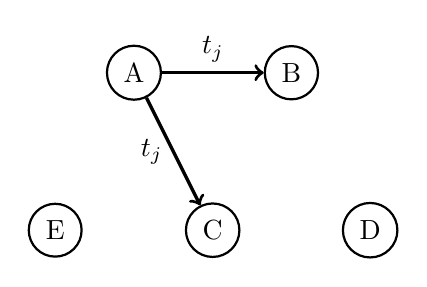
\begin{tikzpicture}
						\begin{scope}[every node/.style={circle,thick,draw}]
							\node (A) at (0,2) {A};
							\node (B) at (2,2) {B};
							\node (C) at (1,0) {C};
							\node (D) at (3,0) {D};
							\node (E) at (-1,0) {E};
						\end{scope}
						
						\begin{scope}[every edge/.style={draw=black,very thick}]
							\path [->] (A) edge node [above] {$t_j$} (B);
							\path [->] (A) edge node [left] {$t_j$} (C);
						\end{scope}
					\end{tikzpicture}
					\caption{Event $(A,\{B,C\},t_j)$}
				\end{subfigure}
				\hfill
				\begin{subfigure}[t]{0.45\linewidth}
					\vskip 0pt
					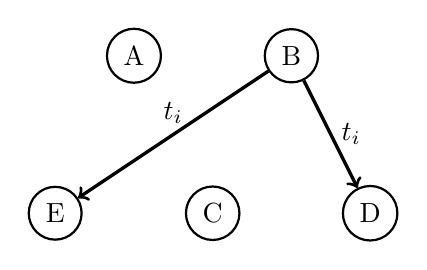
\begin{tikzpicture}
						\begin{scope}[every node/.style={circle,thick,draw}]
							\node (A) at (0,2) {A};
							\node (B) at (2,2) {B};
							\node (C) at (1,0) {C};
							\node (D) at (3,0) {D};
							\node (E) at (-1,0) {E};
						\end{scope}
						
						\begin{scope}[every edge/.style={draw=black,very thick}]
							\path [->] (B) edge node [right] {$t_i$} (D);
							\path [->] (B) edge node [above] {$t_i$} (E);
						\end{scope}
					\end{tikzpicture}
					\caption{Event $(B,\{D,E\},t_i)$}
				\end{subfigure}
				\caption{Illustration of nominator in-degree in relational hypereventevent models. Time ordering is $t_j < t_i$.}
				\label{fig:rhem_nominator_indegree}
			\end{mdframed}
		\end{figure}
	
		\item Nominee out-degree, i.e. the influence of past events $e(h',<t_i)$ on the likelihood of a possible event $e(h,t_i)$, where $h' = (u',v'); \: h = (u,v); \: u' \subset v \land u \not\in v'$ $\rightarrow$ is the likelihood of a future event $e(h,t_i)$ associated with the number of past events where one of the targets of $e$ was the source, but the source of $e$ was none of the targets?
		\begin{align*}
			&nominee.outdegree(e(h,t_i)) = \sum e(h',<t_i);&&\\
			&h'.source \subset h.targets \land h.source \not\subset h'.targets&&
		\end{align*}
		\begin{figure}
			\begin{mdframed}
				\centering
				\begin{subfigure}[t]{0.45\linewidth}
					\vskip 0pt
					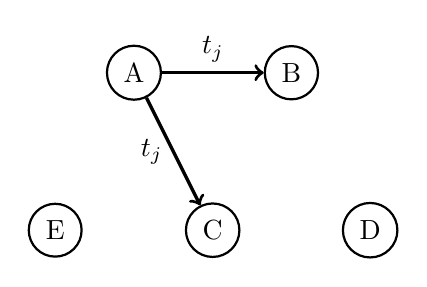
\begin{tikzpicture}
						\begin{scope}[every node/.style={circle,thick,draw}]
							\node (A) at (0,2) {A};
							\node (B) at (2,2) {B};
							\node (C) at (1,0) {C};
							\node (D) at (3,0) {D};
							\node (E) at (-1,0) {E};
						\end{scope}
						
						\begin{scope}[every edge/.style={draw=black,very thick}]
							\path [->] (A) edge node [above] {$t_j$} (B);
							\path [->] (A) edge node [left] {$t_j$} (C);
						\end{scope}
					\end{tikzpicture}
					\caption{Event $(A,\{B,C\},t_j)$}
				\end{subfigure}
				\hfill
				\begin{subfigure}[t]{0.45\linewidth}
					\vskip 0pt
					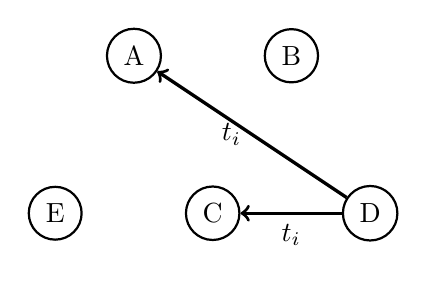
\begin{tikzpicture}
						\begin{scope}[every node/.style={circle,thick,draw}]
							\node (A) at (0,2) {A};
							\node (B) at (2,2) {B};
							\node (C) at (1,0) {C};
							\node (D) at (3,0) {D};
							\node (E) at (-1,0) {E};
						\end{scope}
						
						\begin{scope}[every edge/.style={draw=black,very thick}]
							\path [->] (D) edge node [left] {$t_i$} (A);
							\path [->] (D) edge node [below] {$t_i$} (C);
						\end{scope}
					\end{tikzpicture}
					\caption{Event $(D,\{A,C\},t_i)$}
				\end{subfigure}
				\caption{Illustration of nominee out-degree in relational hypereventevent models. Time ordering is $t_j < t_i$.}
				\label{fig:rhem_nominee_outdegree}
			\end{mdframed}
		\end{figure}
	
		\item Transitive tie, i.e. the influence of past events $e(h',t_j)$ and $e(\text{\emph{\^h}},t_k)$ on the likelihood of a possible event $e(h,t_i)$ ($t_j < t_k < t_i)$, where $h' = (u',v'); \: \text{\emph{\^h}} = (\text{\emph{\^u,\^v}}); \: h = (u,v); \: \text{\emph{\^u}} \subset v' \land v \cap v' \neq \emptyset$ $\rightarrow$ is there a tendency for triadic closure?
		\begin{align*}
			transitive.tie(e(h,t_i)) = \sum_{j \in h.targets} \sum_{a \in \mathcal{A}} \frac{min[d(h.source,\{a\}),d(a,\{j\})]}{\lvert h.targets \rvert}
		\end{align*}
		($\mathcal{A} \setminus \{h.source,j\}$ is the set of all actors $A$ excluding the source actor of $h$ and the iterated actor $j \in h.targets$, and $d(x,y)$ is the accumulated volume of interactions from $x$ to $y$ by the time $t_i$)
		\begin{figure}
			\begin{mdframed}
				\centering
				\begin{subfigure}[t]{0.3\linewidth}
					\vskip 0pt
					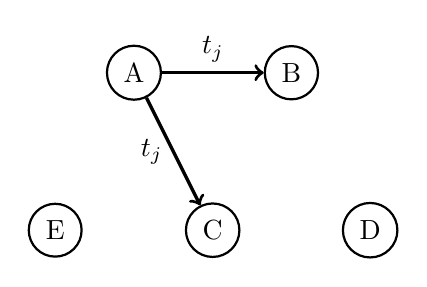
\begin{tikzpicture}
						\begin{scope}[every node/.style={circle,thick,draw}]
							\node (A) at (0,2) {A};
							\node (B) at (2,2) {B};
							\node (C) at (1,0) {C};
							\node (D) at (3,0) {D};
							\node (E) at (-1,0) {E};
						\end{scope}
						
						\begin{scope}[every edge/.style={draw=black,very thick}]
							\path [->] (A) edge node [above] {$t_j$} (B);
							\path [->] (A) edge node [left] {$t_j$} (C);
						\end{scope}
					\end{tikzpicture}
					\caption{Event $(A,\{B,C\},t_j)$}
				\end{subfigure}
				\hfill
				\begin{subfigure}[t]{0.3\linewidth}
					\vskip 0pt
					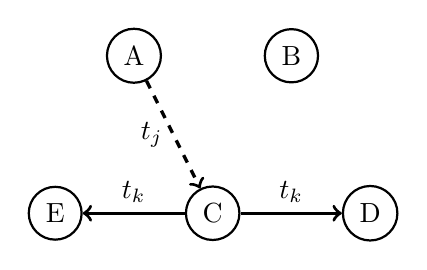
\begin{tikzpicture}
						\begin{scope}[every node/.style={circle,thick,draw}]
							\node (A) at (0,2) {A};
							\node (B) at (2,2) {B};
							\node (C) at (1,0) {C};
							\node (D) at (3,0) {D};
							\node (E) at (-1,0) {E};
						\end{scope}
						
						\begin{scope}[every edge/.style={draw=black,very thick}]
							\path [->] (A) edge [dashed] node [left] {$t_j$} (C);
							\path [->] (C) edge node [above] {$t_k$} (D);
							\path [->] (C) edge node [above] {$t_k$} (E);
						\end{scope}
					\end{tikzpicture}
					\caption{Event $(C,\{D,E\},t_i)$}
				\end{subfigure}
				\hfill
				\begin{subfigure}[t]{0.3\linewidth}
					\vskip 0pt
					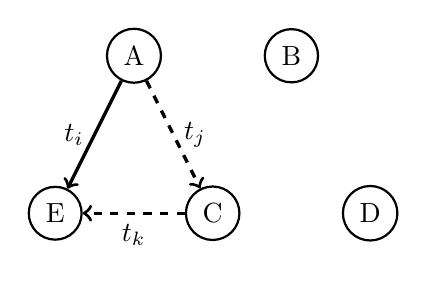
\begin{tikzpicture}
						\begin{scope}[every node/.style={circle,thick,draw}]
							\node (A) at (0,2) {A};
							\node (B) at (2,2) {B};
							\node (C) at (1,0) {C};
							\node (D) at (3,0) {D};
							\node (E) at (-1,0) {E};
						\end{scope}
						
						\begin{scope}[every edge/.style={draw=black,very thick}]
							\path [->] (A) edge [dashed] node [right] {$t_j$} (C);
							\path [->] (C) edge [dashed] node [below] {$t_k$} (E);
							\path [->] (A) edge node [left] {$t_i$} (E);
							%\path [->] (B) edge node [above] {$t_i$} (E);
						\end{scope}
					\end{tikzpicture}
					\caption{Event $(A,\{E\},t_i)$}
				\end{subfigure}
				\caption{Illustration of transitive tie in relational hypereventevent models. Time ordering is $t_j < t_k < t_i$. Dashed lines represent previous edges relevant to the closure.}
				\label{fig:rhem_transitive_tie}
			\end{mdframed}
		\end{figure}
	
		\item Cyclical tie, i.e. the influence of past events $e(h',t_j)$ and $e(\text{\emph{\^h}},t_k)$ on the likelihood of a possible event $e(h,t_i)$ ($t_j < t_k < t_i)$, where $h' = (u',v'); \: \text{\emph{\^h}} = (\text{\emph{\^u,\^v}}); \: h = (u,v); \: \text{\emph{\^u}} \subset v' \land u' \subset v$ $\rightarrow$ is there a tendency for cyclic closure?
		\begin{align*}
			cyclical.tie(e(h,t_i)) = \sum_{j \in h.targets} \sum_{a \in \mathcal{A}} \frac{min[d(a,\{h.source\}),d(j,\{a\})]}{\lvert h.targets \rvert}
		\end{align*}
		\begin{figure}
			\begin{mdframed}
				\centering
				\begin{subfigure}[t]{0.3\linewidth}
					\vskip 0pt
					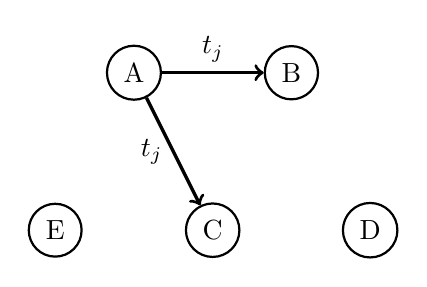
\begin{tikzpicture}
						\begin{scope}[every node/.style={circle,thick,draw}]
							\node (A) at (0,2) {A};
							\node (B) at (2,2) {B};
							\node (C) at (1,0) {C};
							\node (D) at (3,0) {D};
							\node (E) at (-1,0) {E};
						\end{scope}
						
						\begin{scope}[every edge/.style={draw=black,very thick}]
							\path [->] (A) edge node [above] {$t_j$} (B);
							\path [->] (A) edge node [left] {$t_j$} (C);
						\end{scope}
					\end{tikzpicture}
					\caption{Event $(A,\{B,C\},t_j)$}
				\end{subfigure}
				\hfill
				\begin{subfigure}[t]{0.3\linewidth}
					\vskip 0pt
					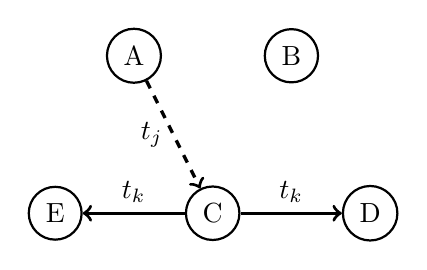
\begin{tikzpicture}
						\begin{scope}[every node/.style={circle,thick,draw}]
							\node (A) at (0,2) {A};
							\node (B) at (2,2) {B};
							\node (C) at (1,0) {C};
							\node (D) at (3,0) {D};
							\node (E) at (-1,0) {E};
						\end{scope}
						
						\begin{scope}[every edge/.style={draw=black,very thick}]
							\path [->] (A) edge [dashed] node [left] {$t_j$} (C);
							\path [->] (C) edge node [above] {$t_k$} (D);
							\path [->] (C) edge node [above] {$t_k$} (E);
						\end{scope}
					\end{tikzpicture}
					\caption{Event $(C,\{D,E\},t_i)$}
				\end{subfigure}
				\hfill
				\begin{subfigure}[t]{0.3\linewidth}
					\vskip 0pt
					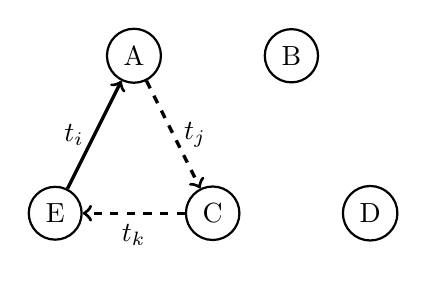
\begin{tikzpicture}
						\begin{scope}[every node/.style={circle,thick,draw}]
							\node (A) at (0,2) {A};
							\node (B) at (2,2) {B};
							\node (C) at (1,0) {C};
							\node (D) at (3,0) {D};
							\node (E) at (-1,0) {E};
						\end{scope}
						
						\begin{scope}[every edge/.style={draw=black,very thick}]
							\path [->] (A) edge [dashed] node [right] {$t_j$} (C);
							\path [->] (C) edge [dashed] node [below] {$t_k$} (E);
							\path [->] (E) edge node [left] {$t_i$} (A);
							%\path [->] (B) edge node [above] {$t_i$} (E);
						\end{scope}
					\end{tikzpicture}
					\caption{Event $(E,\{A\},t_i)$}
				\end{subfigure}
				\caption{Illustration of cyclical tie in relational hypereventevent models. Time ordering is $t_j < t_k < t_i$. Dashed lines represent previous edges relevant to the closure.}
				\label{fig:rhem_cyclical_tie}
				\end{mdframed}
			\end{figure}
		
			\item Shared source, i.e. the influence of past events $e(h',t_j)$ and $e(\text{\emph{\^h}},t_k)$ on the likelihood of a possible event $e(h,t_i)$ ($t_j < t_k < t_i)$, where $h' = (u',v'); \: \text{\emph{\^h}} = (\text{\emph{\^u,\^v}}); \: h = (u,v); \: u' = \text{\emph{\^u}} \land u \subset v' \land v \cap \text{\emph{\^v}} \neq \emptyset$ $\rightarrow$ are actors who were targets of the same source in previous events more likely to interact?
			\begin{align*}
				shared.source(e(h,t_i)) = \sum_{j \in h.targets} \sum_{a \in \mathcal{A}} \frac{min[d(a,\{h.source\}),d(a,\{j\})]}{\lvert h.targets \rvert}
			\end{align*}
			\begin{figure}
				\begin{mdframed}
					\centering
					\begin{subfigure}[t]{0.3\linewidth}
						\vskip 0pt
						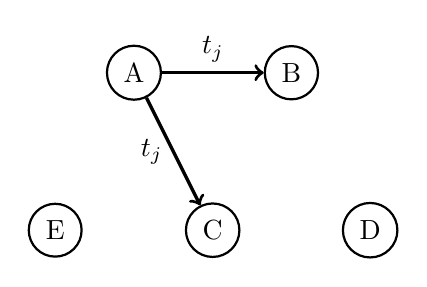
\begin{tikzpicture}
							\begin{scope}[every node/.style={circle,thick,draw}]
								\node (A) at (0,2) {A};
								\node (B) at (2,2) {B};
								\node (C) at (1,0) {C};
								\node (D) at (3,0) {D};
								\node (E) at (-1,0) {E};
							\end{scope}
							
							\begin{scope}[every edge/.style={draw=black,very thick}]
								\path [->] (A) edge node [above] {$t_j$} (B);
								\path [->] (A) edge node [left] {$t_j$} (C);
							\end{scope}
						\end{tikzpicture}
						\caption{Event $(A,\{B,C\},t_j)$}
					\end{subfigure}
					\hfill
					\begin{subfigure}[t]{0.3\linewidth}
						\vskip 0pt
						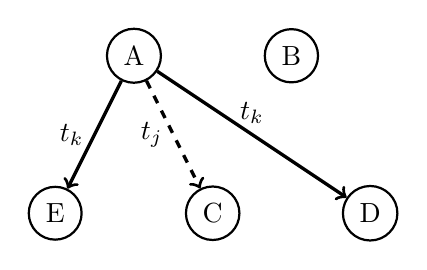
\begin{tikzpicture}
							\begin{scope}[every node/.style={circle,thick,draw}]
								\node (A) at (0,2) {A};
								\node (B) at (2,2) {B};
								\node (C) at (1,0) {C};
								\node (D) at (3,0) {D};
								\node (E) at (-1,0) {E};
							\end{scope}
							
							\begin{scope}[every edge/.style={draw=black,very thick}]
								\path [->] (A) edge [dashed] node [left] {$t_j$} (C);
								\path [->] (A) edge node [above] {$t_k$} (D);
								\path [->] (A) edge node [left] {$t_k$} (E);
							\end{scope}
						\end{tikzpicture}
						\caption{Event $(A,\{D,E\},t_i)$}
					\end{subfigure}
					\hfill
					\begin{subfigure}[t]{0.3\linewidth}
						\vskip 0pt
						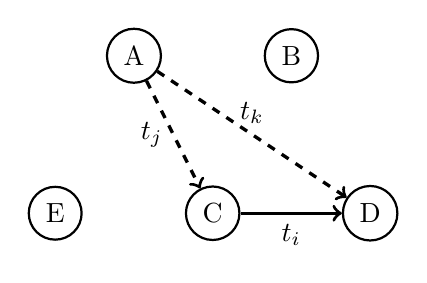
\begin{tikzpicture}
							\begin{scope}[every node/.style={circle,thick,draw}]
								\node (A) at (0,2) {A};
								\node (B) at (2,2) {B};
								\node (C) at (1,0) {C};
								\node (D) at (3,0) {D};
								\node (E) at (-1,0) {E};
							\end{scope}
							
							\begin{scope}[every edge/.style={draw=black,very thick}]
								\path [->] (A) edge [dashed] node [left] {$t_j$} (C);
								\path [->] (A) edge [dashed] node [above] {$t_k$} (D);
								\path [->] (C) edge node [below] {$t_i$} (D);
								%\path [->] (B) edge node [above] {$t_i$} (E);
							\end{scope}
						\end{tikzpicture}
						\caption{Event $(C,\{D\},t_i)$}
					\end{subfigure}
					\caption{Illustration of shared source in relational hypereventevent models. Time ordering is $t_j < t_k < t_i$. Dashed lines represent previous edges relevant to the closure.}
					\label{fig:rhem_shared_source}
				\end{mdframed}
		\end{figure}
	
		\item Shared target, i.e. the influence of past events $e(h',t_j)$ and $e(\text{\emph{\^h}},t_k)$ on the likelihood of a possible event $e(h,t_i)$ ($t_j < t_k < t_i)$, where $h' = (u',v'); \: \text{\emph{\^h}} = (\text{\emph{\^u,\^v}}); \: h = (u,v); \: v' \cap \text{\emph{\^v}} \neq \emptyset \land u = u' \land \text{\emph{\^u}} \subset v$ $\rightarrow$ are actors who targeted the same actors in previous events more likely to interact?
		\begin{align*}
			shared.target(e(h,t_i)) = \sum_{j \in h.targets} \sum_{a \in \mathcal{A}} \frac{min[d(h.source,\{a\}),d(j,\{a\})]}{\lvert h.targets \rvert}
		\end{align*}
		\begin{figure}
			\begin{mdframed}
				\centering
				\begin{subfigure}[t]{0.3\linewidth}
					\vskip 0pt
					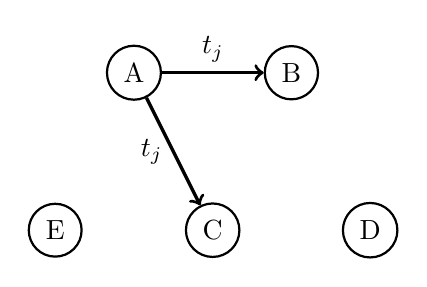
\begin{tikzpicture}
						\begin{scope}[every node/.style={circle,thick,draw}]
							\node (A) at (0,2) {A};
							\node (B) at (2,2) {B};
							\node (C) at (1,0) {C};
							\node (D) at (3,0) {D};
							\node (E) at (-1,0) {E};
						\end{scope}
						
						\begin{scope}[every edge/.style={draw=black,very thick}]
							\path [->] (A) edge node [above] {$t_j$} (B);
							\path [->] (A) edge node [left] {$t_j$} (C);
						\end{scope}
					\end{tikzpicture}
					\caption{Event $(A,\{B,C\},t_j)$}
				\end{subfigure}
				\hfill
				\begin{subfigure}[t]{0.3\linewidth}
					\vskip 0pt
					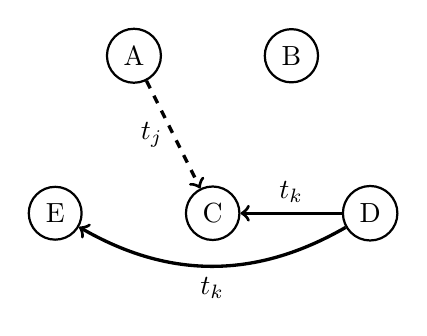
\begin{tikzpicture}
						\begin{scope}[every node/.style={circle,thick,draw}]
							\node (A) at (0,2) {A};
							\node (B) at (2,2) {B};
							\node (C) at (1,0) {C};
							\node (D) at (3,0) {D};
							\node (E) at (-1,0) {E};
						\end{scope}
						
						\begin{scope}[every edge/.style={draw=black,very thick}]
							\path [->] (A) edge [dashed] node [left] {$t_j$} (C);
							\path [->] (D) edge node [above] {$t_k$} (C);
							\path [->] (D) edge [bend left] node [below] {$t_k$} (E);
						\end{scope}
					\end{tikzpicture}
					\caption{Event $(D,\{C,E\},t_i)$}
				\end{subfigure}
				\hfill
				\begin{subfigure}[t]{0.3\linewidth}
					\vskip 0pt
					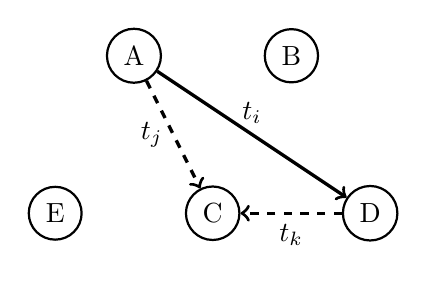
\begin{tikzpicture}
						\begin{scope}[every node/.style={circle,thick,draw}]
							\node (A) at (0,2) {A};
							\node (B) at (2,2) {B};
							\node (C) at (1,0) {C};
							\node (D) at (3,0) {D};
							\node (E) at (-1,0) {E};
						\end{scope}
						
						\begin{scope}[every edge/.style={draw=black,very thick}]
							\path [->] (A) edge [dashed] node [left] {$t_j$} (C);
							\path [->] (D) edge [dashed] node [below] {$t_k$} (C);
							\path [->] (A) edge node [above] {$t_i$} (D);
							%\path [->] (B) edge node [above] {$t_i$} (E);
						\end{scope}
					\end{tikzpicture}
					\caption{Event $(A,\{D\},t_i)$}
				\end{subfigure}
				\caption{Illustration of shared target in relational hypereventevent models. Time ordering is $t_j < t_k < t_i$. Dashed lines represent previous edges relevant to the closure.}
				\label{fig:rhem_shared_target}
			\end{mdframed}
		\end{figure}
	
	\end{itemize}
	\item Effects depending on actor attributes:
	\begin{itemize}
		\item Nominator age
		\item Nominees average age
		\item Nominator-nominees age difference
		\item Nominees age difference
		\item Nominator sex
		\item Nominees average sex
		\item Nominator-nominees sex difference
		\item Nominees sex difference
		\item Other covariates specific to the individual datasets, which are listed in section \ref{ch:previous_work_data}. In general, there are four statistics for each covariate: the value of the nominator, the average value of the nominees, the difference in value between nominator and nominees, and the difference in value between nominees.
	\end{itemize}
\end{itemize}

\noindent These statistics were likewise calculated using the \emph{eventnet} software \cite{eventnet_rem,eventnet_rhem}. Using the \emph{R} package \emph{survival} \cite{survival-package}, a Cox proportional hazards model was fitted on the result tables in order to estimate the model parameters $\theta$, and therefore draw conclusions regarding significance and effect of the individual statistics. Results are presented and discussed in chapter \ref{ch:results_discussion}.


	\chapter{4\quad Results and Discussion}
\label{ch:results_discussion}

\section{Results of Social Network Analysis across regions}
\label{sec:res_sna}

\subsection{One-way ANOVAs for network statistics}
\label{sec:sna_anovas}

One of the goals of this work is to investigate whether there are significant differences between the different datasets in terms of network statistics. This knowledge might be used e.g. to the impact of different containment methods. One-way ANOVAs with multiple comparisons were used to identify significant differences between the networks derived from the datasets. Furthermore, descriptive statistics are given for all computed network statistics.

\paragraph{Degree centrality} Recall that degree centrality values are normalised; therefore comparison values derived from original publications are adjusted accordingly. Average values for the different regions were $0.0071\pm0.016$ for the Yunnan dataset ($1.345\pm3.187$ reported in the original publication \cite{hainan_publication}; $0.0079\pm0.018$ adjusted for normalisation), $0.0093\pm0.011$ for the Hainan dataset ($1.51\pm1.79$ reported in the original publication \cite{hainan_publication}; $0.0093\pm0.011$ adjusted for normalisation), $0.0043\pm0.0056$ for the Shaanxi dataset ($0.987\pm1.351$ reported in the original publication \cite{shaanxi_publication}; $0.0041\pm0.0057$ adjusted for normalisation), $0.00036\pm0.00067$ for the Xi'an dataset ($0.741\pm1.379$ in the original publication \cite{xian_publication}; $0.00036\pm0.00067$ adjusted for normalisation), $1.80\cdot 10^{-5}\pm6.84\cdot 10^{-5}$ for the China dataset (no data reported in the original publication), and $7.9\cdot 10^{-6}\pm1.4\cdot 10^{-5}$ for the Bucharest dataset (no data reported in the original publication). Therefore, values could reliably be reproduced where applicable, assuming some loss of precision.

\begin{table}[htbp]
	\begin{mdframed}
		\begin{tabular*}{\linewidth}{l|llllll}
			\hline
			\textbf{ } & \textbf{Yunnan} & \textbf{Hainan} & \textbf{Shaanxi} & \textbf{Xi'an} & \textbf{Bucharest} & \textbf{China}\\
			\hline
			\textbf{N} & 171 & 162 & 237 & 2050 & 57836 & 25877\\
			\textbf{Minimum} & 0.0 & 0.0 & 0.0 & 0.0 & 0.0 & 0.0\\
			\textbf{25 Percentile} & 0.0 & 0.0 & 0.0 & 0.0 & 0.0 & 0.0\\
			\textbf{Median} & 0.0 & 0.0062 & 0.0042 & 0.00048 & 0.0 & 0.0\\
			\textbf{75 Percentile} & 0.0058 & 0.018 & 0.0084 & 0.00048 & $1.72\cdot 10^{-5}$ & 0.0\\
			\textbf{Maximum} & 0.070 & 0.037 & 0.046 & 0.020 & 0.00032 & 0.0052\\
			\textbf{Mean} & 0.0071 & 0.0093 & 0.0043 & 0.00036 & $7.93\cdot 10^{-6}$ & $1.80\cdot 10^{-5}$\\
			\textbf{Std. Dev.} & 0.016 & 0.011 & 0.0056 & 0.00067 & $1.42\cdot 10^{-5}$ & $6.74\cdot 10^{-5}$\\
			\hline
		\end{tabular*}
		\caption{Descriptive statistics for degree centrality.}
		\label{tab:degree_centrality_desc}
		\vskip 10pt
		\small
		\begin{tabular*}{\linewidth}{l|llll}
			\hline
			\textbf{Pair} & \textbf{Mean Diff.} & \textbf{95\% CI of diff.} & \textbf{Sign.?} & \textbf{Adj. P value}\\
			\hline
			Yunnan vs. Hainan & -0.0022 & -0.0024 to -0.0019 & Yes & $<0.0001$\\
			Yunnan vs. Shaanxi & 0.0028 & 0.0025 to 0.0030 & Yes & $<0.0001$\\
			Yunnan vs. Bucharest & 0.0071 & 0.0069 to 0.0073 & Yes & $<0.0001$\\
			Yunnan vs. China & 0.0071 & 0.0069 to 0.0073 & Yes & $<0.0001$\\
			Yunnan vs. Xi'an & 0.0067 & 0.0065 to 0.0070 & Yes & $<0.0001$\\
			Hainan vs. Shaanxi & 0.0050 & 0.0047 to 0.0053 & Yes & $<0.0001$\\
			Hainan vs. Bucharest & 0.0093 & 0.0091 to 0.0095 & Yes & $<0.0001$\\
			Hainan vs. China & 0.0093 & 0.0091 to 0.0095 & Yes & $<0.0001$\\
			Hainan vs. Xi'an & 0.0089 & 0.0087 to 0.0092 & Yes & $<0.0001$\\
			Shaanxi vs. Bucharest & 0.0043 & 0.0041 to 0.0044 & Yes & $<0.0001$\\
			Shaanxi vs. China & 0.0043 & 0.0041 to 0.0044 & Yes & $<0.0001$\\
			Shaanxi vs. Xi'an & 0.0039 & 0.0037 to 0.0041 & Yes & $<0.0001$\\
			Bucharest vs. China & $-1.01\cdot 10^{-5}$ & $-3.00\cdot 10^{-5}$ to $9.76\cdot 10^{-6}$ & No & 0.6956\\
			Bucharest vs. Xi'an & -0.00035 & -0.00041 to -0.00029 & Yes & $<0.0001$\\
			China vs. Xi'an & -0.00034 & -0.00040 to -0.00028 & Yes & $<0.0001$\\
			\hline
		\end{tabular*}
		\caption{Multiple comparisons for degree centrality. Method is Tukey's multiple comparison test with an alpha value of 0.05 (i.e. 95\% confidence interval).}
		\label{tab:degree_centrality_tukey}
	\end{mdframed}
\end{table}

One-way ANOVA comparison between the regions found a significant difference between the means ($F(5,86327) = 6265; \: p<0.0001$). Compared against each other (using Tukey's multiple comparisons test with 95\% confidence interval), all regions were pairwise significantly different except Bucharest vs. China ($p=0.6956$).

\paragraph{Betweenness centrality} Average values for the different regions were $7.32\cdot 10^{-6}\pm3.67\cdot 10^{-5}$ for the Yunnan dataset ($0.0000\pm0.0000$ reported in the original publication \cite{hainan_publication}), $1.72\cdot 10^{-5}\pm1.09\cdot 10^{-4}$ for the Hainan dataset ($0.0000\pm0.0001$ reported in the original publication \cite{hainan_publication}), $1.68\cdot 10^{-5}\pm1.02\cdot 10^{-4}$ for the Shaanxi dataset ($0.0000\pm0.0001$ reported in the original publication \cite{shaanxi_publication}), $1.60\cdot 10^{-6}\pm2.41\cdot 10^{-5}$ for the Xi'an dataset (no data reported in the original publication), $5.18\cdot 10^{-5}\pm0.01$ for the Bucharest dataset (no data reported in the original publication), and $2.33\cdot 10^{-8}\pm9.05\cdot 10^{-7}$ for the China dataset (no data reported in the original publication). Taking into account that values only include four digits after the decimal point and the resulting loss of information, values could reliably be reproduced where applicable.

\begin{table}[htbp]
	\begin{mdframed}
		\begin{tabular*}{\linewidth}{l|llllll}
			\hline
			\textbf{ } & \textbf{Yunnan} & \textbf{Hainan} & \textbf{Shaanxi} & \textbf{Xi'an} & \textbf{Bucharest} & \textbf{China}\\
			\hline
			\textbf{N} & 171 & 162 & 237 & 2050 & 57836 & 25877\\
			\textbf{Minimum} & 0.0 & 0.0 & 0.0 & 0.0 & 0.0 & 0.0\\
			\textbf{25 Percentile} & 0.0 & 0.0 & 0.0 & 0.0 & 0.0 & 0.0\\
			\textbf{Median} & 0.0 & 0.0 & 0.0 & 0.0 & 0.0 & 0.0\\
			\textbf{75 Percentile} & 0.0 & 0.0 & 0.0 & 0.0 & 0.0 & 0.0\\
			\textbf{Maximum} & 0.00034 & 0.0012 & 0.0013 & 0.00079 & 3.0 & $9.40\cdot 10^{-5}$\\
			\textbf{Mean} & $7.32\cdot 10^{-6}$ & $1.72\cdot 10^{-5}$ & $1.68\cdot 10^{-5}$ & $1.60\cdot 10^{-6}$ & $5.18\cdot 10^{-5}$ & $2.33\cdot 10^{-8}$\\
			\textbf{Std. Dev.} & $3.67\cdot 10^{-5}$ & 0.00010 & 0.00010 & $2.41\cdot 10^{-5}$ & 0.012 & $9.05\cdot 10^{-7}$\\
			\hline
		\end{tabular*}
		\caption{Descriptive statistics for betweenness centrality.}
		\label{tab:betweenness_centrality_desc}
		\vskip 10pt
		\small
		\begin{tabular*}{\linewidth}{l|llll}
			\hline
			\textbf{Pair} & \textbf{Mean Diff.} & \textbf{95\% CI of diff.} & \textbf{Sign.?} & \textbf{Adj. P value}\\
			\hline
			Yunnan vs. Hainan & $-9.92\cdot 10^{-6}$ & -0.0032 to 0.0031 & No & $>0.9999$\\
			Yunnan vs. Shaanxi & $-9.56\cdot 10^{-6}$ & -0.0029 to 0.0029 & No & $>0.9999$\\
			Yunnan vs. Bucharest & $-4.45\cdot 10^{-5}$ & -0.0022 to 0.0021 & No & $>0.9999$\\
			Yunnan vs. China & $7.30\cdot 10^{-6}$ & -0.0022 to 0.0022 & No & $>0.9999$\\
			Yunnan vs. Xi'an & $5.72\cdot 10^{-6}$ & -0.0023 to 0.0023 & No & $>0.9999$\\
			Hainan vs. Shaanxi & $3.63\cdot 10^{-7}$ & -0.0029 to 0.0029 & No & $>0.9999$\\
			Hainan vs. Bucharest & $-3.46\cdot 10^{-5}$ & -0.0023 to 0.0022 & No & $>0.9999$\\
			Hainan vs. China & $1.72\cdot 10^{-5}$ & -0.0022 to 0.0023 & No & $>0.9999$\\
			Hainan vs. Xi'an & $1.56\cdot 10^{-5}$ & 0.0023 to 0.0023 & No & $>0.9999$\\
			Shaanxi vs. Bucharest & $-3.49\cdot 10^{-5}$ & -0.0019 to 0.0018 & No & $>0.9999$\\
			Shaanxi vs. China & $1.68\cdot 10^{-5}$ & -0.0018 to 0.0019 & No & $>0.9999$\\
			Shaanxi vs. Xi'an & $1.52\cdot 10^{-5}$ & -0.0019 to 0.0020 & No & $>0.9999$\\
			Bucharest vs. China & $5.18\cdot 10^{-5}$ & -0.00016 to 0.00026 & No & 0.9843\\
			Bucharest vs. Xi'an & $5.02\cdot 10^{-5}$ & -0.00060 to 0.00070 & No & $>0.9999$\\
			China vs. Xi'an & $-1.58\cdot 10^{-6}$ & -0.00066 to 0.00066 & No & $>0.9999$\\
			\hline
		\end{tabular*}
		\caption{Multiple comparisons for betweenness centrality. Method is Tukey's multiple comparison test with an alpha value of 0.05 (i.e. 95\% confidence interval).}
		\label{tab:betweenness_centrality_tukey}
	\end{mdframed}
\end{table}

One-way ANOVA comparison between the regions found no significant difference between the means $F(5,86327) = 0.09719; \: p=0.9926$). Compared against each other (Tukey's test, 95\% CI), no regions were pairwise significantly different.

\paragraph{Pagerank centrality} Average values for the different regions were $0.0058\pm0.0055$ for the Yunnan dataset ($0.0058\pm0.0055$ reported in the original publication \cite{hainan_publication}), $0.0061\pm0.0043$ for the Hainan dataset ($0.0062\pm0.0043$ reported in the original publication \cite{hainan_publication}), $0.0042\pm0.0034$ for the Shaanxi dataset ($0.0042\pm0.0035$ reported in the original publication \cite{shaanxi_publication}), $0.00048\pm0.00057$ for the Xi'an dataset ($0.0005\pm0.0006$ reported in the original publication \cite{xian_publication}), $6.91\cdot 10^{-5}\pm0.01$ for the Bucharest dataset (no data reported in the original publication), and $3.86\cdot 10^{-5}\pm6.07\cdot 10^{-5}$ for the China dataset (no data reported in the original publication). Therefore, values could reliably be reproduced where applicable, assuming some loss of precision.

\begin{table}[htbp]
	\begin{mdframed}
		\begin{tabular*}{\linewidth}{l|llllll}
			\hline
			\textbf{ } & \textbf{Yunnan} & \textbf{Hainan} & \textbf{Shaanxi} & \textbf{Xi'an} & \textbf{Bucharest} & \textbf{China}\\
			\hline
			\textbf{N} & 171 & 162 & 237 & 2050 & 57836 & 25877\\
			\textbf{Minimum} & 0.0020 & 0.0014 & 0.00099 & 0.00012 & $6.09\cdot 10^{-6}$ & $1.87\cdot 10^{-5}$\\
			\textbf{25 Percentile} & 0.0020 & 0.0014 & 0.00099 & 0.00012 & $6.09\cdot 10^{-6}$ & $1.87\cdot 10^{-5}$\\
			\textbf{Median} & 0.0020 & 0.0081 & 0.0043 & 0.00044 & $6.09\cdot 10^{-6}$ & $1.87\cdot 10^{-5}$\\
			\textbf{75 Percentile} & 0.013 & 0.0098 & 0.0066 & 0.00081 & $2.60\cdot 10^{-5}$ & $1.87\cdot 10^{-5}$\\
			\textbf{Maximum} & 0.022 & 0.018 & 0.023 & 0.016 & 3.0 & 0.0047\\
			\textbf{Mean} & 0.0058 & 0.0061 & 0.0042 & 0.00048 & $6.91\cdot 10^{-5}$ & $3.86\cdot 10^{-5}$\\
			\textbf{Std. Dev.} & 0.0055 & 0.0043 & 0.0034 & 0.00057 & 0.012 & $6.07\cdot 10^{-5}$\\
			\hline
		\end{tabular*}
		\caption{Descriptive statistics for pagerank centrality.}
		\label{tab:pagerank_centrality_desc}
		\vskip 10pt
		\small
		\begin{tabular*}{\linewidth}{l|llll}
			\hline
			\textbf{Pair} & \textbf{Mean Diff.} & \textbf{95\% CI of diff.} & \textbf{Sign.?} & \textbf{Adj. P value}\\
			\hline
			Yunnan vs. Hainan & -0.00032 & -0.0035 to 0.0028 & No & 0.9997\\
			Yunnan vs. Shaanxi & 0.0016 & -0.0012 to 0.0045 & No & 0.6061\\
			Yunnan vs. Bucharest & 0.0057 & 0.0035 to 0.0080 & Yes & $<0.0001$\\
			Yunnan vs. China & 0.0058 & 0.0035 to 0.0080 & Yes & $<0.0001$\\
			Yunnan vs. Xi'an & 0.0053 & 0.0030 to 0.0076 & Yes & $<0.0001$\\
			Hainan vs. Shaanxi & 0.0019 & -0.0010 to 0.0049 & No & 0.4173\\
			Hainan vs. Bucharest & 0.0061 & 0.0038 to 0.0083 & Yes & $<0.0001$\\
			Hainan vs. China & 0.0061 & 0.0038 to 0.0084 & Yes & $<0.0001$\\
			Hainan vs. Xi'an & 0.0056 & 0.0033 to 0.0080 & Yes & $<0.0001$\\
			Shaanxi vs. Bucharest & 0.0041 & 0.0022 to 0.0060 & Yes & $<0.0001$\\
			Shaanxi vs. China & 0.0041 & 0.0022 to 0.0060 & Yes & $<0.0001$\\
			Shaanxi vs. Xi'an & 0.0037 &0.0017 to 0.0057 & Yes & $<0.0001$\\
			Bucharest vs. China & $3.05\cdot 10^{-5}$ & -0.00018 to 0.00024 & No & 0.9987\\
			Bucharest vs. Xi'an & -0.00041 & -0.0010 to 0.00023 & No & 0.4507\\
			China vs. Xi'an & -0.00044 & -0.0011 to 0.00021 & No & 0.3922\\
			\hline
		\end{tabular*}
		\caption{Multiple comparisons for pagerank centrality. Method is Tukey's multiple comparison test with an alpha value of 0.05 (i.e. 95\% confidence interval).}
		\label{tab:pagerank_centrality_tukey}
	\end{mdframed}
\end{table}

One-way ANOVA comparison between the regions found a significant difference between the means ($F(5,86327) = 38.86; \: p<0.0001$). Compared against each other (Tukey's test, 95\% CI), results were mixed. There was no significant difference for Yunnan vs. Hainan ($p=0.9997$), Yunnan vs. Shaanxi ($p=0.6061$), Hainan vs. Shaanxi ($p=0.4173$), Bucharest vs. China ($p=0.9987$), Bucharest vs. Xi'an ($p=0.4507$), and China vs. Xi'an ($p=0.3922$). All other pairs were significantly different.

\paragraph{Component size} Average values for the different regions were $2.42\pm3.23$ for the Yunnan dataset, $2.85\pm2.32$ for the Hainan dataset, $2.86\pm2.71$ for the Shaanxi dataset, $5.23\pm12.34$ for the Xi'an dataset, $1.93\pm1.79$ for the Bucharest dataset, and $6.76\pm38.15$ for the China dataset. No values were reported in the original publications, only individual clusters were examined in an exploratory fashion in \cite{hainan_publication,shaanxi_publication,xian_publication}.

\begin{table}[htbp]
	\begin{mdframed}
		\begin{tabular*}{\linewidth}{l|llllll}
			\hline
			\textbf{ } & \textbf{Yunnan} & \textbf{Hainan} & \textbf{Shaanxi} & \textbf{Xi'an} & \textbf{Bucharest} & \textbf{China}\\
			\hline
			\textbf{N} & 171 & 162 & 237 & 2050 & 57836 & 25877\\
			\textbf{Minimum} & 1.0 & 1.0 & 1.0 & 1.0 & 1.0 & 1.0\\
			\textbf{25 Percentile} & 1.0 & 1.0 & 1.0 & 1.0 & 1.0 & 1.0\\
			\textbf{Median} & 1.0 & 2.0 & 2.0 & 2.0 & 1.0 & 1.0\\
			\textbf{75 Percentile} & 2.0 & 4.0 & 4.0 & 4.0 & 2.0 & 1.0\\
			\textbf{Maximum} & 13.0 & 9.0 & 12.0 & 64.0 & 20.0 & 329.0\\
			\textbf{Mean} & 2.42 & 2.85 & 2.86 & 5.23 & 1.93 & 6.76\\
			\textbf{Std. Dev.} & 3.23 & 2.32 & 2.71 & 12.34 & 1.79 & 38.15\\
			\hline
		\end{tabular*}
		\caption{Descriptive statistics for component size.}
		\label{tab:component_size_desc}
		\vskip 10pt
		\small
		\begin{tabular*}{\linewidth}{l|llll}
			\hline
			\textbf{Pair} & \textbf{Mean Diff.} & \textbf{95\% CI of diff.} & \textbf{Sign.?} & \textbf{Adj. P value}\\
			\hline
			Yunnan vs. Hainan & -0.42 & -6.99 to 6.14 & No & $>0.9999$\\
			Yunnan vs. Shaanxi & -0.43 & -6.45 to 5.57 & No & $>0.9999$\\
			Yunnan vs. Bucharest & 0.49 & -4.09 to 5.08 & No & 0.9996\\
			Yunnan vs. China & -4.33 & -8.93 to 0.25 & No & 0.0772\\
			Yunnan vs. Xi'an & -2.81 & -7.58 to 1.95 & No & 0.5452\\
			Hainan vs. Shaanxi & -0.013 & -6.12 to 6.09 & No & $>0.9999$\\
			Hainan vs. Bucharest & 0.92 & -3.79 to 5.63 & No & 0.9936\\
			Hainan vs. China & -3.91 & -8.63 to 0.80 & No & 0.1698\\
			Hainan vs. Xi'an & -2.38 & -7.27 to 2.50 & No & 0.7328\\
			Shaanxi vs. Bucharest & 0.93 & -2.96 to 4.83 & No & 0.9838\\
			Shaanxi vs. China & -3.90 & -7.81 to 0.0087 & No & 0.0509\\
			Shaanxi vs. Xi'an & -2.37 & -6.48 to 1.73 & No & 0.5684\\
			Bucharest vs. China & -4.83 & -5.28 to -4.38 & Yes & $<0.0001$\\
			Bucharest vs. Xi'an & -3.30 & -4.65 to -1.96 & Yes & $<0.0001$\\
			China vs. Xi'an & 1.52 & 0.15 to 2.90 & Yes & 0.0192\\
			\hline
		\end{tabular*}
		\caption{Multiple comparisons for component sizes. Method is Tukey's multiple comparison test with an alpha value of 0.05 (i.e. 95\% confidence interval).}
		\label{tab:component_size_tukey}
	\end{mdframed}
\end{table}

One-way ANOVA comparison between the regions found a significant difference between the means ($F(5,86326) = 192.3; \: p<0.0001$). Compared against each other (Tukey's test, 95\% CI), no pairs were significantly different from each other except Bucharest vs. China, Bucharest vs. Xi'an, and China vs. Xi'an.

\paragraph{Average shortest path length} Average values for the different regions were $0.25\pm0.39$ for the Yunnan dataset, $0.45\pm0.47$ for the Hainan dataset, $0.52\pm0.56$ for the Shaanxi dataset, $0.61\pm0.80$ for the Xi'an dataset, $0.32\pm0.51$ for the Bucharest dataset, and $0.24\pm0.67$ for the China dataset. Shortest path length was not analysed in any of the previous works, therefore there are no comparison values.

\begin{table}[htbp]
	\begin{mdframed}
		\begin{tabular*}{\linewidth}{l|llllll}
			\hline
			\textbf{ } & \textbf{Yunnan} & \textbf{Hainan} & \textbf{Shaanxi} & \textbf{Xi'an} & \textbf{Bucharest} & \textbf{China}\\
			\hline
			\textbf{N} & 171 & 162 & 237 & 2050 & 57836 & 25877\\
			\textbf{Minimum} & 0.0 & 0.0 & 0.0 & 0.0 & 0.0 & 0.0\\
			\textbf{25 Percentile} & 0.0 & 0.0 & 0.0 & 0.0 & 0.0 & 0.0\\
			\textbf{Median} & 0.0 & 0.5 & 0.5 & 0.5 & 0.0 & 0.0\\
			\textbf{75 Percentile} & 0.5 & 0.75 & 1.0 & 1.0 & 0.5 & 0.0\\
			\textbf{Maximum} & 1.53 & 1.88 & 2.0 & 4.62 & 4.25 & 7.24\\
			\textbf{Mean} & 0.25 & 0.45 & 0.52 & 0.61 & 0.32 & 0.24\\
			\textbf{Std. Dev.} & 0.39 & 0.47 & 0.56 & 0.80 & 0.51 & 0.67\\
			\hline
		\end{tabular*}
		\caption{Descriptive statistics for average shortest path length per vertex.}
		\label{tab:avg_shortest_path_desc}
		\vskip 10pt
		\small
		\begin{tabular*}{\linewidth}{l|llll}
			\hline
			\textbf{Pair} & \textbf{Mean Diff.} & \textbf{95\% CI of diff.} & \textbf{Sign.?} & \textbf{Adj. P value}\\
			\hline
			Yunnan vs. Hainan & -0.20 & -0.38 to -0.023 & Yes & 0.0164\\
			Yunnan vs. Shaanxi & -0.26 & -0.43 to -0.10 & Yes & $<0.0001$\\
			Yunnan vs. Bucharest & -0.070 & -0.19 to 0.055 & No & 0.5994\\
			Yunnan vs. China & 0.0093 & -0.11 to 0.13 & No & $>0.9999$\\
			Yunnan vs. Xi'an & -0.35 & -0.48 to -0.22 & Yes & $<0.0001$\\
			Hainan vs. Shaanxi & -0.066 & -0.23 to 0.10 & No & 0.8659\\
			Hainan vs. Bucharest & 0.13 & 0.0034 to 0.26 & Yes & 0.0401\\
			Hainan vs. China & 0.21 & 0.083 to 0.34 & Yes & $<0.0001$\\
			Hainan vs. Xi'an & -0.15 & -0.29 to -0.022 & Yes & 0.0111\\
			Shaanxi vs. Bucharest & 0.19 & 0.092 to 0.30 & Yes & $<0.0001$\\
			Shaanxi vs. China & 0.27 & 0.17 to 0.38 & Yes & $<0.0001$\\
			Shaanxi vs. Xi'an & -0.089 & -0.20 to 0.022 & No & 0.2042\\
			Bucharest vs. China & 0.079 & 0.067 to 0.092 & Yes & $<0.0001$\\
			Bucharest vs. Xi'an & -0.28 & -0.32 to -0.25 & Yes & $<0.0001$\\
			China vs. Xi'an & -0.36 & -0.40 to -0.33 & Yes & $<0.0001$\\
			\hline
		\end{tabular*}
		\caption{Multiple comparisons for average shortest path length per vertex. Method is Tukey's multiple comparison test with an alpha value of 0.05 (i.e. 95\% confidence interval).}
		\label{tab:avg_shortest_path_tukey}
	\end{mdframed}
\end{table}

One-way ANOVA comparison between the regions found a significant difference between the means ($F(5,86326)=196.8; \: p<0.0001$). Compared against each other (Tukey's test, 95\% CI), results were mixed. There was no significant difference for Yunnan vs. Bucharest ($p=0.5994$), Yunnan vs. China ($p>0.9999$), Hainan vs. Shaanxi ($p=0.8659$), and Shaanxi vs Xi'an ($p=0.2042$). All other pairs were significantly different.

\subsection{Regression models for contact nomination likelihood}
\label{sec:sna_regression}

As briefly stated in chapter \ref{ch:methods}, ordinary least-squares regression was subsequently used to determine the influence of network statistics and actor covariates on contact nomination likelihood. To this end, for each dataset, all possible actor combinations were compiled into a dataset; each record contains network statistics and actor covariates of the source and target, and the absolute difference between source and target values for each variable. The regression model is fitted on the complete dataset, conditioned on whether there is a contact nomination seen in the actual underlying data (i.e. the original data presented in chapter \ref{ch:previous_work_data}). Therefore, the focus lies on explaining rather than predicting contact nominations. As covariates differ between the datasets, a different model was created for each dataset. The Xi'an dataset was excluded from this analysis, as it unfortunately does not include patient covariates.

\paragraph{Yunnan network} With a 95\% confidence interval, the statistically significant predictors for contact nomination likelihood are the sex of the nominator ($p<0.001$), sex discrepancy between nominator and nominee ($p<0.001$), whether the nominator is a family member of another actor in the dataset ($p<0.001$), and all network statistics for nominator, nominee, and the difference between nominator and nominee, with the exception of the average shortest path length of the nominator ($p=0.224$). Nominator sex has a marginally positive effect on contact nomination likelihood (coefficient = 0.0036); sex discrepancy has a marginally positive effect (coefficient = 0.0033); family member status of the nominator has a marginally positive effect (coefficient = 0.0036); degree centrality of nominator and nominee both have a slightly positive effect (coefficients = 0.0874 and 0.0901), while degree centrality discrepancy has a slightly negative effect (coefficient = -0.0880); betweenness centrality of nominator and nominee both have a slightly negative effect (covariates = -0.0103 and -0.0114), while betweenness centrality discrepancy has a slightly positive effect (coefficient = 0.0182); pagerank centrality of the nominator has a slightly negative effect, the pagerank centrality of the nominee has a slightly positive effect, and pagerank centrality discrepancy has a slightly negative effect (coefficients = -0.0182, 0.172, and -0.0193, respectively); the component size of the nominator has a slightly negative effect, the component size of the nominee has a slightly positive effect, and component size discrepancy has a slightly negative effect (coefficients = -0.0350, 0.1101, and -0.1140, respectively); finally, the average shortest path length of the nominator has a marginally positive effect, the average shortest path length of the nominee has a slightly negative effect, and average shortest path length discrepancy has a slightly positive effect on contact nomination likelihood (coefficients = 0.0024, -0.0665, and 0.0702, respectively).

\begin{table}[htbp]
	\footnotesize
	\centering
	\begin{mdframed}
		\begin{tabular}[width=\linewidth]{l|llll}
			\hline
			& \bfseries coef & \bfseries std err & $\mathbf{t}$ & $\mathbf{P>\lvert t \rvert}$\\
			\hline
			\csvreader[head to column names]{Tables/yunnan_regression.csv}{}
			{\\ \a & \b & \c & \d & \e}\\
			\hline
		\end{tabular}
		\caption{Ordinary least-squares regression results for the Yunnan network.}
		\label{tab:yunnan_regression}
	\end{mdframed}

\end{table}

\paragraph{Hainan network} With a 95\% confidence interval, the statistically significant predictors for contact nomination likelihood are whether the nominee is a family member of another actor in the datatset ($p<0.001$) and all network statistics with the exceptions of nominee degree centrality ($p=0.435$), nominee pagerank centrality ($p=0.705$), pagerank centrality discrepancy ($p=0.126$), and nominator component size ($p=0.790$). Nominee family member status has a marginally positive effect on contact nomination likelihood (coefficient = 0.0132); nominator degree centrality has a marginally positive effect, while degree centrality discrepancy has a marginally negative effect (coefficients = 0.0385 and -0.0125, respectively); nominator and nominee betweenness centrality have a marginally positive effect, while betweenness centrality discrepancy has a marginally negative effect (coefficients = 0.0431, 0.0733, and =0.0820, respectively); nominator pagerank centrality has a marginally negative effect (coefficient = -0.0114); the component size of the nominee has a marginally positive effect, while component size discrepancy has a marginally negative effect (coefficients = 0.0506 and -0.0487, respectively); nominator and nominee average path length both have a marginally negative effect, while average path length discrepancy has a marginally positive effect (coefficients = -0.0105, -0.0268 and 0.0289, respectively).

\begin{table}[htbp]
	\footnotesize
	\centering
	\begin{mdframed}
		\begin{tabular}[width=\linewidth]{l|llll}
			\hline
			& \bfseries coef & \bfseries std err & $\mathbf{t}$ & $\mathbf{P>\lvert t \rvert}$\\
			\hline
			\csvreader[head to column names]{Tables/hainan_regression.csv}{}
			{\\ \a & \b & \c & \d & \e}\\
			\hline
		\end{tabular}
		\caption{Ordinary least-squares regression results for the Hainan network.}
		\label{tab:hainan_regression}
	\end{mdframed}
\end{table}

\paragraph{Shaanxi network} With a 95\% confidence interval, the statistically significant predictors for contact nomination likelihood are the age of the nominator ($p=0.016$), the age of the nominee ($p=0.008$), age discrepancy ($p=0.007$), sex of the nominator ($p=0.001$), sex of the nominee ($p<0.001$), sex discrepancy ($p<0.001$), whether the nominator is a family member of another actor in the dataset ($p<0.001$), family member status discrepancy ($p=0.045$), the place of residence of the nominator ($p<0.001$), the place of residence of the nominee ($p<0.001$), place of residence discrepancy ($p<0.001$), and all network statistics except pagerank centrality discrepancy ($p=0.244$). Nominator age, nominee age, and age discrepancy all have a marginally negative effect on contact nomination likelihood (coefficients = -0.0033, -0.0032 and -0.0028, respectively); nominator sex, nominee sex and sex discrepancy all have a marginally positive effect (coefficients = 0.0025, 0.0028 and 0.0040, respectively); the family member status of the nominator and family member discrepancy both have a marginally positive effect (coefficients = 0.0107 and 0.0017, respectively); nominator and nominee place of residence have a marginally positive effect, while place of residence discrepancy has a marginally negative effect (coefficients = 0.0007, 0.0006 and -0.0145, respectively); nominator and nominee degree centrality have a marginally positive effect, while degree centrality discrepancy has a marginally negative effect (coefficients = 0.0171, 0.0101 and -0.0110, respectively); nominator betweenness centrality has a marginally negative effect, while nominee betweenness centrality and betweenness centrality discrepancy have a marginally positive effect (coefficients = -0.0163, 0.0034 and 0.0204, respectively); nominator and nominee pagerank centrality both have a marginally negative effect (coefficients = -0.0103 and -0.0019, respectively); nominator and nominee component size have a marginally positive effect, while component size discrepancy has a marginally negative effect (coefficients = 0.0293, 0.0218 and -0.0381, respectively); nominator and nominee average path length have a marginally negative effect, while average path length discrepancy has a marginally positive effect (coefficients = -0.0162, -0.0166 and 0.0206, respectively).

\begin{table}[htbp]
	\footnotesize
	\centering
	\begin{mdframed}
		\begin{tabular}[width=\linewidth]{l|llll}
			\hline
			& \bfseries coef & \bfseries std err & $\mathbf{t}$ & $\mathbf{P>\lvert t \rvert}$\\
			\hline
			\csvreader[head to column names]{Tables/shanxi_regression.csv}{}
			{\\ \a & \b & \c & \d & \e}\\
			\hline
		\end{tabular}
		\caption{Ordinary least-squares regression results for the Shaanxi network.}
		\label{tab:shaanxi_regression}
	\end{mdframed}
\end{table}

\paragraph{Bucharest network} With a 95\% confidence interval, the statistically significant predictors for contact nomination likelihood are age discrepancy ($p<0.001$), sex of the nominator ($p<0.001$), sex of the nominee ($p<0.001$), sex discrepancy ($p<0.001$), whether the nominator is active in the medical field ($p<0.001$), whether the nominee is active in the medical field ($p<0.001$), medical employment discrepancy ($p<0.001$), the job of the nominator ($p<0.001$), the job of the nominee ($p<0.001$), job discrepancy ($p<0.001$), and all network statistics. Age discrepancy has a marginally negative effect on contact nomination likelihood (coefficient = -0.0290); nominator and nominee sex have a marginally positive effect, while sex discrepancy has a marginally negative effect (coefficients = 0.0008, 0.0002 and -0.0007, respectively); nominator and nominee medical deployment have a marginally/slightly negative effect, while medical employment discrepancy has a marginally positive effect (coefficients = -0.0827, -0.1616 and 0.0588, respectively); the job of the nominator has a marginally negative effect, while the job of the nominee and job discrepancy have a marginally/slightly positive effect (coefficients = -0.0084, 0.0086 and 0.1852, respectively); nominator degree centrality, nominee degree centrality and degree centrality discrepancy all have a moderately/slightly positive effect (coefficients = 0.3564, 0.1728 and 0.1853, respectively); nominator betweenness centrality has a marginally negative effect, while nominee betweenness centrality and betweenness centrality discrepancy have a marginally/slightly positive effect (coefficients = -0.0820, 0.0301 and 0.1155, respectively); nominator pagerank centrality has a marginally positive effect, while nominee pagerank centrality and pagerank centrality discrepancy have a slightly/moderate negative effect (coefficients = 0.0816, -0.1084 and -0.4072, respectively); nominator component size, nominee component size and component size discrepancy all have a slightly/marginally negative effect (coefficients = -0.2374, -0.0984 and -0.0769, respectively); finally, nominator and nominee average shortest path length both have a moderate/marginally positive effect, while average shortest path length discrepancy has a marginally negative effect (coefficients = 0.2308, 0.0424 and -0.0548, respectively).

\begin{table}[htbp]
	\footnotesize
	\centering
	\begin{mdframed}
		\begin{tabular}[width=\linewidth]{l|llll}
			\hline
			& \bfseries coef & \bfseries std err & $\mathbf{t}$ & $\mathbf{P>\lvert t \rvert}$\\
			\hline
			\csvreader[head to column names]{Tables/bucharest_regression.csv}{}
			{\\ \a & \b & \c & \d & \e}\\
			\hline
		\end{tabular}
		\caption{Ordinary least-squares regression results for the Bucharest network.}
		\label{tab:bucharest_regression}
	\end{mdframed}
\end{table}

\paragraph{China network} With a 95\% confidence interval, the statistically significant predictors for contact nomination likelihood are the age of the nominator ($p=0.032$), the age of the nominee ($p<0.001$), age discrepancy ($p<0.001$), the sex of the nominator ($p<0.001$), the sex of the nominee ($p<0.001$), sex discrepancy ($p<0.001$), the place of residence of the nominator ($p<0.001$), the place of residence of the nominee ($p<0.001$), place of residence discrepancy ($p<0.001$), the place/occasion where the nominator might have been infected ($p<0.001$), the place/occasion where the nominee might have been infected ($p<0.001$), place/occasion discrepancy ($p<0.001$), the nominator's symptoms ($p<0.001$), the nominee's symptoms ($p<0.001$), symptom discrepancy ($p<0.001$), the severity of the nominator's symptoms ($p<0.001$), the severity of the nominee's symptoms ($p<0.001$), symptom severity discrepancy ($p<0.001$), the discrepancy between the place where nominator and nominees were registered as patients ($p<0.001$), and all network statistics. The age of the nominator has a marginally negative effect on contact nomination likelihood, while nominee age and age discrepancy have a marginally positive effect (coefficients = -0.0046, 0.0130 and 0.0087, respectively); The sex of the nominator, the sex of the nominee and sex discrepancy all have a marginally positive effect (coefficients = 0.0144, 0.0161 and 0.0409, respectively); the nominator's place of residence, the nominee's place of residence and place of residence discrepancy all have a negligibly/marginally positive effect (coefficients = 0.0001, 0.0002 and 0.0136, respectively); the place/occasion where the nominator might have been infected and the place/occasion where the nominee might have been infected have a negligibly positive effect, while the discrepancy between the two has a marginally negative effect (coefficients = 0.000039, 0.000063 and -0.0148, respectively); the nominator's symptoms and the nominee's symptoms both have a negligibly positive effect, while the symptom discrepancy has a marginally negative effect (coefficients = 0.0005, 0.0006 and -0.0405, respectively); the severity of the nominator's symptoms, the severity of the nominee's symptoms and the discrepancy in symptom severity all have a marginally positive effect (coefficients = 0.0689, 0.0788 and 0.0999, respectively); the discrepancy between the places where nominator and nominee have been recorded as positive patients has a strong negative effect (coefficient = -0.7422); the degree centrality of the nominator has a marginally positive effect, while the degree centrality of the nominee and the degree centrality discrepancy have a marginally negative effect (coefficients = 0.0155, -0.0284 and -0.0368, respectively); the betweenness centrality of the nominator and the betweenness centrality of the nominee both have a negligibly/marginally positive effect, while the betweenness centrality discrepancy has a marginally negative effect (coefficients = 0.0037, 0.0841 and -0.0417, respectively); the pagerank centrality of the nominator and the pagerank centrality of the nominee have a marginally positive effect, while the pagerank centrality discrepancy has a marginally negative effect (coefficients = 0.0246, 0.1119 and -0.0497, respectively); the component size of the nominator and the component size of the nominee both have a marginally positive effect, while the component size discrepancy has a marginally negative effect (coefficients = 0.0060, 0.0295 and -0.0156, respectively); finally, the average shortest path length of the nominator and the average shortest path length of the nominee both have a marginally positive effect, while the average shortest path length discrepancy has a marginally negative effect (coefficients = 0.0420, 0.0236 and -0.0370, respectively);

\begin{table}[htbp]
	\footnotesize
	\centering
	\begin{mdframed}
		\begin{tabular}[width=\linewidth]{l|llll}
			\hline
			& \bfseries coef & \bfseries std err & $\mathbf{t}$ & $\mathbf{P>\lvert t \rvert}$\\
			\hline
			\csvreader[head to column names]{Tables/china_regression.csv}{}
			{\\ \a & \b & \c & \d & \e}\\
			\hline
		\end{tabular}
		\caption{Ordinary least-squares regression results for the China network.}
		\label{tab:china_regression}
	\end{mdframed}
\end{table}

\section{Results of Relational Event Model Analysis across regions}
\label{sec:res_rem}

All five main datasets (Yunnan, Hainan, Shaanxi, Bucharest and China) were analysed using relational event modelling. A varying number of non-events were sampled for each observed event, such that for each individual dataset, the total number of events would be around one million. Cox proportional hazards models were used to determine the significance and effect of computed statistics (which are listed in chapter \ref{ch:methods}) on contact nomination likelihood. Some of the statistics were all-zero in some datasets. The results of the Cox regressions will be presented below. For all datasets, three different sets of statistics and accompanying Cox proportional hazards models were computed. One with no conditioning, i.e. for any event $e(u,v,t_i)$, sampled non-events may include any other event $(u',v',t_i)$ which may have the same or a different source and the same or a different target, but not $u' = u \land v' = v$; one with source-specific conditioning, i.e. for any event $e(u,v,t_i)$, sampled non-events may only include those $e_s(u,v',t_i)$ which have the same source $u$, but another target $v'$; and one with target-specific conditioning, i.e. for any event $e(u,v,t_i)$, sampled non-events may only include those $e_s(u',v,t_i)$ which have the same target $v$, but another source $u'$. 

\paragraph{Yunnan network} With a 90\% confidence interval, the statistics that have a statistically significant impact on contact nomination likelihood are reciprocation ($p<0.0001$), the discrepancy between nominator's and nominee's age ($p<0.0001$), the sex of the nominee ($p=0.0302$), whether the nominee is a family member of a family member who was registered as a patient at a previous point in time ($p=0.0508$), and the discrepancy in family member status ($p<0.0001$). Reciprocation has a slightly positive effect on contact nomination likelihood (coefficient = 0.2434); age discrepancy has a marginally negative effect (coefficient = -0.0513), the sex of the nominee has a moderately positive effect (coefficient = 0.5077), the family member status of the nominee has a strong negative effect (coefficient = -1.127), and the discrepancy in family member status has a very strong negative effect (coefficient = -3.009).

\begin{table}[htbp]
	\footnotesize
	\centering
	\begin{mdframed}
		\begin{tabular}[width=\linewidth]{l|llll}
			\hline
			& \bfseries coef & \bfseries std err & $\mathbf{z}$ & $\mathbf{P>\lvert z \rvert}$\\
			\hline
			\csvreader[head to column names]{Tables/yunnan_rem.csv}{}
			{\\ \csvcoliii & \csvcoliv & \csvcolv & \csvcolvi & \csvcolvii}\\
			\hline
		\end{tabular}
		\caption{Unconditioned REM results for the Yunnan network.}
		\label{tab:yunnan_rem}
	\end{mdframed}
\end{table}

For the source-conditioned model, the statistics that have a statistically significant impact on contact nomination likelihood are reciprocation ($p<0.0001$), the age of the nominator ($p=0.0920$), the discrepancy between nominator's and nominee's age ($p<0.0001$), the sex of the nominee ($p=0.0082)$, whether the nominee is a family member of an actor who was registered as a patient at a previous point in time ($p=0.0438$), and the discrepancy in family member status $p<0.0001$. Reciprocation has a slightly positive effect on contact nomination likelihood (coefficient = 0.2936), the nominator's age has a marginally negative effect (coefficient = -0.0152), age discrepancy has a marginally negative effect (coefficient = -0.0497), the sex of the nominee has a moderately positive effect (coefficient = 0.6192), discrepancy in family member status has a strong negative effect (coefficient = -1.170), and discrepancy in family member status has a very
strong negative effect (coefficient = -3.094). Nomination activity, exact repetition, exact reciprocation, transitive tie, cyclical tie, shared sender and shared receiver are all-zero and thus weren't included in the Cox model.

\begin{table}[htbp]
	\footnotesize
	\centering
	\begin{mdframed}
		\begin{tabular}[width=\linewidth]{l|llll}
			\hline
			& \bfseries coef & \bfseries std err & $\mathbf{z}$ & $\mathbf{P>\lvert z \rvert}$\\
			\hline
			\csvreader[head to column names]{Tables/yunnan_rem_cond_sender.csv}{}
			{\\ \csvcoliii & \csvcoliv & \csvcolv & \csvcolvi & \csvcolvii}\\
			\hline
		\end{tabular}
		\caption{Source-conditioned REM results for the Yunnan network. Nomination activity, exact repetition, exact reciprocation, transitive tie, cyclical tie, shared sender and shared receiver are all-zero and thus weren't included in the Cox model.}
		\label{tab:yunnan_rem_cond_sender}
	\end{mdframed}
\end{table}

Finally, for the target-conditioned model, the statistics that have a statistically significant impact on contact nomination likelihood are the discrepancy between nominator's and nominee's age ($p=0.0001$) and the discrepancy in family member status ($p<0.0001$). Age discrepancy has a marginally negative effect on contact nomination likelihood (coefficient = -0.0412), and family member status discrepancy has a strong negative effect (coefficient = -2.898).

\begin{table}[htbp]
	\footnotesize
	\centering
	\begin{mdframed}
		\begin{tabular}[width=\linewidth]{l|llll}
			\hline
			& \bfseries coef & \bfseries std err & $\mathbf{z}$ & $\mathbf{P>\lvert z \rvert}$\\
			\hline
			\csvreader[head to column names]{Tables/yunnan_rem_cond_receiver.csv}{}
			{\\ \csvcoliii & \csvcoliv & \csvcolv & \csvcolvi & \csvcolvii}\\
			\hline
		\end{tabular}
		\caption{Target-conditioned REM results for the Yunnan network.}
		\label{tab:yunnan_rem_cond_receiver}
	\end{mdframed}
\end{table}

\paragraph{Hainan network} With a 90\% confidence interval, the statistics that have a statistically significant impact on contact nomination likelihood are the age of the nominator ($p=0.0152$), the age of the nominee ($p=0.0509$), the discrepancy between nominator's and nominee's age ($p=0.0256$), the sex of the nominee ($p=0.0762$), whether the nominator is a family member of an actor who was registered as a patient at a previous point in time ($p=0.0001$), whether the nominee is a family member of an actor who was registered as a patient at a previous point in time ($p<0.0001$), and the discrepancy in family member status ($p<0.0001$). The nominator's age, the nominee's age and age discrepancy all have a marginally negative effect on contact nomination likelihood (coefficients = -0.0121, -0.0095 and -0.0137, respectively); the sex of the nominee has a marginally positive effect (coefficient = 0.3250); family member status of the nominator and nominee both have a strongly positive effect, while family member status discrepancy has a strongly negative effect (coefficients = 1.504, 2.213 and -1.586, respectively).

\begin{table}[htbp]
	\footnotesize
	\centering
	\begin{mdframed}
		\begin{tabular}[width=\linewidth]{l|llll}
			\hline
			& \bfseries coef & \bfseries std err & $\mathbf{z}$ & $\mathbf{P>\lvert z \rvert}$\\
			\hline
			\csvreader[head to column names]{Tables/hainan_rem.csv}{}
			{\\ \csvcoliii & \csvcoliv & \csvcolv & \csvcolvi & \csvcolvii}\\
			\hline
		\end{tabular}
		\caption{Unconditioned REM results for the Hainan network.}
		\label{tab:hainan_rem}
	\end{mdframed}
\end{table}

For the source-conditioned model, the statistics that have a statistically significant impact on contact nomination likelihood are the age of the nominator ($p=0.0404$), the discrepancy between nominator's and nominee's age ($p=0.0132$), whether the nominator is a family member of another actor who was registered as a patient at a previous point in time ($p=0.0068$), and the discrepancy in family member status ($p<0.0001$). The nominator's age and age discrepancy both have a marginally negative effect on contact nomination likelihood (coefficients = -0.0102 and -0.0151, respectively); the family member status of the nominator has a strongly positive effect, while discrepancy in family member status has a strongly negative effect (coefficients = 1.065 and -1.580, respectively). Nomination activity, exact repetition, exact reciprocation, transitive tie, cyclical tie, shared sender and shared receiver are all-zero and thus weren't included in the Cox model.

\begin{table}[htbp]
	\footnotesize
	\centering
	\begin{mdframed}
		\begin{tabular}[width=\linewidth]{l|llll}
			\hline
			& \bfseries coef & \bfseries std err & $\mathbf{z}$ & $\mathbf{P>\lvert z \rvert}$\\
			\hline
			\csvreader[head to column names]{Tables/hainan_rem_cond_sender.csv}{}
			{\\ \csvcoliii & \csvcoliv & \csvcolv & \csvcolvi & \csvcolvii}\\
			\hline
		\end{tabular}
		\caption{Source-conditioned REM results for the Hainan network. Nomination activity, exact repetition, exact reciprocation, transitive tie, cyclical tie, shared sender and shared receiver are all-zero and thus weren't included in the Cox model.}
		\label{tab:hainan_rem_cond_sender}
	\end{mdframed}
\end{table}

Finally, for the target-conditioned model, the statistics that have a statistically significant impact on contact nomination likelihood are the age of the nominator ($p=0.0119$), the age of the nominee ($p=0.0996$), the discrepancy between nominator's and nominee's age ($p=0.0132$), whether the nominator is a family member of another actor who was registered as a patient at a previous point in time ($p=0.0002$), and the discrepancy in family member status ($p<0.0001$). The nominator's age, the nominee's age and age discrepancy all have a marginally negative effect on contact nomination likelihood (coefficients = -0.0125, -0.0091 and -0.0150, respectively); the family member status of the nominator has a strongly positive effect, while discrepancy in family member status has a strongly negative effect (coefficients = 1.449 and -1.664, respectively).

\begin{table}[htbp]
	\footnotesize
	\centering
	\begin{mdframed}
		\begin{tabular}[width=\linewidth]{l|llll}
			\hline
			& \bfseries coef & \bfseries std err & $\mathbf{z}$ & $\mathbf{P>\lvert z \rvert}$\\
			\hline
			\csvreader[head to column names]{Tables/hainan_rem_cond_receiver.csv}{}
			{\\ \csvcoliii & \csvcoliv & \csvcolv & \csvcolvi & \csvcolvii}\\
			\hline
		\end{tabular}
		\caption{Target-conditioned REM results for the Hainan network.}
		\label{tab:hainan_rem_cond_receiver}
	\end{mdframed}
\end{table}

\paragraph{Shaanxi network} With a 90\% confidence interval, the statistics that have a statistically significant impact on contact nomination likelihood are reciprocation ($p<0.0001$), the discrepancy between nominator's and nominee's sex ($p=0.0718$), whether the nominator is a family member of another actor who has been registered as a patient at a previous point in time ($p<0.0001$), whether the nominee is a family member of another actor who has been registered as a patient at a previous point in time ($p<0.0001$), the place of residence of the nominee ($p=0.0011$), and the discrepancy between nominator's and nominee's place of residence ($p<0.0001$). Reciprocation has a marginally positive effect on contact nomination likelihood (coefficient = 0.3591); sex discrepancy has a marginally positive effect (coefficient = 0.3333); family member status of nominator and nominee both have a strongly/marginally positive effect (coefficients = 2.377 and 0.0692, respectively); the nominee's place of residence and discrepancy in place of residence have a marginally/strongly negative effect (coefficients = -0.0624 and -3.086, respectively).

\begin{table}[htbp]
	\footnotesize
	\centering
	\begin{mdframed}
		\begin{tabular}[width=\linewidth]{l|llll}
			\hline
			& \bfseries coef & \bfseries std err & $\mathbf{z}$ & $\mathbf{P>\lvert z \rvert}$\\
			\hline
			\csvreader[head to column names]{Tables/shanxi_rem.csv}{}
			{\\ \csvcoliii & \csvcoliv & \csvcolv & \csvcolvi & \csvcolvii}\\
			\hline
		\end{tabular}
		\caption{Unconditioned REM results for the Shaanxi network.}
		\label{tab:shaanxi_rem}
	\end{mdframed}
\end{table}

For the source-conditioned model, the statistics that have a statistically significant impact on contact nomination likelihood are reciprocation ($p<0.0001$), discrepancy between nominator's and nominee's sex ($p=0.0815$), whether the nominee is a family member of another actor who has been registered as a patient at a previous point in time ($p<0.0001$), the place of residence of the nominee ($p=0.0007$), and the discrepancy between nominator's and nominee's place of residence ($p<0.0001$). Reciprocation has a moderately positive effect on contact nomination likelihood (coefficient = 0.3555); sex discrepancy has a moderately positive effect (coefficient = 0.3222); family member status of the nominee has a strongly positive effect (coefficient = 0.8221); the place of residence of the nominee and discrepancy in place of residence have a marginally/strongly negative effect (coefficients = -0.0654 and -3.071, respectively). Nomination activity, exact repetition, exact reciprocation, transitive tie, cyclical tie, shared sender and shared receiver are all-zero and thus weren't included in the Cox model.

\begin{table}[htbp]
	\footnotesize
	\centering
	\begin{mdframed}
		\begin{tabular}[width=\linewidth]{l|llll}
			\hline
			& \bfseries coef & \bfseries std err & $\mathbf{z}$ & $\mathbf{P>\lvert z \rvert}$\\
			\hline
			\csvreader[head to column names]{Tables/hainan_rem_cond_sender.csv}{}
			{\\ \csvcoliii & \csvcoliv & \csvcolv & \csvcolvi & \csvcolvii}\\
			\hline
		\end{tabular}
		\caption{Source-conditioned REM results for the Shaanxi network. Nomination activity, exact repetition, exact reciprocation, transitive tie, cyclical tie, shared sender and shared receiver are all-zero and thus weren't included in the Cox model.}
		\label{tab:shaanxi_rem_cond_sender}
	\end{mdframed}
\end{table}

Finally, for the target-conditioned model, the statistics that have a statistically significant impact on contact nomination likelihood are the discrepancy between nominator's and nominee's sex ($p-0.0935$), whether the nominator is a family member of another actor who has been registered as a patient at a previous point in time ($p<0.0001$), the place of residence of the nominee ($p=0.0104$), and the discrepancy between nominator's and nominee's place of residence ($p<0.0001$). Sex discrepancy has a marginally positive effect on contact nomination likelihood (coefficient = 0.3118); family member status of the nominator has a strongly positive effect (coefficient = 2.276); the place of residence of the nominee has a marginally negative effect (coefficient = -0.0638); the discrepancy in place of residence has a strongly negative effect (coefficient = -3.297).

\begin{table}[htbp]
	\footnotesize
	\centering
	\begin{mdframed}
		\begin{tabular}[width=\linewidth]{l|llll}
			\hline
			& \bfseries coef & \bfseries std err & $\mathbf{z}$ & $\mathbf{P>\lvert z \rvert}$\\
			\hline
			\csvreader[head to column names]{Tables/shanxi_rem_cond_receiver.csv}{}
			{\\ \csvcoliii & \csvcoliv & \csvcolv & \csvcolvi & \csvcolvii}\\
			\hline
		\end{tabular}
		\caption{Target-conditioned REM results for the Shaanxi network.}
		\label{tab:shaanxi_rem_cond_receiver}
	\end{mdframed}
\end{table}

\paragraph{Bucharest network} With a 90\% confidence interval, the statistics that have a statistically significant impact on contact nomination likelihood are reciprocation ($p<0.0001$), exact reciprocation ($p<0.0001$), cyclical tie ($p=0.0018$), shared sender ($p<0.0001$), the age of the nominator ($p=0.0305$), the age of the nominee ($p<0.0001$), the discrepancy between nominator's and nominee's age ($p<0.0001$), the sex of the nominator ($p=0.0051$), the sex of the nominee ($p<0.0001$), the discrepancy between nominator's and nominee's sex ($p<0.0001$), the nominee's job ($p<0.0001$), the discrepancy between nominator's and nominee's job ($p<0.0001$), whether the nominator is active in the medical field ($p<0.0001$), whether the nominee is active in the medical field ($p<0.0001$), and the discrepancy between nominator's and nominee's medical employment status ($p<0.0001$). Reciprocation has a slightly negative effect on contact nomination likelihood (coefficient = -0.3098); exact reciprocation has a marginally positive effect (coefficient = 0.0256); cyclical tie has a marginally positive effect (coefficient = 0.0027); shared sender has a marginally positive effect (coefficient = 0.0189); nominator age, nominee age and age discrepancy all have a marginally negative effect (coefficients = -0.0028, -0.0094 and -0.0220, respectively); nominator sex, nominee sex and sex discrepancy all have a slightly/moderately positive effect (coefficients = 0.1444, 0.2500 and 0.6859, respectively); nominee job has a marginally positive effect, while job discrepancy has a moderately negative effect (coefficients = 0.0577 and -0.6991, respectively); nominator and nominee medical employment status both have a strongly negative effect, while discrepancy in medical employment has a moderately positive effect (coefficients = -1.5437, -1.4391 and 0.4569, respectively). Transitive tie and shared target are all-zero and thus weren't included in the Cox model.

\begin{table}[htbp]
	\footnotesize
	\centering
	\begin{mdframed}
		\begin{tabular}[width=\linewidth]{l|llll}
			\hline
			& \bfseries coef & \bfseries std err & $\mathbf{z}$ & $\mathbf{P>\lvert z \rvert}$\\
			\hline
			\csvreader[head to column names]{Tables/bucharest_rem.csv}{}
			{\\ \csvcoliii & \csvcoliv & \csvcolv & \csvcolvi & \csvcolvii}\\
			\hline
		\end{tabular}
		\caption{Unconditioned REM results for the Bucharest network. Transitive tie and shared target are all/zero and thus weren't included in the Cox model.}
		\label{tab:bucharest_rem}
	\end{mdframed}
\end{table}

For the source-conditioned model, the statistics that have a statistically significant impact on contact nomination likelihood are reciprocation ($p<0.0001$), exact reciprocation ($p<0.0001$), cyclical tie ($p=0.0006$), shared source ($p<0.0001$), the age of the nominee ($p<0.0001$), the discrepancy between nominator's and nominee's age ($p<0.0001$), the sex of the nominator ($p=0.0004$), the sex of the nominee ($p<0.0001$), the discrepancy between nominator's and nominee's sex ($p<0.0001$), the job of the nominee ($p<0.0001$), the discrepancy between nominator's and nominee's job ($p<0.0001$), whether the nominator is employed in the medical field ($p<0.0001$), whether the nominee is employed in the medical field($p<0.0001$), and the discrepancy between nominator's and nominee's medical employment status ($p=0.0003$). Reciprocation has a slightly negative effect on contact nomination likelihood (coefficient = -0.3209), exact reciprocation has a marginally positive effect (coefficient = 0.0347), cyclical tie has a marginally positive effect (coefficient = 0.0030), shared source has a marginally positive effect (coefficient = 0.0185), nominee age and age discrepancy both have a marginally negative effect (coefficients = -0.0090 and -0.0118, respectively); nominator sex, nominee sex and sex discrepancy all have a slightly/moderately positive effect (coefficients = 0.1825, 0.2266 and 0.6970, respectively); nominee job has a marginally positive effect, while discrepancy between nominator's and nominee's job has a strongly negative effect (coefficients = 0.0656 and -0.7420, respectively); medical employment of nominator and nominee both have a slightly/strongly negative effect, while discrepancy in medical employment has a slightly positive effect (coefficients = -0.3595, -1.5172 and 0.3145, respectively). Nomination activity, repetition, transitive tie and shared target are all-zero and thus weren't included in the Cox model.

\begin{table}[htbp]
	\footnotesize
	\centering
	\begin{mdframed}
		\begin{tabular}[width=\linewidth]{l|llll}
			\hline
			& \bfseries coef & \bfseries std err & $\mathbf{z}$ & $\mathbf{P>\lvert z \rvert}$\\
			\hline
			\csvreader[head to column names]{Tables/bucharest_rem_cond_sender.csv}{}
			{\\ \csvcoliii & \csvcoliv & \csvcolv & \csvcolvi & \csvcolvii}\\
			\hline
		\end{tabular}
		\caption{Source-conditioned REM results for the Bucharest network. Nomination activity, repetition, transitive tie and shared target are all-zero and thus weren't included in the Cox model.}
		\label{tab:bucharest_rem_cond_sender}
	\end{mdframed}
\end{table}

Finally, for the target-conditioned model, the statistics that have a statistically significant impact on contact nomination likelihood are reciprocation ($p=0.0085$), exact reciprocation ($p<0.0001$), shared source ($p<0.0001$), the age of the nominator ($p=0.0391$), the discrepancy between nominator's and nominee's age ($p<0.0001$), the sex of the nominator ($p=0.0153$), the sex of the nominee ($p=0.0477$), the discrepancy between nominator's and nominee's sex ($p<0.0001$), the discrepancy between nominator's and nominee's job ($p<0.0001$), whether the nominator is employed in the medical field ($p<0.0001$), whether the nominee is employed in the medical field ($p=0.0036$), and the discrepancy between nominator's and nominee's medical employment status ($p=0.0005$). Reciprocation has a marginally negative effect on contact nomination likelihood (coefficient = -0.0294); exact reciprocation has a marginally positive effect (coefficient = 0.0202); shared source has a marginally positive effect (coefficient = 0.0163); nominator age and age discrepancy both have a marginally negative effect (coefficients = -0.0027 and -0.0237, respectively); nominator sex, nominee sex and sex discrepancy all have a slightly/moderately positive effect (coefficients = 0.1250, 0.1036 and 0.6887, respectively); job discrepancy has a moderately negative effect (coefficient = -0.4774); nominator medical employment and nominee medical employment both have a strongly/slightly negative effect, while medical employment status discrepancy has a slightly positive effect (coefficients = -1.5120, -0.1581 and 0.3031, respectively). Repetition, transitive tie and shared target are all-zero and thus weren't included in the Cox model.

\begin{table}[htbp]
	\footnotesize
	\centering
	\begin{mdframed}
		\begin{tabular}[width=\linewidth]{l|llll}
			\hline
			& \bfseries coef & \bfseries std err & $\mathbf{z}$ & $\mathbf{P>\lvert z \rvert}$\\
			\hline
			\csvreader[head to column names]{Tables/bucharest_rem_cond_receiver.csv}{}
			{\\ \csvcoliii & \csvcoliv & \csvcolv & \csvcolvi & \csvcolvii}\\
			\hline
		\end{tabular}
		\caption{Target-conditioned REM results for the Bucharest network. Repetition, transitive tie and shared target are all-zero and thus weren't included in the Cox model.}
		\label{tab:bucharest_rem_cond_receiver}
	\end{mdframed}
\end{table}

\paragraph{China network} With a 90\% confidence interval, the statistics that have a statistically significant impact on contact nomination likelihood are nomination activity ($p<0.0001$), reciprocation ($p<0.0001$), exact reciprocation ($p<0.0001$), cyclical tie ($p<0.0001$), shared source ($p<0.0001$), the age of the nominator ($p<0.0001$), the age of the nominee ($p<0.0001$), the sex of the nominator ($p<0.0001$), the sex of the nominee ($p<0.0001$), the discrepancy between nominator's and nominee's sex ($p<0.0001$), the place of residence of the nominator ($p<0.0001$), the place of residence of the nominee ($p<0.0001$), the discrepancy between nominator's and nominee's place of residence ($p<0.0001$), the place/occasion where the nominator might have been infected ($p<0.0001$), the place/occasion where the nominee might have been infected ($p<0.0001$), the discrepancy between nominator's and nominee's place/occasion ($p=0.0060$), the symptoms of the nominator ($p<0.0001$), the symptoms of the nominee ($p<0.0001$), the severity of the nominator's symptoms ($p<0.0001$), the severity of the nominee's symptoms ($p<0.0001$), the discrepancy in symptom severity ($p<0.0001$), the place where the nominator was registered as positive ($p<0.0001$), the place where the nominee was registered as positive ($p=0.0006$), and the discrepancy between nominator's and nominee's place of registration ($p<0.0001$). Nomination activity has a strongly negative effect on contact nomination likelihood (coefficient = -2.602); reciprocation has a slightly positive effect (coefficient = 0.2493); exact reciprocation has a marginally positive effect (coefficient = 0.0672); cyclical tie has a marginally negative effect (coefficient = -0.0642); shared source has a marginally positive effect (coefficient = 0.0150); nominator age and nominee age both have a marginally positive effect (coefficients = 0.0037 and 0.0053, respectively); nominator sex and nominee sex both have a slightly negative effect, while sex discrepancy has a slightly positive effect (coefficients = -0.1575, -0.2394 and 0.1519, respectively); nominator place of residence, nominee place of residence and discrepancy in place of residence all have a marginally/moderately negative effect (coefficients = -0.0010, -0.0009 and -0.4074, respectively); nominator and nominee place/occasion both have a marginally positive effect, while discrepancy in place/occasion has a marginally negative effect (coefficients = 0.0003, 0.0001 and -0.0576, respectively); nominator and nominee symptoms both have a marginally positive effect, while discrepancy in symptoms has a marginally negative effect (coefficients = 0.0026, 0.0016 and -0.0177, respectively); nominator symptom severity and nominee symptom severity both have a marginally/slightly positive effect, while discrepancy in symptom severity has a slightly negative effect (coefficients = 0.0601, 0.1692 and -0.2882, respectively); the nominator's place of registration, the nominee's place of registration and discrepancy in place of registration all have a marginally/very strongly negative effect (coefficients = -0.0010, -0.0009 and -5.928, respectively).

\begin{table}[htbp]
	\footnotesize
	\centering
	\begin{mdframed}
		\begin{tabular}[width=\linewidth]{l|llll}
			\hline
			& \bfseries coef & \bfseries std err & $\mathbf{z}$ & $\mathbf{P>\lvert z \rvert}$\\
			\hline
			\csvreader[head to column names]{Tables/china_rem.csv}{}
			{\\ \csvcoliii & \csvcoliv & \csvcolv & \csvcolvi & \csvcolvii}\\
			\hline
		\end{tabular}
		\caption{Unconditioned REM results for the China network.}
		\label{tab:china_rem}
	\end{mdframed}
\end{table}

For the source-conditioned model, the statistics that have a statistically significant impact on contact nomination likelihood are nomination activity ($p=0.0470$), reciprocation ($p<0.0001$), exact reciprocation ($p<0.0001$), cyclical tie ($p<0.0001$), shared source $(p=0.0004$), the age of the nominee ($p<0.0001$), the discrepancy between nominator's and nominee's age ($p<0.0001$), the sex of the nominator ($p=0.0050$), the discrepancy between nominator's and nominee's sex ($0.0001$), the place of residence of the nominee ($0.0081$), the discrepancy between nominator's and nominee's place of residence ($p<0.0001$), the place/occasion where the nominee might have become infected ($p=0.0521$), the discrepancy between nominator's and nominee's place/occasion ($p<0.0001$), the symptoms of the nominator ($p=0.0989$), the discrepancy between nominator's and nominee's symptoms ($p=0.0067$), the severity of the nominator's symptoms ($p=0.0620$), the severity of the nominee's symptoms ($p<0.0001$), the discrepancy between nominator's and nominee's symptom severity ($p<0.0001$), the place where the nominator was registered as positive ($p<0.0001$), the place where the nominee was registered as positive ($p<0.0001$), and the discrepancy between nominator's and nominee's place of registration ($p<0.0001$). Nomination activity has a marginally negative effect on contact nomination likelihood (coefficient = -0.0551); reciprocation has a slightly positive effect (coefficient = 0.1638); exact reciprocation has a marginally positive effect (coefficient = 0.0531); cyclical tie has a marginally negative effect (coefficient = -0.0488); shared source has a marginally positive effect (coefficient = 0.0097); the age of the nominee has a marginally positive effect, while discrepancy in age has a marginally negative effect (coefficients = 0.0026 and -0.0039, respectively); nominee sex and discrepancy in sex both have a marginally positive effect (coefficients = 0.0056 and 0.0074, respectively); the place of residence of the nominee has a marginally positive effect, while discrepancy in place of residence has a moderately negative effect (coefficients = 0.0003 and -0.6273, respectively); the nominee's place/occasion of infection and discrepancy in place/occasion of infection have a negligibly/slightly negative effect (coefficients = -0.00006 and -0.2910, respectively); the symptoms of the nominator has a marginally positive effect, while discrepancy in symptoms has a marginally negative effect (coefficients = 0.0003 and -0.070, respectively); the severity of nominator's and nominee's symptoms both have a marginally/slightly positive effect, while discrepancy in symptom severity has a moderately negative effect (coefficients = 0.0398, 0.1581 and -0.4103, respectively); the nominator's place of registration as positive has a marginally positive effect, while the nominee's place of registration and discrepancy in place of registration both have a marginally/very strongly negative effect (coefficients = 0.0020, -0.0021 and -6.506, respectively). Repetition, transitive tie and shared target are all-zero and thus weren't included in the Cox model.

\begin{table}[htbp]
	\footnotesize
	\centering
	\begin{mdframed}
		\begin{tabular}[width=\linewidth]{l|llll}
			\hline
			& \bfseries coef & \bfseries std err & $\mathbf{z}$ & $\mathbf{P>\lvert z \rvert}$\\
			\hline
			\csvreader[head to column names]{Tables/china_rem_cond_sender.csv}{}
			{\\ \csvcoliii & \csvcoliv & \csvcolv & \csvcolvi & \csvcolvii}\\
			\hline
		\end{tabular}
		\caption{Source-conditioned REM results for the China network. Repetition, transitive tie and shared target are all-zero and thus weren't included in the Cox model.}
		\label{tab:china_rem_cond_sender}
	\end{mdframed}
\end{table}

Finally, for the target-conditioned model, the statistics that have a statistically significant impact on contact nomination likelihood are nomination activity ($p<0.0001$), exact reciprocation ($p<0.0001$), cyclical tie ($p<0.0001$), shared source ($p<0.0001$), the age of the nominator ($p=0.0512$), the discrepancy between nominator's and nominee's age ($p<0.0001$), the discrepancy between nominator's and nominee's sex ($p=0.0003$), the place of residence of the nominator ($p<0.0001$), the place of residence of the nominee ($p<0.0001$), the discrepancy between nominator's and nominee's place of residence ($p<0.0001$), the place/occasion where the nominator might have become infected ($p=0.0361$), the discrepancy between nominator's and nominee's place/occasion of infection ($p<0.0001$), the symptoms of the nominator ($p<0.0001$), the symptoms of the nominee ($p=0.0499$), the discrepancy between nominator's and nominee's symptoms ($p=0.0035$), the severity of the nominee's symptoms ($p<0.0001$), the discrepancy between nominator's and nominee's symptoms severity ($p<0.0001$), the place where the nominator was registered as positive ($p<0.0001$), the place where the nominee was registered as positive ($p<0.0001$), and the discrepancy between nominator's and nominee's place of registration ($p<0.0001$). Nomination activity has a very strongly positive negative effect on contact nomination likelihood (coefficient = -3.077); exact reciprocation has a marginally positive effect (coefficient = 0.0473); cyclical tie has a marginally negative effect (coefficient -0.0418); shared source has a marginally positive effect (coefficient = 0.0536); nominator age has a marginally positive effect, while discrepancy in age has a marginally negative effect (coefficients = 0.0010 and -0.0026, respectively); sex discrepancy has a marginally positive effect (coefficient = 0.0692); the place of residence of the nominator has a marginally positive effect, while the place of residence of the nominee and the discrepancy in place of residence have a marginally/moderately negative effect (coefficients = 0.0006, -0.0004 and -0.4793, respectively); the place/occasion of the nominator has a negligibly positive effect, while discrepancy in place/occasion of infection has a slightly negative effect (coefficients = 0.00006 and -0.2906, respectively); the nominator's symptoms have a marginally positive effect, while the nominee's symptoms and discrepancy in symptoms have a marginally negative effect (coefficients = 0.0009, -0.0003 and -0.0636, respectively); the severity of the nominee's symptoms has a marginally positive effect, while discrepancy in symptom severity has a moderately negative effect (coefficients = 0.0673 and -0.4234, respectively); the nominee's place of registration as positive has a marginally positive effect, while the nominator's place of registration and discrepancy in place of registration as positive have a marginally/very strongly negative effect (coefficients = 0.0025, -0.0022 and -6.728, respectively).

\begin{table}[htbp]
	\footnotesize
	\centering
	\begin{mdframed}
		\begin{tabular}[width=\linewidth]{l|llll}
			\hline
			& \bfseries coef & \bfseries std err & $\mathbf{z}$ & $\mathbf{P>\lvert z \rvert}$\\
			\hline
			\csvreader[head to column names]{Tables/china_rem_cond_receiver.csv}{}
			{\\ \csvcoliii & \csvcoliv & \csvcolv & \csvcolvi & \csvcolvii}\\
			\hline
		\end{tabular}
		\caption{Target-conditioned REM results for the China network.}
		\label{tab:china_rem_cond_receiver}
	\end{mdframed}
\end{table}

\section{Results of Relational Hyperevent Model Analysis across regions}
\label{sec:res_rhem}

Lastly, all five networks were analysed using relational hyperevent modelling much in the same fashion as outlined in section \ref{sec:res_rem}, main differences being 1) the network statistics and 2) the sampling conditioning; as with REM, three models were created for each network: one unconditioned, one source-conditioned, and one target-conditioned. In all models, observed events are only compared to possible non-events of the same size; this is necessary because contact tracing hyperevents always have only a single source. Without size constraints, an observed event $e(u,\{a,b,c\},t_i)$ might be compared to a possible event $e(\{a,b\},\{u,c\},t_i)$, which would be undesirable. Otherwise, unconditioned and conditioned models are largely the same as in REM, i.e. an observed hyperevent $e(h,t_i);\: h=(u,v)$ may be compared to a possible unobserved hyperevent $e(h',t_i);\: h'=(u',v');\: \lnot(u'=u \land v'=v)$ (unconditioned), $e(h',t_i);\: h'=(u,v')$ (source-conditioned), or $e(h',t_i);\: h'=(u',v)$ (target-conditioned).

\paragraph{Yunnan network} With a 90\% confidence interval, the statistics that have a statistically significant impact on contact nomination likelihood are just unordered partial repetition of third and fourth order (i.e. unordered partial repetitions on sets that contain from three to four actors from the previous interaction) ($p<0.0001$ for both). Unordered partial repetition of third order has a marginally positive effect on contact nomination likelihood, while fourth order has a marginally negative effect (coefficients = 0.0326 and -0.0167, respectively).

\begin{table}[htbp]
	\footnotesize
	\centering
	\begin{mdframed}
		\begin{tabular}[width=\linewidth]{l|llll}
			\hline
			& \bfseries coef & \bfseries std err & $\mathbf{z}$ & $\mathbf{P>\lvert z \rvert}$\\
			\hline
			\csvreader[head to column names]{Tables/rhem/yunnan_rhem.csv}{}
			{\\ \csvcolii & \csvcoliii & \csvcoliv & \csvcolv & \csvcolvi}\\
			\hline
		\end{tabular}
		\caption{Unconditioned RHEM results for the Yunnan network. Unordered repetition, partial repetition of order 3 and greater, and unordered partial repetition of order 6 and greater are all-zero and thus weren't included in the Cox model.}
		\label{tab:yunnan_rhem}
	\end{mdframed}
\end{table}

For the source-condition model, the statistics that have a statistically significant impact on contact nomination likelihood are nominee set size ($p<0.0001$), unordered partial repetition of first ($p<0.0001$), second ($p<0.0001$), third ($p=0.0002$) and fifth order ($p<0.0001$), nominee out-degree, the average age of the nominees ($p=0.0279$), the discrepancy in age between nominator and nominees ($p=0.0074$), the sex of the nominator ($p=0.0015$), the average sex of the nominees ($p=0.0001$), the discrepancy in sex between nominator and nominees ($p=0.0105$), the family member status of the nominator ($p<0.0001$), and the discrepancy in family member status between nominator and nominees ($p=0.0044$). 

The nominee set size has a very strongly negative effect on contact nomination likelihood (coefficient = -2.375); unordered partial repetition of order 1/2/3/5 has a strongly/marginally positive effect (coefficients = 0.7892, 0.0504, 0.0102 and 0.0101, respectively); nominee out-degree has a moderately positive effect (coefficient = 0.6339); the average age of the nominees has a marginally positive effect, while the discrepancy in age between nominator and nominees has a marginally negative effect (coefficients = 0.0183 and -0.0335, respectively); the nominator's sex, the average sex of the nominees and the discrepancy in sex between nominator and nominees all have a strongly positive effect (coefficients = 1.1334, 1.2505 and 0.7367, respectively); the family member status of the nominator has a very strongly positive effect, while the discrepancy in family member status between nominator and nominees has a very strongly negative effect (coefficients = 5.6009 and -1.7445, respectively).

\begin{table}[htbp]
	\footnotesize
	\centering
	\begin{mdframed}
		\begin{tabular}[width=\linewidth]{l|llll}
			\hline
			& \bfseries coef & \bfseries std err & $\mathbf{z}$ & $\mathbf{P>\lvert z \rvert}$\\
			\hline
			\csvreader[head to column names]{Tables/rhem/yunnan_rhem_cond_sender.csv}{}
			{\\ \csvcolii & \csvcoliii & \csvcoliv & \csvcolv & \csvcolvi}\\
			\hline
		\end{tabular}
		\caption{Source-conditioned RHEM results for the Yunnan network. Exact repetition, unordered repetition, partial repetition of order 0 and greater, unordered partial repetition of order 6 and greater, exact reciprocation, cyclical tie, shared source and shared target are all-zero and thus weren't included in the Cox model.}
		\label{tab:yunnan_rhem_cond_sender}
	\end{mdframed}
\end{table}

Finally, for the target-conditioned model, the significant statistics are the age of the nominator ($p<0.0001$), the discrepancy in age between nominator and nominees ($p=0.0888$), the discrepancy in sex between nominator and nominees ($p=0.0088$), the family member status of the nominator ($p<0.0001$), and the discrepancy in family member status between nominator and nominees ($p=0.0009$). Nominator age has a marginally positive effect on contact nomination likelihood, while discrepancy in age between nominator and nominees has a marginally negative effect (coefficients = 0.0298 and -0.0213, respectively); the discrepancy in sex between nominator and nominees has a strongly positive effect (coefficient = 0.8883); the family member status of the nominator has a very strongly positive effect, while family member status of the nominee has a very strongly negative effect (coefficients = 2.817 and -1.974, respectively).

\begin{table}[htbp]
	\footnotesize
	\centering
	\begin{mdframed}
		\begin{tabular}[width=\linewidth]{l|llll}
			\hline
			& \bfseries coef & \bfseries std err & $\mathbf{z}$ & $\mathbf{P>\lvert z \rvert}$\\
			\hline
			\csvreader[head to column names]{Tables/rhem/yunnan_rhem_cond_receiver.csv}{}
			{\\ \csvcolii & \csvcoliii & \csvcoliv & \csvcolv & \csvcolvi}\\
			\hline
		\end{tabular}
		\caption{Target-conditioned RHEM results for the Yunnan network. Unordered repetition, partial repetition of order 6 and greater and unordered partial repetition of order 6 and greater are all-zero and thus weren't included in the Cox model.}
		\label{tab:yunnan_rhem_cond_receiver}
	\end{mdframed}
\end{table}

\paragraph{Hainan network} With a 90\% confidence interval, no statistics have a significant impact on contact nomination likelihood in the unconditioned model.

\begin{table}[htbp]
	\footnotesize
	\centering
	\begin{mdframed}
		\begin{tabular}[width=\linewidth]{l|llll}
			\hline
			& \bfseries coef & \bfseries std err & $\mathbf{z}$ & $\mathbf{P>\lvert z \rvert}$\\
			\hline
			\csvreader[head to column names]{Tables/rhem/hainan_rhem.csv}{}
			{\\ \csvcolii & \csvcoliii & \csvcoliv & \csvcolv & \csvcolvi}\\
			\hline
		\end{tabular}
		\caption{Unconditioned RHEM results for the Hainan network. Unordered repetition, partial repetition of order 4 and greater, and unordered partial repetition of order 5 and greater are all-zero and thus weren't included in the Cox model.}
		\label{tab:hainan_rhem}
	\end{mdframed}
\end{table}

For the source-conditioned model, the statistics that have a statistically significant impact on contact nomination likelihood are nominee set size ($p<0.0001$), unordered partial repetition of orders three ($p<0.0001$) and four $(p=0.0205$), the age of the nominator ($p<0.0001$), the average age of the nominees ($p=0.0153$), the discrepancy in age of nominator and nominees ($p=0.0168$), the family member status of the nominator ($p=0.0009$), the average family member status of the nominees ($p<0.0001$), and the discrepancy in family member status of nominator and nominees ($p=0.0077$). The size of the nominee set has a strongly negative effect on contact nomination likelihood (coefficient = -1.677); unordered partial repetition of third order has a slightly positive effect, while fourth order has a marginally negative effect (coefficients = 0.1049 and -0.0383, respectively); nominator age, average age of nominees and discrepancy between nominator and nominees age all have a marginally negative effect (coefficients = -0.0355, -0.0175 and -0.0216, respectively); family member status of the nominator and discrepancy in family member status of nominator and nominee have a strongly negative effect, while average family member status of the nominees has a strongly positive effect (coefficients = -1.1719, -0.8377 and 1.6025, respectively).

\begin{table}[htbp]
	\footnotesize
	\centering
	\begin{mdframed}
		\begin{tabular}[width=\linewidth]{l|llll}
			\hline
			& \bfseries coef & \bfseries std err & $\mathbf{z}$ & $\mathbf{P>\lvert z \rvert}$\\
			\hline
			\csvreader[head to column names]{Tables/rhem/hainan_rhem_cond_sender.csv}{}
			{\\ \csvcolii & \csvcoliii & \csvcoliv & \csvcolv & \csvcolvi}\\
			\hline
		\end{tabular}
		\caption{Source-conditioned RHEM results for the Hainan network. Exact repetition, unordered repetition, partial repetition of order 0 and greater, unordered partial repetition of order 5 and greater, exact reciprocation, nominator in-degree, transitive tie, cyclical tie, shared source and shared target are all-zero and thus weren't included in the Cox model.}
		\label{tab:hainan_rhem_cond_sender}
	\end{mdframed}
\end{table}

Finally, for the target-conditioned model, the significant statistics are the discrepancy in age of nominator and nominees ($p=0.0663$), the family member status of the nominator ($p=0.0001$), and the discrepancy in family member status of nominator and nominees ($p<0.0001$). Age discrepancy between nominator and nominees has a marginally negative effect (coefficient = -0.0169); family member status of the nominee has a strongly positive effect, while discrepancy in family member status of nominator and nominees has a strongly negative effect (coefficients = 1.674 and -1.896, respectively).

\begin{table}[htbp]
	\footnotesize
	\centering
	\begin{mdframed}
		\begin{tabular}[width=\linewidth]{l|llll}
			\hline
			& \bfseries coef & \bfseries std err & $\mathbf{z}$ & $\mathbf{P>\lvert z \rvert}$\\
			\hline
			\csvreader[head to column names]{Tables/rhem/hainan_rhem_cond_receiver.csv}{}
			{\\ \csvcolii & \csvcoliii & \csvcoliv & \csvcolv & \csvcolvi}\\
			\hline
		\end{tabular}
		\caption{Target-conditioned RHEM results for the Hainan network. Unordered repetition, partial repetition of order 5 and greater and unordered partial repetition of order 5 and greater are all-zero and thus weren't included in the Cox model.}
		\label{tab:hainan_rhem_cond_receiver}
	\end{mdframed}
\end{table}

\paragraph{Shaanxi network} With a 95\% confidence interval, the statistics that have a statistically significant impact on contact nomination likelihood are unordered partial repetition of orders one and two ($p<0.0001$), the discrepancy between the nominator's and nominees' age ($p=0.0786$), the discrepancy between the nominator's and nominees' sex ($p=0.0722$), the discrepancy between the nominees' sex ($p=0.0753$), the family member status of the nominator ($p<0.0001$), the average family member status of the nominees ($p=0.0005$), the average place of residence of the nominees ($p=0.0046$), the discrepancy between nominator's and nominees place of residence ($p<0.0001$), and the discrepancy between the nominees' place of residence ($p=0.0003$). 

Unordered partial repetition of third and fourth degree have a moderately/marginally positive effect on contact nomination likelihood (coefficients = 0.3498 and 0.0243, respectively); age discrepancy between nominator and nominees has a marginally negative effect (coefficient = -0.0143); sex discrepancy between nominator and nominees and sex discrepancy between nominees both have a moderately/strongly positive effect (coefficients = 0.4030 and 0.9222); family member status of the nominator and average family member status of the nominees both have a strongly positive effect (coefficients = 2.563 and 0.9360, respectively); the average place of residence of the nominees, the discrepancy between nominator's and nominees' place of residence and the discrepancy between nominees' place of residence all have a marginally/very strongly negative effect (coefficients = -0.0598, -2.955 and -3.064, respectively).

\begin{table}[htbp]
	\footnotesize
	\centering
	\begin{mdframed}
		\begin{tabular}[width=\linewidth]{l|llll}
			\hline
			& \bfseries coef & \bfseries std err & $\mathbf{z}$ & $\mathbf{P>\lvert z \rvert}$\\
			\hline
			\csvreader[head to column names]{Tables/rhem/shanxi_rhem.csv}{}
			{\\ \csvcolii & \csvcoliii & \csvcoliv & \csvcolv & \csvcolvi}\\
			\hline
		\end{tabular}
		\caption{Unconditioned RHEM results for the Shaanxi network. Unordered repetition, partial repetition of order 3 and greater and unordered partial repetition of order 3 and greater are all-zero and thus weren't included in the Cox model.}
		\label{tab:shaanxi_rhem}
	\end{mdframed}
\end{table}

For the source-conditioned model, the significant statistics are the size of the nominee set ($p=0.0024$), unordered partial repetition of orders one and two ($p<0.0001$), the discrepancy between nominator's and nominees' age ($p=0.0847$), the discrepancy between nominator's and nominee's sex ($p=0.0767$), the average family member status of nominees ($p=0.0020$), the average place of residence of the nominees ($p=0.0009$), the discrepancy between nominator's and nominees place of residence ($p<0.0001$), and the discrepancy between nominees' place of residence ($p<0.0001$). 

Nominee set size has a moderately negative effect on contact nomination likelihood (coefficient = -0.6436); unordered partial repetition of first and second order have a slightly/marginally negative effect (coefficients = 0.3280 and 0.0363, respectively); age discrepancy between nominator and nominees has a marginally negative effect (coefficient = -0.0148); sex discrepancy between nominator and nominees has a moderately positive effect (coefficient = 0.3961); average family member status of nominees has a strongly positive effect (coefficient = 0.8246); the average place of residence of nominees, discrepancy between nominator's and nominees' place of residence, and discrepancy between nominees' place of residence all have a marginally/very strongly negative effect (coefficients = -0.0703, -3.0903 and -3.4464, respectively).

\begin{table}[htbp]
	\footnotesize
	\centering
	\begin{mdframed}
		\begin{tabular}[width=\linewidth]{l|llll}
			\hline
			& \bfseries coef & \bfseries std err & $\mathbf{z}$ & $\mathbf{P>\lvert z \rvert}$\\
			\hline
			\csvreader[head to column names]{Tables/rhem/shanxi_rhem_cond_sender.csv}{}
			{\\ \csvcolii & \csvcoliii & \csvcoliv & \csvcolv & \csvcolvi}\\
			\hline
		\end{tabular}
		\caption{Source-conditioned RHEM results for the Shaanxi network. Exact repetition, unordered repetition, partial repetition of order 0 and greater, unordered partial repetition of order 3 and greater, nominator in-degree, transitive tie, cyclical tie, shared source and shared target are all-zero and thus weren't included in the Cox model.}
		\label{tab:shaanxi_rhem_cond_sender}
	\end{mdframed}
\end{table}

Finally, for the target-conditioned model, the significant statistics are the family member status of the nominator ($p<0.0001$), the average family member status of the nominees ($p=0.0146$), the average place of residence of the nominees ($p=0.0003$), and the discrepancy between nominator's and nominees' place of residence ($p<0.0001$). The family member status of the nominator and the average family member status of the nominees both have a very strongly/moderately positive effect (coefficients = 2.347 and 0.6189, respectively); the average place of residence of the nominees and discrepancy between nominator's and nominees' place of residence both have a marginally/very strongly negative effect (coefficients = -0.0690 and -3.275, respectively).

\begin{table}[htbp]
	\footnotesize
	\centering
	\begin{mdframed}
		\begin{tabular}[width=\linewidth]{l|llll}
			\hline
			& \bfseries coef & \bfseries std err & $\mathbf{z}$ & $\mathbf{P>\lvert z \rvert}$\\
			\hline
			\csvreader[head to column names]{Tables/rhem/shanxi_rhem_cond_receiver.csv}{}
			{\\ \csvcolii & \csvcoliii & \csvcoliv & \csvcolv & \csvcolvi}\\
			\hline
		\end{tabular}
		\caption{Target-conditioned RHEM results for the Shaanxi network. Unordered repetition, partial repetition of order three and greater and unordered partial repetition of order three and greater are all-zero and thus weren't included in the Cox model.}
		\label{tab:shaanxi_rhem_cond_receiver}
	\end{mdframed}
\end{table}

\paragraph{Bucharest network} With a 90\% confidence interval, the statistics that have a statistically significant impact on contact nomination likelihood are the size of the nominee set ($p<0.0001$), unordered partial repetition of first degree ($p<0.0001$), exact reciprocation ($p<0.0001$), nominator in-degree ($p<0.0001$), nominee out-degree ($p<0.0001$), cyclical tie ($p<0.0001$), shared source ($p<0.0001$), the age of the nominator ($p<0.0001$), the average age of the nominees ($p=0.0028$), the discrepancy between nominator's and nominees' age ($p<0.0001$), the sex of the nominator ($p<0.0001$), the average sex of the nominees ($p<0.0001$), the discrepancy between nominator's and nominees' sex ($p<0.0001$), the discrepancy between nominees' sex ($p<0.0001$), medical employment status of the nominator ($p<0.0001$), average medical employment status of the nominees ($p<0.0001$), the discrepancy between nominator's and nominees' medical employment status ($p<0.0001$), the discrepancy between nominees' medical employment status ($p=0.0026$), the job of the nominator ($p<0.0001$), the average job of the nominees ($p=0.0022$), the discrepancy between nominator's and nominees' jobs ($p<0.0001$), and the discrepancy between nominees' jobs ($p=0.0010$). 

Nominee set size has a moderately positive effect on contact nomination likelihood (coefficient = 0.4494); first-order unordered partial repetition has a very strongly negative effect (coefficient = -2.0076); exact reciprocation has a marginally positive effect (coefficient = 0.0572); nominator in-degree and nominee out-degree both have a moderately negative effect (coefficients = -0.5479 and -0.5456, respectively); cyclical tie has a marginally positive effect (coefficient = 0.0076); shared source has a marginally positive effect (coefficient = 0.0526); nominator age has a marginally positive effect, while average nominee age and discrepancy between nominator's and nominees' age have a marginally negative effect (coefficients = 0.0027, -0.0017 and -0.0292, respectively); nominator sex has a strongly positive effect, while average sex of the nominees, discrepancy between nominator's and nominees' sex and discrepancy between nominees' sex all have a (very) strongly negative effect (coefficients = 0.7815, -2.4552, -0.5717 and -1.6339, respectively); nominator medical employment status and average nominees medical employment status both have a strongly/moderately negative effect, while discrepancy between nominator's and nominees' medical employment status and discrepancy between nominees' medical employment status both have a moderately/slightly positive effect (coefficients = -0.9730, -0.3382, 0.4873 and 0.3006, respectively); nominator job and discrepancy between nominator's and nominees' jobs both have a marginally/slightly negative effect, while average job of the nominees and discrepancy between nominees' jobs both have a marginally/moderately positive effect (coefficients = -0.0144, -0.2345, 0.0271 and 0.3373, respectively).

\begin{table}[htbp]
	\footnotesize
	\centering
	\begin{mdframed}
		\begin{tabular}[width=\linewidth]{l|llll}
			\hline
			& \bfseries coef & \bfseries std err & $\mathbf{z}$ & $\mathbf{P>\lvert z \rvert}$\\
			\hline
			\csvreader[head to column names]{Tables/rhem/bucharest_rhem.csv}{}
			{\\ \csvcolii & \csvcoliii & \csvcoliv & \csvcolv & \csvcolvi}\\
			\hline
		\end{tabular}
		\caption{Unconditioned RHEM results for the Bucharest network. Unordered repetition, partial repetition of order two and greater, unordered partial repetition of order two and greater, transitive tie and shared target are all-zero and thus weren't included in the Cox model.}
		\label{tab:bucharest_rhem}
	\end{mdframed}
\end{table}

For the source-conditioned model, the significant statistics are the size of the nominee set ($p<0.0001$), unordered partial repetition of first degree ($p<0.0001$), exact reciprocation ($p<0.0001$), nominator in-degree ($p=0.0018$), nominee out-degree ($p<0.0001$), cyclical tie ($p<0.0001$), shared source ($p<0.0001$), the age of the nominator ($p<0.0001$), the discrepancy between nominator's and nominees' age ($p<0.0001$), the discrepancy between nominees' age ($p=0.0003$), the sex of the nominator ($p=0.0010$), the average sex of the nominees ($p<0.0001$), the discrepancy between nominator's and nominees' sex ($p<0.0001$), the discrepancy between nominees' sex ($p<0.0001$), medical employment status of the nominator ($p<0.0001$), average medical employment status of the nominees ($p<0.0001$), the discrepancy between nominator's and nominees' medical employment status ($p<0.0001$), the discrepancy between nominees' medical employment status ($p<0.0001$), the average job of the nominees ($p=0.0081$), the discrepancy between nominator's and nominees' jobs ($p<0.0001$), and the discrepancy between nominees' jobs ($p=0.0044$). 

Nominee set size has a moderately positive effect on contact nomination likelihood (coefficient = 0.5626); first-degree unordered partial repetition has a very strongly negative effect (coefficient = -2.1296); exact reciprocation has a marginally positive effect (coefficient = 0.0511); nominator in-degree and nominee out-degree both have a marginally/moderately negative effect (coefficients = -0.0341 and -0.5525, respectively); cyclical tie has a marginally positive effect (coefficient = 0.0064); shared source has a marginally positive effect (coefficient = 0.0511); nominator age has a marginally positive effect, while discrepancy between nominator's age and discrepancy between nominees' age have a marginally negative effect (coefficients = 0.0043, -0.0221 and -0.0062, respectively); nominee sex has a marginally positive effect, while average sex of the nominees, discrepancy between nominator's and nominees' sex and discrepancy between nominees' sex all have a negative effect (coefficients = 0.0690, -2.7869, -0.3061 and -1.7506, respectively); medical employment status of nominator and nominees have a marginally/moderately negative effect, while discrepancy between nominator's and nominees' medical employment status and discrepancy between nominees' employment status have a slightly/moderately positive effect (coefficients = -0.0922, -0.4507, 0.3216 and 0.5848, respectively); average nominees job and discrepancy between nominees' jobs have a marginally/slightly positive effect, while discrepancy between nominator's and nominees' jobs has a moderately negative effect (coefficients = 0.0237, 0.2920 and -0.4205, respectively).

\begin{table}[htbp]
	\footnotesize
	\centering
	\begin{mdframed}
		\begin{tabular}[width=\linewidth]{l|llll}
			\hline
			& \bfseries coef & \bfseries std err & $\mathbf{z}$ & $\mathbf{P>\lvert z \rvert}$\\
			\hline
			\csvreader[head to column names]{Tables/rhem/bucharest_rhem_cond_sender.csv}{}
			{\\ \csvcolii & \csvcoliii & \csvcoliv & \csvcolv & \csvcolvi}\\
			\hline
		\end{tabular}
		\caption{Source-conditioned RHEM results for the Bucharest network. Exact repetition, unordered repetition, partial repetition of order zero and greater, unordered partial repetition of order three and greater, transitive tie and shared target are all-zero and thus weren't included in the Cox model.}
		\label{tab:bucharest_rhem_cond_sender}
	\end{mdframed}
\end{table}

Finally, for the target-conditioned model, the significant statistics are first-order unordered partial repetition ($p=0.0003$), exact reciprocation ($p<0.0001$), nominator in-degree ($p<0.0001$), nominee out-degree ($p<0.0001$), cyclical tie ($p=0.0001$), shared source ($p<0.0001$), the age of the nominator ($p<0.0001$), the average age of the nominees ($p<0.0001$), the discrepancy between nominator's and nominees' age ($p<0.0001$), the discrepancy between nominees' age ($p=0.0012$), the sex of the nominator ($p<0.0001$), the average sex of the nominees ($p<0.0001$), the discrepancy between nominator's and nominees sex ($p<0.0001$), the medical employment status of the nominator ($p<0.0001$), the average medical employment status of the nominees ($p<0.0001$), the discrepancy between nominator's and nominees' medical employment status ($p<0.0001$), the discrepancy between nominees' medical employment status ($p=0.0436$), the nominator's job ($p<0.0001$), the average job of the nominees ($p<0.0001$), and the discrepancy between nominator's and nominees' jobs ($p<0.0001$). 

First-degree unordered partial repetition has a marginally negative effect (coefficients = -0.0353); exact reciprocation has a marginally positive effect (coefficient = 0.0397); nominator in-degree and nominee out-degree both have a moderately/marginally negative effect (coefficients = -0.6605 and -0.0877, respectively); cyclical tie has a marginally positive effect (coefficient = 0.0036); shared source has a marginally positive effect (coefficient = 0.0231); nominator age and discrepancy between nominees' age both have a marginally positive effect, while average nominee age and discrepancy between nominator's and nominees' age have a marginally negative effect (coefficients = 0.0046, 0.0029, -0.0025 and -0.0308, respectively); nominator sex and discrepancy between nominator's and nominees' sex both have a strongly positive effect, while average nominee sex has a slightly negative effect (coefficients = 0.8357, 0.7223 and -0.1976, respectively); nominator medical employment status, average medical employment status of the nominees and discrepancy between nominees' medical employment status all have a strongly/marginally negative effect, while discrepancy between nominator's and nominees' medical employment status has a slightly positive effect (coefficients = -1.2676, -0.0508, -0.0742 and 0.3039, respectively); nominator job, average job of the nominees and discrepancy between nominator's and nominees' jobs all have a marginally/slightly negative effect (coefficients = -0.0108, -0.021 and -0.1475, respectively).

\begin{table}[htbp]
	\footnotesize
	\centering
	\begin{mdframed}
		\begin{tabular}[width=\linewidth]{l|llll}
			\hline
			& \bfseries coef & \bfseries std err & $\mathbf{z}$ & $\mathbf{P>\lvert z \rvert}$\\
			\hline
			\csvreader[head to column names]{Tables/rhem/bucharest_rhem_cond_receiver.csv}{}
			{\\ \csvcolii & \csvcoliii & \csvcoliv & \csvcolv & \csvcolvi}\\
			\hline
		\end{tabular}
		\caption{Target-conditioned RHEM results for the Bucharest network. Exact repetition, unordered repetition, partial repetition of order one and greater, unordered partial repetition of order two and greater, transitive tie and shared target are all-zero and thus weren't included in the Cox model.}
		\label{tab:bucharest_rhem_cond_receiver}
	\end{mdframed}
\end{table}

\paragraph{China network} With a \%90 confidence interval, the statistics that have a statistically significant impact on contact nomination likelihood are the size of the nominee set ($p<0.0001$), unordered partial repetition of first ($p<0.0001$), second ($p<0.0001$), third ($p=0.0579$), fourth ($p=0.0403$), sixth ($p=0.0003$) and seventh ($p=0.0040$) order, zero and first-order partial repetition ($p<0.0001$), exact reciprocation ($p<0.0001$), nominator in-degree ($p<0.0001$), nominee out-degree ($p<0.0001$), cyclical tie ($p<0.0001$), shared source ($p<0.0001$), the age of the nominator ($p<0.0001$), the average age of the nominees ($p<0.0001$), the discrepancy between nominator's and nominees' age ($p<0.0001$), the discrepancy between nominees' age ($p<0.0001$), the sex of the nominator ($p<0.0001$), the average sex of the nominees ($p<0.0001$), the discrepancy between nominator's and nominees' sex ($p<0.0001$), the discrepancy between nominees' sex ($p<0.0001$), the place of residence of the nominator ($p<0.0001$), the average place of residence of the nominees ($p<0.0001$), the discrepancy between nominator's and nominees' place of residence ($p<0.0001$), the place/occasion of the nominator's infection ($p<0.0001$), the average place/occasion of the nominees' infections ($p<0.0001$), the discrepancy between nominator's and nominees' place/occasion of infection ($p<0.0001$), the nominator's symptoms ($p<0.0001$), the average symptoms of the nominees ($p<0.0001$), the discrepancy between nominator's and nominees' symptoms ($p<0.0001$), the discrepancy between nominees' symptoms ($p=0.0869$), the average symptom severity of the nominees ($p<0.0001$), the discrepancy between nominator's and nominees' symptom severity ($p<0.0001$), the place where the nominator was registered as positive ($p<0.0001$), the average place where the nominees were registered as positive ($p<0.0001$), the discrepancy between nominator's and nominees' place of registration ($p<0.0001$), and the discrepancy between nominees' places of registration ($p<0.0001$). 

Nominee set size has a moderately positive effect on contact nomination likelihood (coefficient = 0.3631); first and seventh-order unordered partial repetition have a slightly/marginally positive effect, while unordered partial repetition of orders two, three, four and six all have a marginally negative effect (coefficients = 0.2919, 0.0027, -0.0141, -0.0019, -0.0020 and -0.0032, respectively); partial repetition of zero order has a strongly negative effect, while first-order partial repetition has a marginally positive effect (coefficients = -1.597 and 0.0218, respectively); exact reciprocation has a marginally positive effect (coefficient = 0.0457); nominator in-degree has a slightly positive effect, while nominee out-degree has a marginally negative effect (coefficients = 0.2030 and -0.0526, respectively); cyclical tie has a marginally negative effect (coefficient = -0.0335); shared source has a marginally negative effect (coefficient = -0.0162); nominator age, average age of nominees and age discrepancy between nominees all have a marginally positive effect, while age discrepancy between nominator and nominee has a marginally negative effect (coefficients = 0.0048, 0.0094, 0.0084 and -0.0032, respectively); nominator sex and average sex of nominees both have a slightly/moderately negative effect, while sex discrepancy between nominator and nominees and sex discrepancy between nominees have a slightly/moderately positive effect (coefficients = -0.2923, -0.3874, 0.3014 and 0.3571, respectively); nominator place of residence, average place of residence of nominees and discrepancy between nominator's and nominees' place of residence all have a marginally/moderately negative effect (coefficients = -0.0012, -0.0009 and -0.6098, respectively); place/occasion of the nominator's infection and average place/occasion of the nominees' infections have a marginally positive effect, while discrepancy between nominator's and nominees' places/occasions of infection has a slightly negative effect (coefficients = 0.0003, 0.0003 and -0.2015, respectively); nominator symptoms and average symptoms of nominees have a marginally positive effect, while symptom discrepancy between nominator and nominees and symptom discrepancy between nominees have a slightly/marginally negative effect (coefficients = 0.0028, 0.0024, -0.1193 and -0.0819, respectively); average symptom severity of the nominees has a slightly positive effect, while symptom severity discrepancy between nominator and nominees has a moderately negative effect (coefficients = 0.1061 and -0.4284, respectively); nominator place of registration, average place of registration of the nominees, discrepancy between nominator's and nominees' place of registration and discrepancy between nominees' places of registration all have a marginally/very strongly negative effect (coefficients = -0.0007, -0.0009, -6.056 and -1.939, respectively).

\begin{table}[htbp]
	\footnotesize
	\centering
	\begin{mdframed}
		\begin{tabular}[width=\linewidth]{l|llll}
			\hline
			& \bfseries coef & \bfseries std err & $\mathbf{z}$ & $\mathbf{P>\lvert z \rvert}$\\
			\hline
			\csvreader[head to column names]{Tables/rhem/china_rhem.csv}{}
			{\\ \csvcolii & \csvcoliii & \csvcoliv & \csvcolv & \csvcolvi}\\
			\hline
		\end{tabular}
		\caption{Unconditioned RHEM results for the China network. Unordered repetition and partial repetition of order two and greater are all-zero and thus weren't included in the Cox model.}
		\label{tab:china_rhem}
	\end{mdframed}
\end{table}

For the source-conditioned mode, the significant statistics are the size of the nominee set ($p<0.0001$), unordered partial repetition of first to tenth order ($p<0.0001$), exact reciprocation ($p<0.0001$), nominator in-degree ($p<0.0001$), nominee out-degree ($p<0.0001$), cyclical tie ($p<0.0001$), shared source ($p<0.0001$), the average age of the nominees ($p<0.0001$), the discrepancy between nominator's and nominees' age ($p<0.0001$), the discrepancy between nominees' age ($p<0.0001$), the average sex of the nominees ($p=0.0005$), the discrepancy between nominator's and nominees' sex ($p=0.0001$), the discrepancy between nominees' sex ($p<0.0001$), the average place of residence of the nominees ($p<0.0001$), the discrepancy between nominator's and nominees' place of residence ($p<0.0001$), the discrepancy between nominees' places of residence ($p=0.0002$), the average place/occasion of the nominees' infections ($p<0.0001$), the discrepancy between nominator's and nominees' place/occasion of infection ($p<0.0001$), the discrepancy between nominees' places/occasions of infection ($p<0.0001$), the nominator's symptoms ($p<0.0001$), the average symptoms of the nominees ($p<0.0001$), the discrepancy between nominator's and nominees' symptoms ($p<0.0001$), the discrepancy between nominees' symptoms ($p=0.0869$), the nominator's symptom severity ($p<0.0001$), the average symptom severity of the nominees ($p<0.0001$), the discrepancy between nominator's and nominees' symptom severity ($p<0.0001$), the place where the nominator was registered as positive ($p<0.0001$), the average place where the nominees were registered as positive ($p=0.0053$), the discrepancy between nominator's and nominees' place of registration ($p<0.0001$), and the discrepancy between nominees' places of registration ($p<0.0001$). 

Nominee set size has a slightly positive effect (coefficient = 0.3216); first, third, sixth, seventh and ninth order unordered partial repetition have a strongly/marginally positive effect, while second, fourth, fifth, eighth and tenth order unordered partial repetition have a marginally negative effect (coefficients = 0.6390, 0.0227, 0.0045, 0.0072, 0.0298, -0.0330, -0.0150, -0.0068, -0.0271 and -0.0128, respectively); exact reciprocation has a marginally positive effect (coefficient = 0.0511); nominator in-degree and nominee out-degree both have a slightly/moderately negative effect (coefficients = -0.2008 and -0.4553, respectively); cyclical tie has a slightly positive effect (coefficient = 0.1158); shared source has a slightly negative effect (coefficient = -0.1439); average nominee age and age discrepancy between nominees have a marginally positive effect, while age discrepancy between nominator and nominee has a marginally negative effect (coefficients = 0.0051, 0.0117 and -0.0064, respectively); average sex of nominees has a marginally negative effect, while sex discrepancy between nominator and nominees and sex discrepancy between nominees have a slightly/moderately positive effect (coefficients = -0.0752, 0.1067 and 0.5948, respectively); average nominee place of residence and discrepancy between nominator's and nominees' places of residence have a marginally/moderately negative effect, while place of residence discrepancy between nominees has a slightly positive effect (coefficients = -0.0004, -0.4954 and 0.2044, respectively); average place/occasion of infection of nominees and place/occasion discrepancy between nominees have a marginally/slightly positive effect, while discrepancy between nominator's and nominees' places/occasions of infection has a slightly negative effect (coefficients = 0.0002, 0.2098 and -0.3065, respectively); nominator symptoms, average symptoms of nominees and symptom discrepancy between nominees all have a marginally/slightly positive effect, while symptom discrepancy between nominator and nominees has a slightly negative effect (coefficients = 0.0014, 0.0024, 0.2475 and -0.2788, respectively); nominator symptom severity, average symptom severity of nominees and symptom severity discrepancy between nominator and nominees all have a slightly/moderately positive effect (coefficients = 0.1995, 0.3376 and 0.2740, respectively); nominator place of registration as a positive patient, place of registration discrepancy between nominator and nominees and place of registration discrepancy between nominees all have a marginally/very strongly negative effect, while average place of registration of nominees has a marginally positive effect (coefficients = -0.0010, -4.178, -3.350 and 0.0003, respectively).

\begin{table}[htbp]
	\footnotesize
	\centering
	\begin{mdframed}
		\begin{tabular}[width=\linewidth]{l|llll}
			\hline
			& \bfseries coef & \bfseries std err & $\mathbf{z}$ & $\mathbf{P>\lvert z \rvert}$\\
			\hline
			\csvreader[head to column names]{Tables/rhem/china_rhem_cond_sender.csv}{}
			{\\ \csvcolii & \csvcoliii & \csvcoliv & \csvcolv & \csvcolvi}\\
			\hline
		\end{tabular}
		\caption{Source-conditioned RHEM results for the China network. Exact repetition, unordered repetition, partial repetition of order one and greater, transitive tie and shared target are all-zero and thus weren't included in the Cox model.}
		\label{tab:china_rhem_cond_sender}
	\end{mdframed}
\end{table}

Finally, for the target-conditioned model, the significant statistics are the size of the nominee set ($p=0.0962$), second-order unordered partial repetition ($p=0.0862$), zero-order partial repetition ($p<0.0001$), exact reciprocation ($p<0.0001$), nominator in-degree ($p<0.0001$), nominee out-degree ($p<0.0001$), transitive tie ($p<0.0001$), cyclical tie ($p<0.0001$), shared source ($p<0.0001$), shared target ($p<0.0001$), age of the nominator ($p=0.0002$), age discrepancy between nominator and nominee ($p=0.0003$), nominator sex ($p<0.0001$), sex discrepancy between nominator and nominees ($p<0.0001$), place of residence of the nominator ($p<0.0001$), average place of residence of the nominees ($p=0.0040$), discrepancy between nominator's and nominees' places of residence ($p<0.0001$), place/occasion of infection of the nominator ($p<0.0001$), average place/occasion of infection of the nominees ($p=0.0293$), place/occasion discrepancy between nominator and nominees ($p<0.0001$), symptoms of the nominator ($p<0.0001$), average symptoms of the nominees ($p<0.0001$), symptom discrepancy between nominator and nominees ($p<0.0001$), symptom severity of the nominator ($p<0.0001$), average symptom severity of the nominees ($p<0.0001$), symptom severity discrepancy between nominator and nominees ($p<0.0001$), average place of registration as a positive patient of the nominees ($p=0.0075$), and place of registration discrepancy between nominator and nominees ($p<0.0001$). 

Nominee set size has a marginally positive effect on contact nomination likelihood (coefficient = 0.0254); second-order unordered partial repetition has a marginally negative effect (coefficient = -0.0323); zero-order partial repetition has a slightly negative effect (coefficient = -0.2166); exact reciprocation has a slightly negative effect (coefficient = -0.1309); nominator in-degree has a slightly positive effect, while nominee in-degree has a slightly negative effect (coefficient = 0.1004 and -0.1146, respectively); transitive tie has a marginally positive effect (coefficient = 0.0618); cyclical tie has a slightly positive effect (coefficient = 0.1355); shared source and shared target both have a slightly/marginally negative effect (coefficients = -0.1659 and -0.0399, respectively); nominator age has a marginally positive effect, while age discrepancy between nominator and nominees has a marginally negative effect (coefficients = 0.0022 and -0.0031, respectively); nominator sex has a marginally negative effect, while sex discrepancy between nominator and nominees has a slightly positive effect (coefficients = -0.0893 and 0.1348, respectively); nominator place of residence, average place of residence of nominees and place of residence discrepancy between nominator and nominees all have a marginally/moderately negative effect (coefficients = -0.0005, -0.0002 and -0.3329, respectively); nominator place/occasion of infection and average place/occasion of nominees have a marginally/negligibly positive effect, while place/occasion discrepancy between nominator and nominees has a slightly negative effect (coefficients = 0.0002, 0.00008 and -0.2837, respectively); nominator symptoms and average symptoms of nominees have a marginally positive effect, while symptom discrepancy between nominator and nominees has a slightly negative effect (coefficients = 0.0077, 0.0026 and -0.2554, respectively); nominator symptom severity, average symptom severity of nominees and symptom severity discrepancy between nominators and nominees all have a slightly positive effect (coefficients = 0.2589, 0.1883 and 0.3015, respectively); average place of registration as positive of nominees and place of registration discrepancy between nominator and nominees both have a marginally/very strongly negative effect (coefficients = -0.0004 and -11.35, respectively).

\begin{table}[htbp]
	\footnotesize
	\centering
	\begin{mdframed}
		\begin{tabular}[width=\linewidth]{l|llll}
			\hline
			& \bfseries coef & \bfseries std err & $\mathbf{z}$ & $\mathbf{P>\lvert z \rvert}$\\
			\hline
			\csvreader[head to column names]{Tables/rhem/china_rhem_cond_receiver.csv}{}
			{\\ \csvcolii & \csvcoliii & \csvcoliv & \csvcolv & \csvcolvi}\\
			\hline
		\end{tabular}
		\caption{Target-conditioned RHEM results for the China network. Unordered repetition and partial repetition of order seven and greater are all-zero and thus weren't included in the Cox model.}
		\label{tab:china_rhem_cond_receiver}
	\end{mdframed}
\end{table}

\section{Discussion of results}
\label{sec:res_discussion}

\subsection{Reproducibility of previous results}
\label{sec:discussion_repro}

One aim of this work is investigating whether results presented in previous research papers can reliably be reproduced using the same set of methods. As for the papers from Yang et al. \cite{hainan_publication,shaanxi_publication,xian_publication}, this has been shown to be the case, as can be seen in section \ref{sec:sna_anovas}. 

Regarding the paper by H\^ancean et al. \cite{hancean2022occupations}, things are not as clear. While the comparable network statistics (exact reciprocation, nominator in-degree, nominee out-degree, shared source and cyclical/transitive tie) are in agreement in terms of effect directionality, i.e. the sign of coefficient values, this is not the case for patient covariates (nominator age, nominees average age, age discrepancy, nominator sex, nominees average sex, sex discrepancy, nominator medical employment and nominees average medical employment). In particular, they determined nominator sex to be non-significant, while it was found to have a significantly positive effect here, across all three model variants; nominee average sex and sex discrepancy were reported to have a positive effect, while here they were found to have a negative effect across all model variants, with the exception of sex discrepancy in the target-conditioned model; finally, nominator medical employment and nominees average medical employment were both reported to be non-significant, whereas here both were found to be significantly negative across all three model variants \cite{hancean2022occupations}. For a full comparison, refer to \ref{tab:rhem_repro_table}. This discrepancy in reported results is most likely due to the fact that in this work, the full dataset was included into the analysis, while H\^ancean et al. only included records who had named/been named as a contact. Therefore, the dataset analysed in this dataset is far larger, which may well explain the discrepancy in results for the patient covariates; at the same time, the contact nomination records are the same in both cases, therefore the effect directionalities for the network statistics, e.g. reciprocation, are fully in agreement. However, the absolute coefficient values are mostly different in terms of magnitude, with the values reported by H\^ancean et al. generally being higher (e.g. -0.54 for nominee out-degree reported here (unconditioned model) vs -2.65 reported by H\^ancean et al. \cite{hancean2022occupations}). This difference may be due to either the size of the datasets, or different implementations, or both.

\begin{table}[htbp]
	\centering
	\footnotesize
	\begin{mdframed}
		\begin{tabular*}{\linewidth}{l|llll}
			\hline
			\textbf{ } & H\^ancean et al. & Unconditioned & Source-conditioned & Target-conditioned\\
			\hline
			nominator age & \textcolor{green}{0.477*} & \textcolor{green}{0.002*} & \textcolor{green}{0.004*} & \textcolor{green}{0.004*}\\
			nominees age & 0.019 & \textcolor{red}{-0.001*} & 0.0007 & \textcolor{red}{-0.002*}\\
			age diff & \textcolor{red}{-0.652*} & \textcolor{red}{-0.029*} & \textcolor{red}{-0.022*} & \textcolor{red}{-0.030*}\\
			nominator sex & 0.039 & \textcolor{green}{0.781*} & \textcolor{green}{0.069*} & \textcolor{green}{0.835*}\\
			nominees sex & \textcolor{green}{0.107*} & \textcolor{red}{-2.455*} & \textcolor{red}{-2.786*} & \textcolor{red}{-0.197*}\\
			sex diff & \textcolor{green}{0.628*} & \textcolor{red}{-0.571*} & \textcolor{red}{-0.306*} & \textcolor{green}{0.722*}\\
			nominator medical & -0.003 & \textcolor{red}{-0.973*} & \textcolor{red}{-0.092*} & \textcolor{red}{-1.267*}\\
			nominees medical & -0.130 & \textcolor{red}{-0.3382*}  & \textcolor{red}{-0.450*} & \textcolor{red}{-0.050*}\\
			reciprocation & \textcolor{green}{0.105*} & \textcolor{green}{0.057*} & \textcolor{green}{0.051*} & \textcolor{green}{0.039*}\\
			nominator in-degree & \textcolor{red}{-1.182*} & \textcolor{red}{-0.547*} & \textcolor{red}{-0.034*} & \textcolor{red}{-0.660*}\\
			nominee out-degree & \textcolor{red}{-2.655*} & \textcolor{red}{-0.545*} & \textcolor{red}{-0.552*} & \textcolor{red}{-0.087*}\\
			shared source & \textcolor{green}{0.099*} & \textcolor{green}{0.052*} & \textcolor{green}{0.051*} & \textcolor{green}{0.023*}\\
			cyclical/transitive tie & \textcolor{green}{0.078*} & \textcolor{green}{0.007*} & \textcolor{green}{0.006*} & \textcolor{green}{0.003*}\\
			\hline
		\end{tabular*}
	\end{mdframed}
	\caption{Comparison of coefficient values and significances between \cite{hancean2022occupations} and this work. Red values denote negative effect, green values denote positive effect, asterisks denote statistical significance, and uncoloured values denote non-significance.}
	\label{tab:rhem_repro_table}
\end{table}

\subsection{Comparison of results between regions}
\label{sec:discussion_regions}

\paragraph{Social Network Analysis} Descriptive statistics for degree centrality show a negative association between network size and network density. Two possible explanations for this phenomenon are 1) that when the virus is still a rare occurrence and thus few people get infected, patients are more likely to know who would have infected them (one caveat here is that this explanation assumes directionality in contact nomination, i.e. that patients nominate only possible sources of infection as opposed to sources as well as targets), and/or 2) that small sample sizes are more likely to show extremes, and that these tend to even out with a growing sample size (law of large numbers). Irrespective of the actual explanation, this phenomenon partly explains the ANOVA results for degree centrality, where all regions are pairwise different with the exception of Bucharest vs. China. Interesting to note is the fact that the Hainan network is significantly denser than the Yunnan region, which may be explained by Hainan's higher population density (290 vs. 120 per km$^2$) and status as a popular tourist region \cite{wiki_yunnan,wiki_hainan}. Reported values for pagerank centrality further support this.

The miniscule average values for betweenness centrality and corresponding ANOVA results suggest that infections very rarely spread in chains, and/or infection clusters tend to be isolated, i.e. two larger densely connected groups of cases are almost never connected to one another. This notion is further reinforced by the small mean values for shortest path length per node, meaning that connected nodes are very close to each other, and the mean/median values for connected component size.

\paragraph{OLS regression models} Comparable regressors across all regions are age, sex, and the five computed network statistics (i.e. degree centrality, betweenness centrality, pagerank centrality, component size and average shortest path length). 

The age of the nominator and nominee and age discrepancy are mostly insignificant, and directionality is not consistent across the instances with significance. Nominator age has a negative effect in the Shaanxi and China networks, i.e. younger people are more likely to nominate contacts. Nominee age has a negative effect in the Yunnan network, but a positive effect in the China network, i.e. in the Yunnan network, younger people are likewise more likely to be nominated as contacts, while the opposite is true for the China network. Age discrepancy has a negative effect in the Shaanxi and Bucharest network, while it has a positive effect in the China network. This means that in Bucharest and Shaanxi, nominator and nominee were more likely to be close in age (age homophily), while in China, nominator and nominee were more likely to be from different age groups. Overall, there is no clear tendency visible across all regions except for nominator age.

Sex paints a different story, where nominator sex, nominee sex and sex discrepancy are significant in almost all instances (except nominee sex in Yunnan and all variations in Hainan) and all have a positive effect where significant, with the exception of sex discrepancy in Bucharest, which has a negative effect. This is misleading, however, since the coding for the Bucharest network differs from the others; there, it is male = 1 and female = 2, while for the other four networks, it is male = 1 and female = 0. Therefore, while a positive effect means that males are more likely to be a nominator/nominee in Yunnan, Hainan, Shaanxi and China, the opposite is the case for Bucharest. In conclusion, nominators are more likely to be males in Yunnan, Shaanxi and China; nominees are more likely to be males in Shaanxi and China; contact nominations are more likely to occur between different-sex actors (i.e. male to female or female to male) in Yunnan, Shaanxi, and China. In Bucharest, in contrast, nominators and nominees are more likely to be female, and contact nominations are more likely to occur between same-sex actors (i.e. male to male or female to female).

Nominator and nominee degree centrality have a positive effect across all regions, i.e. actors with a higher number of contacts are more likely to nominate/be nominated (which is obvious and self-explanatory). With the exception of Shaanxi, discrepancy in degree centrality also has a negative effect, i.e. nominations tend to happen between actors with a larger number of contacts (which is, again, self-explanatory). 

Nominee betweenness centrality has a positive effect in all regions except Yunnan, while nominator betweenness centrality has a positive effect in Hainan and China and a negative effect in Yunnan, Shaanxi and Bucharest. This suggests that nominees are generally more likely to be information flow facilitators, while these facilitators are themselves less likely to nominate other people in the Yunnan, Shaanxi and Bucharest and more likely in Hainan and China. This is paradoxical at first, as one would expect the former, but not the latter (e.g. image the scenario where $B$ is a facilitator of information between clusters $C_1$ and $C_2$. One would therefore expect that $B$ is more likely to be nominated by $A\in C_1$ as a contact, which is supported by the results mentioned above, and that $B$ is more likely to nominate $D\in C_2$, which is however not supported by the results.). However, recall that the network is  undirected; therefore, an actor $B$ who gets nominated by both $A$ and $D$ would also be considered a node with a high betweenness centrality. As for discrepancy in betweenness centrality, there seems to be an inverted relationship with nominator betweenness centrality, i.e. where nominator betweenness centrality has a positive effect, discrepancy between nominator and nominee has a negative effect, and vice versa. \add{how to explain this?}

Effects of pagerank centrality vastly differ between regions, with no clear tendency or pattern. Interestingly, there seems to be no correlation with degree centrality. With the exception of Bucharest, nominees are more likely to have a larger component size, while nominator component size has a positive effect in Shaanxi and China and a negative effect in Yunnan and Bucharest. In all regions, component size discrepancy has a negative effect. This suggests that contact nominations tend to occur between actors who are part of similarly sized components (i.e. infection clusters). This makes sense, since a connected component is a community of nodes who are densely interconnected, but are isolated from the rest of the network, i.e. contact nominations always happen between nodes of the same component.

While effect directionality of nominator/nominee average shortest path length and discrepancy in average shortest path length differ across regions, it is always the case that both nominator and nominee average shortest path length have the same directionality, and discrepancy the opposite directionality of that, i.e. if nominator average shortest path length has a positive effect, so does nominee, and discrepancy has a negative effect, and vice versa. That means that when nominator and nominee tend to have longer shortest paths to other nodes, actors with similar average shortest path lengths tend to nominate each other, but when nominator and nominee tend to have shorter paths to other nodes, actors with different average shortest path lengths nominate each other. \add{why is that?}

\paragraph{Relational event models} Comparable regressors across all regions are age, sex, and the computed network statistics (i.e. nomination activity, reciprocation, exact repetition, exact reciprocation, transitive tie, cyclical tie, shared source, and shared target).

 

\subsection{Comparison of results between methods}
\label{sec:discussion_methods}
	\chapter{5\quad Outlook}

In hindsight, it would have made more sense to identify cliques instead of connected components.
	\listoffigures
	\listoftables
	\printbibliography
\end{document}